\documentclass[a4paper]{report}
\usepackage[spanish]{babel}
\selectlanguage{spanish}
\usepackage[utf8]{inputenc}
\usepackage{amssymb}
\usepackage{amsthm}
\usepackage{amsmath}
\usepackage{float}
\usepackage{fixltx2e}
\usepackage{blindtext}
\usepackage{array}
\usepackage{calc}
\usepackage[table,xcdraw]{xcolor}
%para incluir graficos
\usepackage{graphicx}
\usepackage[font=small,labelfont=bf,justification=justified,format=plain]{caption} % 'format=plain' avoids hanging indentation

%formatos
\usepackage[T1]{fontenc}
\usepackage{titlesec, blindtext, color}
\definecolor{gray75}{gray}{0.75}
\newcommand{\hsp}{\hspace{20pt}}
%chapter:
\titleformat{\chapter}[hang]{\Huge\bfseries}{\thechapter\hsp\textcolor{gray75}{|}\hsp}{0pt}{\Huge\bfseries}
\newcommand{\tabitem}{~~\llap{\textbullet}~~}
%para poder poner paginas en modo apaisado
\usepackage{lscape}
% para poder poner flechas
\usepackage{textcomp}
%para poder escribir regex
\usepackage{fancyvrb}

%para usar hipertexto en las referencias
\usepackage{hyperref}
\hypersetup{
colorlinks,
citecolor=black,
filecolor=black,
linkcolor=black,
urlcolor=black
}

\usepackage{fancyhdr}

\pagestyle{fancy}
\fancyhf{}
\rhead{Año 2016}
\lhead{Proyecto Integrador}
\rfoot{Pagina \thepage}
\lfoot{FCEFyN, UNC}

% Esto es para que el [h] me ponga las imagenes dentro de las secciones
\usepackage[section]{placeins}

\graphicspath{ {imagenes/} }

\date{}

\begin{document}

\begin{titlepage}
\centering
\textbf{\huge{Proyecto Integrador} \\ \line(1,0){350}} \\
\vspace{0.5cm}
\includegraphics[scale=0.53]{Escudo.jpg}\\
\vspace{0.15cm}
{\large\itshape Facultad de Ciencias Exactas, Físicas y Naturales\par}
\vspace{0.15cm}
{\large\itshape Laboratorio de Arquitectura de Computadoras\par}
\vspace{1cm}
{\scshape\Huge Diseño, Implementación, y Prueba de una Plataforma de Instrumentación para Sistemas Embebidos\par}
\vspace{1cm}
{\Large Luciano Mantovani - Ignacio Sambataro\par}
\vspace{1.5cm}
{\large Carrera\par}
\vspace{0.10cm}
{\large Ingeniería en Computación\par}
\vspace{1cm}
{\large Director\par}
\vspace{0.10cm}
{\large\itshape Dr. Ing. Orlando Micolini\par}
{Director del Laboratorio de Arquitectura de Computadoras, FCEFyN, UNC\par}
\vspace{1cm}
{\large Co-director\par}
\vspace{0.10cm}
{\large\itshape Ing. Maximiliano Eschoyez\par}
{Director de la carrera de Ingeniería en Computación, FCEFyN, UNC\par}

\vfill

% Bottom of the page
{\large Año 2017 \par}
\end{titlepage}



\clearpage

\noindent
\textbf{\large{Telefonos:}} \\ \\
Mantovani Luciano: 351-392-2584 \\
Sambataro Ignacio: \\

\clearpage
\noindent
\textbf{\large{Agradecimientos}} \\ \\
A mi familia, en especial a mi papa, por su apoyo moral y por su infinito apoyo académico, que estuvieron desde el principio, y lo siguen estando al día de hoy.

A mi grupo de amigos, compañeros de la facultad. Hicieron que el camino hacia el titulo sea no solo mas fácil, sino placentero y lleno de recuerdos que llevare toda la vida.

A los profesores y estudiantes, sobretodo aquellos que forman parte del Laboratorio de Arquitectura de Computadoras. Trabajar sobre este proyecto dentro del laboratorio fue una experiencia inolvidable.



Gracias, \\

\textit{Luciano} \\ \\

A tu vieja en tanga. \\

Gracias, \\

\textit{Ignacio} \\ \\

Ademas, queremos hacer una mencion especial a Orlando Micolini, Maximiliano Eschoyez, Luis Ventre, Marcelo Cebollada, Gustavo Parlanti, Emiliano Pellicioni, Diego Gutierrez y Gaston Lucero, por su ayuda y su colaboración en el desarrollo de este proyecto.

Gracias.



\abstract{

El presente informe describe el desarrollo del proyecto integrador para finalizacion de la carrera Ingenieria en Computacion. 

Este proyecto consistio, en una primera instancia, en el desarrollo de una plataforma de instrumentacion. El objetivo principal es obtener señales de distintos sensores y distintas fuentes de eventos, concentrarlas, digitalizarlas, y enviarlas por un unico canal a un sistema embebido receptor.

La plataforma es configurable vía una interfaz de linea de comando, que permite establecer, entre otras cosas, el tipo de señal de entrada que se va a recibir, el tipo de amplificación necesaria, y los intervalos de tiempo requeridos entre medición y medición, para cada entrada.

En una segunda instancia del proyecto, con el objetivo de realizar una prueba de laboratorio, desarrollamos un prototipo de un sistema de deteccion de rayos, utilizando un sensor de campo electrostatico construido por nosotros. La plataforma de instrumentacion es una de las partes principales del sistema, junto con un sistema basico de gestion, y el sensor mencionado.

}

\clearpage

\tableofcontents
\listoffigures
\listoftables

\chapter{Introducción} % (fold)
\label{cha:introduccion}

\section{Motivación} % (fold)
\label{sec:motivacion}

Este proyecto surgió de la problemática de algunos trabajos realizados dentro del Laboratorio de Arquitectura de Computadoras que compartían el mismo inconveniente. La necesidad de un sistema que genéricamente obtenga las señales de los sensores y la pueda transmitir al sistema principal, ya convertidas. Además de un contador de eventos que no requiera del uso de interrupciones por software.

Motivaciones: 

\begin{itemize}
	\item Económicas:
	    \begin{itemize}
	        \item Materiales a nuestro alcance.
	        \item Posibilidad de realizar un producto viable.
	    \end{itemize}
	\item Académicas:
	    \begin{itemize}
	        \item Oportunidad de mejorar y facilitar las mediciones de sensores analógicos y recolectar datos de señales digitales para los alumnos que realicen proyectos en el LAC (Laboratorio de Arquitectura de Computadoras). Logrando asi un concentrador generico adaptable y multiplataforma
	    \end{itemize}
	\item De Investigación:
	    \begin{itemize}
	        \item Investigar como acelerar los procesos de desarrollo de software y hardware.
	        \item Poner en uso una metodología ágil en el software.
	        \item Poner en uso una metodología ágil en el hardware.
	    \end{itemize}
	\item De Extensión:
	    \begin{itemize}
	        \item Laboratorios de Universidades de la RUNIC.
	        \item Empresas del medio.
	    \end{itemize}
	\item Tecnológicas:
	    \begin{itemize}
	        \item Utilizar tecnología madura.
	        \item Utilizar tecnología bien documentada.
	        \item Utilizas SysUML para documentar nuestro sistema
	        \item Utilizar tecnología muy difundida.
	    \end{itemize}
\end{itemize}

% section motivacion (end)

\section{Objetivos} % (fold)
\label{sec:objetivos}

\subsection{Objetivo principal} % (fold)
\label{sec:objetivo_principal}

Diseño y construcción de una placa de instrumentación de señales digitales y analógicas autónoma con un sistema de comunicación.

% section objetivos_principales (end)

\subsection{Objetivos Secundarios a Alcanzar en el Tiempo Estimado} % (fold)
\label{sec: objetivos_secundarios}

\begin{itemize}
	\item La placa debe leer entre 8 y 16 señales analógicas.
    \item La placa debe contar eventos digitales con 2 o 3 contadores distintos.
    \item La placa debe transmitir los datos digitales a través de un protocolo serial, a alguna otra placa de desarrollo o procesador.
    \item El sistema debe tener un control de ganancias programable.
    \item Lograr que el sistema tenga menor a 1,2 Vatios.
    \item Lograr que el sistema tenga la mejor inmunidad al ruido.
    \item El sistema debe ser lo mas pequeño posible.
    \item Se debe tener una sensibilidad apta para poder medir un sensor de campo electrostático.
    \item Se debe controlar el arranque y velocidad de un motor brushless con un PWM (pulse-width modulation).
    \item El sensor de campo electrostático debe tener una placa por separado para el manejo de la potencia.
    \item Se debe desarrollar un servidor web en alguna placa de desarrollo para poder controlar todas las acciones del sensor remotamente.
    \item El servidor web debe poder guardar datos de las lecturas que se realizan del sensor en una base de datos (preferentemente MySQL).
    \item Escribir la documentación sobre las instrucciones de uso para manejar el software embebido en la placa.
    \item Realizar una prueba de campo.
\end{itemize}
% section objetivos_secundarios (end)

\section{Herramientas de modelado} % (fold)
\label{sec:herramientas_de_modelado}

Para facilitar la documentación, decidimos utilizar SysUML para documentar nuestro sistema. Para esto, utilizamos la herramienta Enterprise Architect, que nos permite partir de un modelo base y reutilizar los componentes en todos los diagramas, generando vínculos que facilitan el entendimiento general del sistema. 

% section herramientas_de_modelado (end)

\section{Requerimientos} % (fold)
\label{sec:requerimientos}

\subsection{Requerimientos funcionales} % (fold)
\label{sub:requerimientos_funcionales}

Partiendo de los objetivos planteados, podemos formalizar una lista de requerimientos para nuestro sistema.

\begin{itemize}
	\item Se debería poder recibir datos de sensores analógicos en modo singular o equilibrado
	\item Se debería poder contar eventos de señales digitales cuadradas.
	\item Se debería poder configurar una ganancia especifica para canal mediante una interfaz de usuario.
	\item Se debería poder configurar un tiempo entre mediciones especifico para cada entrada mediante una interfaz de usuario.
	\item Se debería poder configurar el modo de conversión mediante una interfaz de usuario.
	\item Cada canal se debería por configurar de manera individual mediante una interfaz de usuario.
	\item El conteo de eventos, deberían ser configurables a través de una interfaz de de usuario.
	\item Se debería usar un protocolo serial para la interfaz de linea de comando entre el sistema y el usuario
	\item El usuario debería poder configurar el sistema conectándolo a un ordenador u otro sistema que soporte comunicación serial.
	\item Se debería poder enviar datos de mediciones y posibles meta-datos a través de un canal de comunicación mediante un protocolo serial.
\end{itemize}



Basandonos en los objetivos secundarios, obtenemos los siguientes requerimientos para la implementacion de un servidor web y la adaptacion para un sensor de campo electrostático:

\begin{itemize}
    \item La configuracion de los parametros para las mediciones deberian poder ser establecidas via una interfaz web grafica.
    \item Todas las interacciones del sistema deberian guardarse en una base de datos junto con un timestamp.
    \item Se deberia poder establecer un sistema de reglas que provoque que el sistema reaccione ante ciertos niveles de los datos entrantes desde el sistema de adquisicion.
    \item La placa de instrumentación desarrollada deberia poder obtener datos del sensor de campo electrostatico, proveido por profesionales de la Facultad de Matematica, Astronomia y Fisica (FaMAF).
    \item Las funcionalidades de la placa de instrumentación desarrollada deberian poder controlar el motor del sensor.
\end{itemize}

% subsection requerimientos_funcionales (end)

\subsection{Requerimientos no funcionales} % (fold)
\label{sub:requerimientos_no_funcionales}

\begin{itemize}
	\item El sistema debe documentarse con SysUML a través del programa Enterprise Architec.
	\item La plataforma de instrumentacion deberia ser portable, es decir, deberia permitir que la cantidad de sistemas embebidos compatibles sea lo mayor posible.
\end{itemize}

% subsection requerimientos_no_funcionales (end)

% section requerimientos (end)

\section{Características generales} % (fold)
\label{sec:caracteristicas_generales}

En una primera aproximación del sistema a construir, se puede establecer que se trata de un sistema capaz de recibir señales de distintos sensores digitales y analógicos. En caso que sean analógicos, convertir las señales a digital usando un conversor A-D de alta ganancia, que permita tanto entradas en modo único como como diferencial. Luego de ser convertidas, estas señales deben ser enviadas mediante un protocolo de comunicación a otro sistema que realice las acciones que deba realizar en función de los datos enviados.

En nuestro contexto interactúan 3 actores: Un usuario, uno o más sensores, y un controlador que por el momento no hacemos mención de sus características, por lo que lo llamamos simplemente ``controlador''.

\begin{figure}[h]
  \centering
  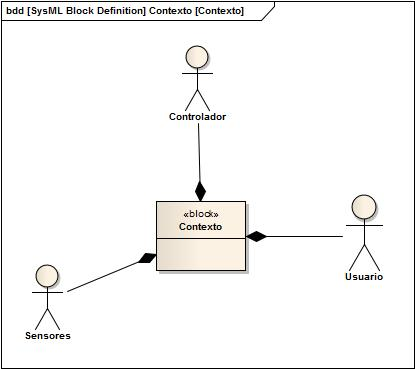
\includegraphics[width=0.80\textwidth, height = 9cm]{contexto1}
  \caption{Contexto del sistema}\label{fig:contexto1}
\end{figure}

% section caracteristicas_generales (end)

\section{Método de desarrollo} % (fold)
\label{sec:metodo_de_desarrollo}

El método de desarrollo utilizado es el desarrollo iterativo con entrega incremental. Este modelo se ilustra en la figura \ref{fig:MetodoDeDesarrollo}. En esta metodología de desarrollo el trabajo se divide en iteraciones en las cuales el producto va evolucionando. 
Un aspecto fundamental para guiar el desarrollo incremental es priorizar los requerimientos y los objetivos en función del valor que aportan al cliente. De esta manera se van añadiendo nuevos requerimientos o mejorando los que ya se completaron. Al finalizar cada iteración se obtiene un prototipo funcional.

\begin{figure}[h]
  \centering
  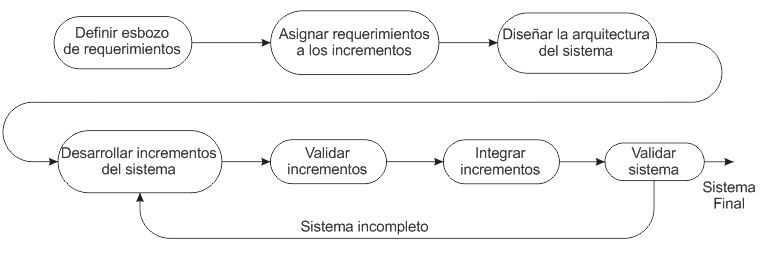
\includegraphics[width=0.80\textwidth, height = 4cm]{MetodoDeDesarrollo}
  \caption{Desarrollo incremental}\label{fig:MetodoDeDesarrollo}
\end{figure}

% section metodo_de_desarrollo (end)

\section{Casos de uso} % (fold)
\label{sec:casos_de_uso}

Dado el contexto, el sistema se puede describir de una manera general mediante un diagrama de caso de uso. El diagrama puede verse en la figura \ref{fig:casouso1}. En esta figura, se puede ver plasmados los requerimientos.

\begin{figure}[h]
  \centering
  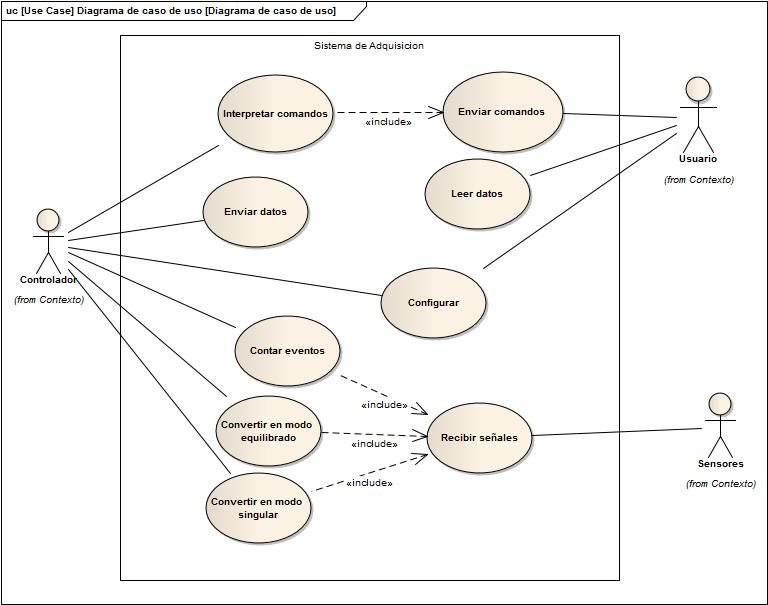
\includegraphics[width=0.80\textwidth, height = 11cm]{casouso1}
  \caption{Diagrama de caso de uso del sistema de adquisición}\label{fig:casouso1}
\end{figure}

El caso de uso ``configurar'' esta generalizado. Las acciones que incluye este caso son:
\begin{itemize}
	\item Configurar la interfaz serial
	\item Configurar canal en modo singular
	\item Configurar canal en modo equilibrado
	\item Configurar contador de eventos
	\item Configurar ganancia del del conversor
	\item Configurar intervalo de medicion para conversion analogica
\end{itemize}

% section casos_de_uso (end)

% chapter introduccion (end)

\chapter{Marco teórico} % (fold)
\label{cha:marco_teorico}



\section{Conversión Analógico-Digital y El conversor Delta-Sigma}
\label{sec:conversion_analogica_digital_y_el_conversor_delta_sigma}



\subsection{Conversion analogico digital} % (fold)
\label{sub:conversion_analogico_digital}
%CITADO

Para poder medir ciertos fenómenos naturales, se utilizan sensores físicos que miden las magnitudes de estos fenómenos y las traducen en tensiones voltaicas en la salida. Una lectura de dicha tensión nos da una idea de la magnitud física de lo que se esta midiendo. Si se obtiene, a partir de esta tensión, datos digitales que la representen, es posible construir un software que realice determinadas acciones en función de datos provenientes de los sensores. Un conversor analógico-digital es un dispositivo que toma como entrada una señal analógica voltaica, y la convierte en datos digitales.

La salida de los sensores, que permiten al equipo electrónico interaccionar con el entorno, es  normalmente  una  señal  analógica,  continua  en  el tiempo.  En  consecuencia,  esta información  debe  convertirse  a  binaria  (cada  dato  analógico  decimal  codificado  a  una palabra formada por unos y ceros) con el fin de adaptarla a los circuitos procesadores y de presentación. Un convertidor analógico-digital (CAD) es un circuito electrónico integrado cuya salida es la palabra digital resultado de convertir la señal analógica de entrada. \\

La conversión a digital se realiza en dos fases: cuantificación y codificación. Durante la primera se  muestrea la entrada y a  cada valor analógico obtenido se asigna un valor o estado, que depende del número de bits del CAD. El valor cuantificado se codifica en binario en una palabra digital, cuyo número de bits depende de las líneas de salida del CAD. Estos dos procesos determinan el diseño del circuito integrado. \\

En la práctica, el proceso de conversión está sujeto a numerosas limitaciones resultado de los procesos de fabricación. Las más relevantes son el tiempo de conversión y la finitud del número de estados de salida. La conversión involucra un tiempo y, en consecuencia, supone  una  incertidumbre  que  limita  la  velocidad  máxima  de  la  entrada.  Los  valores discretos  del  proceso  de  cuantificación  llevan  consigo  un  error  y  una  limitación  de resolución del circuito. La elección del CAD en un diseño electrónico dependerá de la adaptación de sus rasgos a  los requerimientos de la aplicación. \cite{adc}

% subsection conversion_analogico_digital (end)



\subsection{Conversores de canal único, de canal pseudo diferencial, y de canal totalmente diferencial}
\label{sub:conversores_de_canal_unico_de_canal_pseudo_balanceado_y_de_canal_totalmente_balanceado}
%CITADO

Un Conversor Analógico-Digital puede obtener la señal de voltaje de entrada mediante tres métodos distintos: Canal único, Canal pseudo diferencial, y canal totalmente diferencial. \\

En general, lo mas simple es elegir aquella estructura que sea compatible con el sensor que se utiliza. Pero a pesar de eso, existen ciertas características que reúne cada estructura que deben considerarse. Si existe un circuito de acondicionamiento de señal entre el sensor y el conversor, también puede afectar a la decisión sobre que tipo de estructura utilizar. Algunos conversores son configurables y permiten elegir entre canal único y pseudo diferencial, o canal único y totalmente diferencial.\cite{tipos_canales}

\subsubsection{Canal único}
\label{subs:canal_unico}

Las entradas de canal único son suficientes para la mayoría de las aplicaciones. En este tipo de estructuras, la señal de entrada esta referenciada a la masa común del conversor. Esta masa es compartida por todas las entradas que estén configuradas en este modo. La figura \ref{fig:canalunico} ilustra el muestreo de una señal para esta estructura.

A diferencia de las totalmente diferenciales, las entradas de canal único son mas sensibles al ruido y al desfasaje de continua. El desfasaje de continua (DC Offset) es un fenómeno que ocurre cuando el nivel de continua en la señal es distinto de 0. El ruido en el canal y el desfasaje de continua reducen la amplitud dinámica de la señal de entrada, lo cual provoca que la calidad de la conversión sea menor.\cite{dc_offset}

Este tipo de entradas suelen utilizarse en aquellos casos en que la fuente que produce la señal y el conversor A/D están cerca uno del otro (Por ejemplo, en la misma placa de cobre), y por lo tanto el desfasaje de continua y el ruido no son tan presentes como en casos donde estén mas separados. También se puede incluir un circuito que adapte la señal y reduzca estos efectos no deseados.\cite{tipos_canales}

\begin{figure}[h]
  \centering
  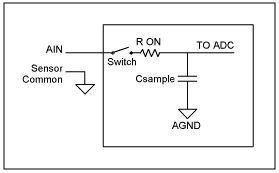
\includegraphics[width=0.60\textwidth, height = 4cm]{canalunico}
  \caption{Conversion de canal unico. La señal se toma midiendo la tension en el capacitor con respecto a una masa unica compartida por todos los canales del conversor}\label{fig:canalunico}
\end{figure}

% subsubsection canal_unico (end)

\subsubsection{Canal totalmente diferencial}
\label{subs:canal_totalmente_diferencial}

Una entrada totalmente diferencial es la que mayor inmunidad al ruido presenta. Como puede verse en la figura \ref{fig:totalmentediferencial}, cada una de las entradas esta conectada a un canal distinto del conversor. La medición final se calcula con la diferencia entre ambas entradas y no con respecto a masa, lo cual cancela el ruido entre ambas y elimina el desfasaje de continua. La desventaja de este conversor es que consume dos canales por cada señal en lugar de uno solo, como es en el caso de las estructuras de tipo canal único.\cite{tipos_canales}

\begin{figure}[h]
  \centering
  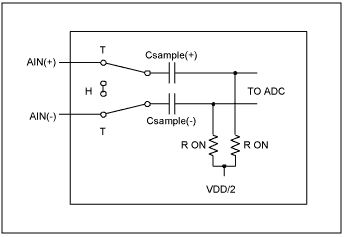
\includegraphics[width=0.80\textwidth, height = 6cm]{totalmentediferencial}
  \caption{Conversión totalmente diferencial. El valor que se mide esta dado por la diferencia entre ambas entradas, esto es lo que cancela el ruido presente en ambas señales, aumentando el rango dinámico de la conversión.}\label{fig:totalmentediferencial}
\end{figure}

% subsubsection canal_totalmente_diferencial (end)

\subsubsection{Canal pseudo-diferencial}
\label{subs:canal_pseudo_diferencial}

Las entradas pseudo-diferenciales son similares a las totalmente diferenciales en el hecho que separan la masa del conversor con la masa general, permitiendo que no haya desfasaje en continua en la señal. Pero no son una buena alternativa para eliminar ruido común.\cite{tipos_canales}


% subsubsection canal_pseudo_diferencial (end)

\subsection{Conversor Delta-Sigma} % (fold)
\label{sub:conversor_delta_sigma}

De manera básica, los conversores Delta-Sigma consisten en dos bloques: un bloque con un modulador Delta-Sigma, seguido de un bloque de filtro digital mas un decimador. El primer bloque aplica una técnica de muestreo de alta frecuencia a la señal analógica de entrada, produciendo a la salida una señal digital de 1 bit. El segundo bloque toma las muestras y las convierte en un código de menor frecuencia y mayor resolución. Existen dos frecuencias involucradas: La frecuencia de muestreo $f_s$ y la frecuencia de datos $f_d$. La figura \ref{fig:deltasigma} muestra el diagrama de bloques de este conversor.\cite{delta_sigma_1}

\begin{figure}[h]
  \centering
  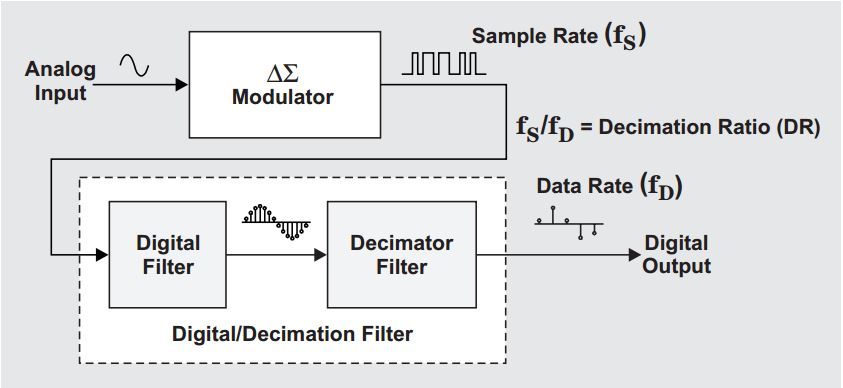
\includegraphics[width=0.80\textwidth, height = 6.3cm]{deltasigma}
  \caption{Diagrama de bloques del conversor analógico digital Delta-Sigma. El primer bloque corresponde al modulador Delta-Sigma, y el segundo al filtro digital con filtro de decimación}\label{fig:deltasigma}
\end{figure}

\subsubsection{El modulador Delta-Sigma} % (fold)
\label{ssub:el_modulador_delta_sigma}

El modulador Delta-Sigma es el responsable de digitalizar la señal de entrada y reducir el ruido en frecuencias bajas. La arquitectura del modulador implementa una técnica conocida como modelado de ruido, que empuja las frecuencias del ruido fuera de la banda de interés, reduciendo así el ruido en la señal convertida. Esto hace que los convertidores Delta-Sigma sean apropiados para casos donde se trabaja con señales de entrada de baja frecuencia y se requiere alta precisión en la medición. \\

El modulador convierte la señal de entrada en un tren de pulsos de un bit a la salida. La razón entre los unos y los ceros en este tren de pulsos es lo que representa al voltaje de entrada. Ademas, contiene un integrador que realiza el efecto de modelado de ruido, empujando el ruido a bandas de frecuencia mas altas. La figura \ref{fig:modeladoderuido} muestra como la combinación de la técnica de muestreo de un bit con el modelado de ruido empujan el dominio del ruido a frecuencias mayores.\cite{delta_sigma_1}

\begin{figure}[h]
  \centering
  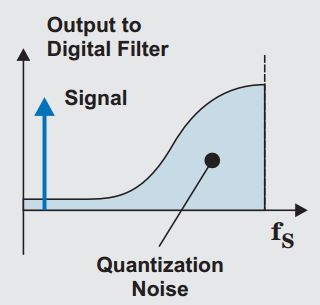
\includegraphics[width=0.40\textwidth, height = 4cm]{modeladoderuido}
  \caption{Ilustracion sobre como el modelado de ruido empuja las frecuencias de ruido a bandas que no perjudican a la medicion}\label{fig:modeladoderuido}
\end{figure}

% subsubsection el_modulador_delta_sigma (end)

\subsubsection{El filtro digital y filtro de decimacion} % (fold)
\label{ssub:el_filtro_digital_y_filtro_de_decimacion}

Una vez que la señal esta en el dominio digital, un filtro pasa-bajos digital se encarga de eliminar el ruido en alta frecuencia, y un filtro de decimacion se utiliza para disminuir la frecuencia de datos a la salida del conversor. \\

El filtro digital se implementa tomando las muestras del tren de pulsos de 1 bit y ponderando las muestras en un promedio. La frecuencia de salida del filtro digital es la misma que la frecuencia de muestreo. La figura \ref{fig:filtrodigital} muestra la salida del filtro en el dominio del tiempo y de la frecuencia. En el dominio del tiempo, puede verse que la salida de la señal se corresponde con la entrada analógica, que corresponde a una función seno. En el dominio de la frecuencia, puede verse como el ruido fue reducido por el filtro digital. La salida de este filtro es una onda muy parecida a la entrante, a una frecuencia alta. La cantidad de información es demasiada y no es necesaria. Por esto es que se aplica, luego del filtro digital, el filtro de decimacion. \\

\begin{figure}[h]
  \centering
  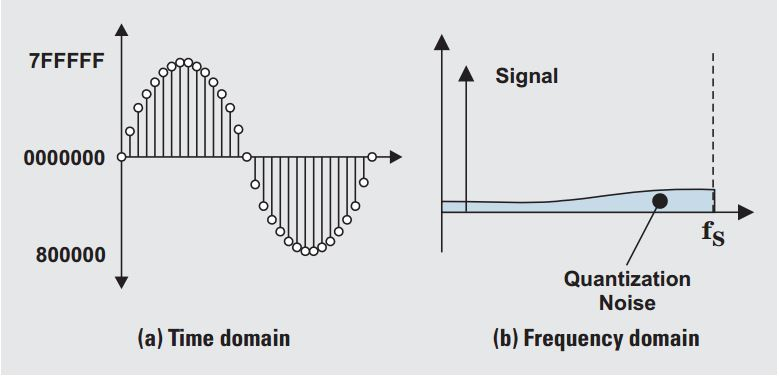
\includegraphics[width=0.80\textwidth, height = 6.3cm]{filtrodigital}
  \caption{Salida del filtro digital en el dominio del tiempo y de la frecuencia.}\label{fig:filtrodigital}
\end{figure}

El filtro de decimacion selecciona algunos datos de la señal de salida del filtro digital y descarta otros. La frecuencia de selección se denomina frecuencia de datos $f_s$ y es la frecuencia de salida del conversor. A pesar de que se elimina información, hay que recordar que no se elimina tanto como para no poder tener todos los datos necesarios acerca de la señal de entrada. Con el teorema de Nyquist\cite{shannon}, es posible reconstruir la señal de entrada sin perder información. La figura \ref{fig:decimacion} muestra el proceso de decimacion.\cite{delta_sigma_2} %http://lavryengineering.com/pdfs/lavry-sampling-theory.pdf

\begin{figure}[h]
  \centering
  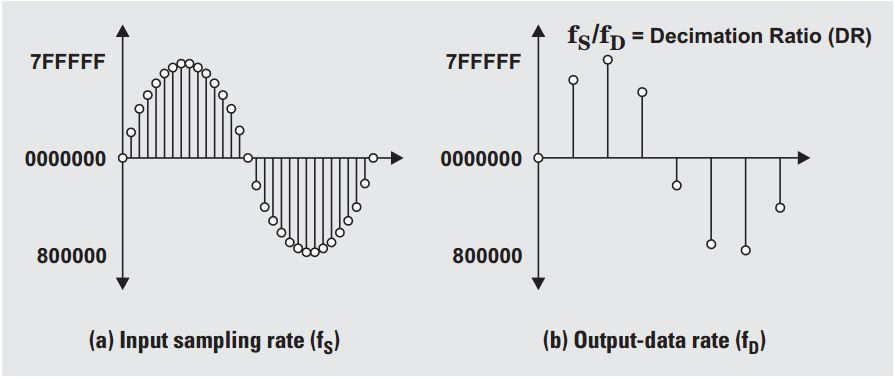
\includegraphics[width=0.80\textwidth, height = 6.3cm]{decimacion}
  \caption{Entrada (a) y salida (b) de la señal procesada por el filtro de decimacion. }\label{fig:decimacion}
\end{figure} 

% subsubsection el_filtro_digital_y_filtro_de_decimacion (end)


% subsection conversor_delta_sigma (end)

\section{Amplificadores de Instrumentación} %fold
\label{sec:amplificadores_de_instrumentacion}

%Bib: INSTRUMENTACIÓN ELECTRÓNICA DE COMUNICACIONES. José María Drake Moyano. UNIVERSIDAD DE CANTABRIA 2005.
%Bib: Apuntes de Clases, Electrónica 2. Universidad Nacional de Rosario Facultad de Ciencias Exactas, Ingeniería y Agrimensura Escuela de Ingeniería Electrónica.
%Bib: A Designer’s Guide to Instrumentation Amplifiers. 2da Edition, Charles Kitchin and Lew Count.

Los amplificadores de instrumentación surgen ante la necesidad de medir tensiones de muy bajo nivel, eliminando señales de interferencias e indeseadas (ruido) en modo común.
Se denomina amplificador de instrumentación a todo dispositivo creado a partir de amplificadores operacionales. Su diseño incluye:

\begin{itemize}
  \item Alta impedancia de entrada
    \item Alto rechazo de modo común
    \item Ganancia estable y variable con una única resistencia y que no se contraponga directamente la ganancia con el ancho de banda (fenómeno que suele suceder en los amplificadores operacionales).
\end{itemize}

Además está hecho con tensiones y corrientes de desequilibrio (offset) bajas y con pocas derivas e impedancia de salida baja.

En el circuito de la figura \ref{fig:aibasico} puede verse el esquema clásico para la realización de un amplificador de instrumentación, donde se ha colocado el circuito equivalente de la fuente de señal.

\begin{figure}[h]
  \centering
  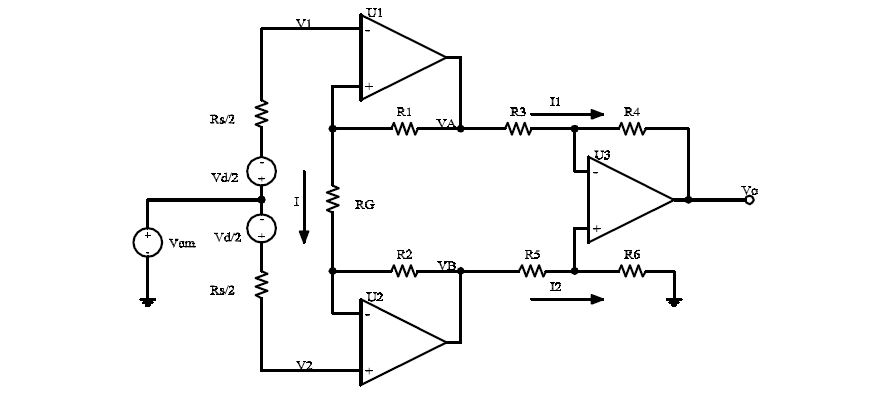
\includegraphics[width=0.60\textwidth, height = 4cm]{ai1}
  \caption{Amplificador Instrumental Básico}\label{fig:aibasico}
\end{figure}

El circuito está formado por una primera etapa con salida y entrada diferencial de alta impedancia, que amplifica únicamente la tensión diferencial de entrada; la segunda etapa es un amplificador diferencial con salida unipolar y ganancia en modo común nula idealmente.

Suponiendo amplificadores operacionales ideales: 

\begin{equation}\label{eq1}
I = \frac{V_1 - V_2}{R_g}  => \frac{R_1+R_2+R_g}{R_g} (V_d)
\end{equation}

Como la segunda etapa es un diferencial, si suponemos (R\textsubscript{3}R\textsubscript{6}=R\textsubscript{4}R\textsubscript{5}) y  (R\textsubscript{1}=R\textsubscript{2}) resulta la siguiente expresión de la tensión de salida:

\begin{equation}\label{eq2}
V_0 = \frac{R_6}{R_5}(1 +\frac{2R_1}{R_g} (V_d))
\end{equation}

En la segunda etapa:

\begin{equation}\label{eq3}
V_{cm}|_{2etapa} = \frac{V_A + V_B}{2}=V_{cm} +\frac{R_2 - R_1}{2R_g}(V_d)
\end{equation}

Podemos ver que la tensión en modo común vista por la segunda etapa es la misma que en la entrada mas un termino que depende de la tensión diferencial, producida por una variación del modo común en función de la tensión de entrada.

Entonces se llegan a las siguientes conclusiones:
\begin{enumerate}
\item La ganancia al modo común de la primera etapa es la unidad, siendo sus funciones:
\begin{itemize}
\item Amplificar la tensión diferencial.
\item Proporcionar un ajuste cómodo de la ganancia mediante R\textsubscript{g}.
\item Presentar una elevada impedancia de entrada.
\end{itemize}
\item El CMR (rechazo del modo común) depende del que presente la etapa diferencial de salida, y de la ganancia diferencial de la primera etapa.
\end{enumerate}

\subsection{Características de entrada de un Amplificador de Instrumentación} %fold
\label{sec:caract_entrada_amplificadores}
Evidentemente es deseable aproximarse al máximo a las características del amplificador de instrumentación ideal, se mostrará las características no ideales de estos dispositivos, considerando el modelo de amplificador de instrumentación real de la figura \ref{fig:aireal}.

\begin{figure}[h]
  \centering
  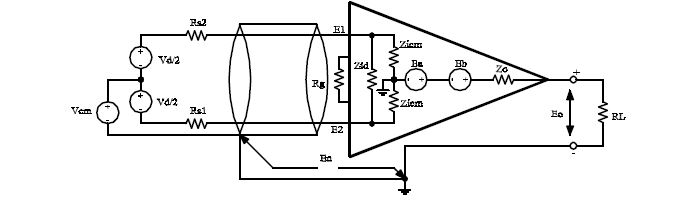
\includegraphics[width=1.0\textwidth, height = 4cm]{ai2}
  \caption{Modelo de un amplificador de instrumentación real.}\label{fig:aireal}
\end{figure}

\subsubsection{Impedancia de Entrada} %fold
\label{impedancia_entrada}
Si consideramos que las impedancias de entrada son infinitas, entonces debería existir un error en la ganancia efectiva debido a la resistencia de salida de la fuente.

La impedancia Z\textsubscript{id} representa la impedancia de entrada diferencial, que depende de R\textsubscript{g} y por eso también de la ganancia diferencial.

La impedancia de entrada en modo común Z\textsubscript{icm} está representada por dos componentes iguales entre cada entrada y masa. Esta impedancia puede haber sido medida de dos formas:

\begin{itemize}
\item Como la existente entre cada entrada por separado y masa, siendo entonces su representación en el circuito equivalente a la mostrada en la figura \ref{fig:aireal}.
\item Como la medida entre las dos entradas cortocircuitadas y masa. En este método obtendremos evidentemente la mitad que en la anterior.
\end{itemize}

La impedancia de entrada diferencial, debido a la resistencia de salida de la fuente de señal, nos va a producir una pérdida de ganancia. El error de ganancia supuesto R\textsubscript{s}=R\textsubscript{s1}+R\textsubscript{s2}, tendrá el valor:

\begin{equation}\label{eq4}
1 - \frac{Z_{id}}{Z_{id}+R_{s}}= \frac{R_{s}}{Z_{id}+R_{s}}
\end{equation}

Debemos tener en cuenta que el Z\textsubscript{icm} sea igual en las dos entradas, y que las resistencias de salidas de la fuente de señal también sean iguales, sino la señal se dividirá de manera desigual en las dos entradas produciendo una tensión diferencial, debido al modo común, no pudiendo separar la señal que si se quiere amplificar. Si se produce esta tensión diferencial se vería deteriorado sensiblemente el CMR del circuito.

%subsubsection impedancia_entrada (end)

\subsubsection{No Linealidad} %fold
\label{no_linealidad}

La linealidad de la función de transferencia de un amplificador se mide
respecto al caso ideal que correspondería con una función de transferencia constituida
por una recta, tal y como se representa en la figura \ref{fig:linealidad}.

\begin{figure}[h]
  \centering
  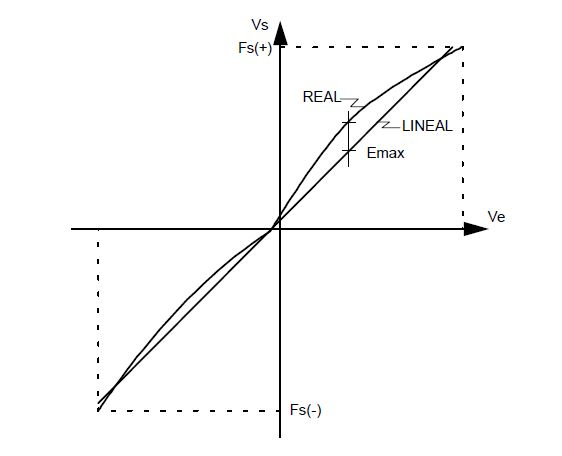
\includegraphics[width=0.60\textwidth, height = 4cm]{ai4}
  \caption{No linealidad de la función de transferencia de un amplificador de instrumentación.}\label{fig:linealidad}
\end{figure}

Existen varias definiciones de linealidad según la recta que consideremos. Nosotros vamos a usar la recta que mejor se adapte a la función de transferencia del amplificador, que suele ser la utilizada por los fabricantes cuando nos dan la linealidad de un AI integrado. Esta recta no tiene por qué pasar por el origen, ni presentar la pendiente marcada por la ganancia esperada del AI. Tiene que ser aquella que nos de el menor valor de no linealidad (NL), definida como:

\begin{equation}\label{eq5}
NL = \frac{|Salida Real - Salida lineal|_{max}}{Margen de variacion de la salida entre fondos de escala}
\end{equation}

%subsubsection no_linealidad (end)

\subsubsection{Rechazo al Modo Común} %fold
\label{rechazo_CMR}

Como se ve en la figura \ref{fig:aireal}, la tensión de salida tiene dos componentes. Uno de ellos es proporcional a la tensión de entrada diferencial y el otro a la tensión de modo común. La tensión de modo común que aparece entre los terminales de entrada del amplificador se define como: 

\begin{equation}\label{eq6}
E_{cm} = \frac{(E_{2}+E{1})}{2}
\end{equation}

Esta puede consistir en una cierta tensión de modo común de la fuente más cualquier tensión de ruido, E\textsubscript{n}, entre el común de la fuente y el del amplificador. La constante G\textsubscript{d} representa el factor de ganancia del amplificador diferencial (fijado por la resistencia exterior de selección de ganancia), mientras que la constante G\textsubscript{g}/CMR representa la ganancia al modo común del amplificador. El CMRR (relación de rechazo al modo común) está directamente relacionado con la ganancia diferencial y aumenta cuando lo hace esta. 

Idealmente deben seguir la misma progresión, es decir si G\textsubscript{d} aumenta 20 dB el CMRR debería aumentar 20dB (suponiendo que G\textsubscript{cm} se mantiene constante); pero en los circuitos reales esto no se cumple y el aumento de CMRR es menor. Se expresa habitualmente para los valores máximo y mínimo de la ganancia del amplificador y se mide en decibelios.

%subsection rechazo_CMR (end)

\subsubsection{Tensión de Offset} %fold
\label{tension_off}
La mayoría de los Amplificadores de Instrumentación son dispositivos de dos etapas: tienen una etapa de entrada de ganancia variable y otra de salida de ganancia fija. Por lo tanto podemos definir los siguientes parámetros:

\begin{itemize}
\item V\textsubscript{IOS} (Tensión de offset de la etapa de entrada): Es la tensión que debe aplicarse a la entrada de la etapa de entrada para forzar que su salida sea nula.
\item V\textsubscript{OOS} (Tensión offset de la etapa de salida) : Es la tensión que deberá aplicarse, en el caso de que sea accesible, a la entrada de la etapa de salida para producir una salida de cero voltios.
\item  V\textsubscript{OS} (Tensión offset global) : Es la tensión total de offset, referida a la entrada. Considerando que la etapa de entrada es la que presenta la ganancia diferencial del amplificador de instrumentación (a la segunda etapa se le suele asignar la unidad), la expresión del voltaje offset total será la siguiente:

\begin{equation}\label{eq7}
V_{OS} = V_{IOS} + \frac{V_{OOS}}{G_d}
\end{equation}

Podemos ver que a la salida tendremos un offset total de V\textsubscript{OOS} G\textsubscript{d}.
\end{itemize}

%subsubsection tension_off (end)

%subsection caract_entrada_amplificadores (end)

\subsection{Amplificadores de Instrumentación con Ganancia Programable} %fold
\label{ganancia_programable}

Se pueden incorporan en los montajes de los amplificadores de instrumentación una red de resistencias seleccionables digitalmente, para hacer las veces de R\textsubscript{G} y así poder cambiar el valor de la ganancia mediante un control digital, desde por ejemplo el sistema de adquisición de datos, constituyendo lo que se denomina amplificador de instrumentación de ganancia programable. Un amplificador de este tipo se puede realizar mediante componentes
discretos, utilizando resistencias y puertas analógicas, pero las características obtenidas serán, en la mayoría de las ocasiones, sensiblemente inferiores a las de los dispositivos integrados.

En la figura \ref{fig:programable}  se puede ver el esquema del amplificador de instrumentación con ganancia programable PGA206/207 de Burr-Brown. La ganancia de este amplificador se puede controlar por medio de las entradas A1 y A2 para conseguir ganancias de 1, 2, 4 u 8.

\begin{figure}[h]
  \centering
  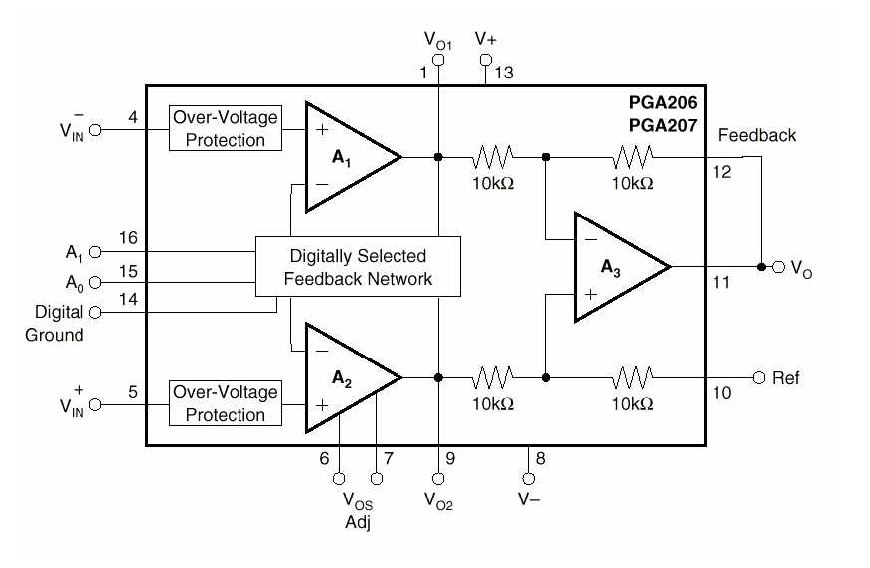
\includegraphics[width=1.0\textwidth, height = 7cm]{ai5}
  \caption{Amplificador de Instrumentación programable PGA206.}\label{fig:programable}
\end{figure}

En este modelo las entradas analógicas están protegidas contra sobretensiones de hasta 40 voltios, incluso sin alimentación. Las resistencias internas están ajustadas por láser para conseguir una baja tensión de offset y pequeñas derivas.

La entrada puede provenir de un sistema multicanal multiplexado puesto que el amplificador tiene un tiempo de asentamiento muy corto. Además las entradas tipo FET eliminan los errores debidos a la corriente de polarización y a la resistencia parásita serie asociada a los multiplexores analógicos.


% subsection ganancia_programable (end)

%section amplificadores_de_instrumentacion (end)

\section{Sistema de control para motor sin escobillas} % (fold)
\label{sec:sistema_de_control_para_motor_sin_escobillas}

%Bib : Control motor brushless sensorless. Trabajo de Fin de Grado. Gonzalo Solchaga y Jesus Maria Corres Sanz. Junio 2015.
%Bib : Desarrollo de un controlador para motores DC brushless basado en CompactRIO y LabVIEW de National Instruments para el estudio de nuevos algoritmos de control.Proyecto fin de carrera. Juan Miguel Garcia Haro. 2011
%Bib: http://www.digikey.com/en/articles/techzone/2013/mar/an-introduction-to-brushless-dc-motor-control

\subsection{Motor DC sin escobillas (Motores Brushless)}
\label{subsec: motor_sin_escobillas}

Los motores DC brushless no emplean escobillas en la conmutación para la transferencia de energía, estas producen rozamiento, disminuyen el rendimiento, generan calor, son ruidosos y demandan una sustitución periódica y, por tanto, un mayor mantenimiento.

Algunas de las ventajas de los motores BLDC con respecto a los motores DC convencionales son:

\begin{itemize}
\item Mejor relación velocidad-par motor.
\item Mayor respuesta dinámica.
\item Mayor eficiencia.
\item Menor ruido
\item Mayor vida útil.
\item Mayor rango de velocidad.
\item Mejor relación par motor - tamaño (por lo que son mejores en para los espacios reducidos).
\end{itemize}

%subsection sistemas_sin_escobillas (end)

\subsection{Clasificación de Motores sin Escobillas}
\label{clasificacion_motores}

Los motores DC Brushless se clasifican en dos: 

\begin{enumerate}
\item Inrunner.
\item Outrunner.
\end{enumerate}

Los Inrunner desarrollan mayor velocidad y suelen ser mas pequeños, entregan su máximo torque a muy altas revoluciones por minuto (RPM), por lo que se usan siempre con engranajes reductores. En estos motores el elemento móvil es el eje, sobre el cual se encuentran instalados los imanes permanentes.

Los motores Outrunner desarrollan su torque máximo a velocidades mas bajas, por lo que usualmente no necesitan reducción, y se pueden acoplar directamente a una hélice. En estos los imanes permanentes están instalados en la carcasa externa del motor, que en este caso es la que gira y el bobinado se encuentra fijado al eje.

Estos motores trabajan por medio de variadores, también llamados controladores de velocidad (electronic speed controler o ESC), que transforman la corriente continua de las baterías en una tensión alterna trifásica y la alimentan a los bobinados en cierta secuencia dependiendo de la posición del rotor.
Para manejar los motores se precisa el conocimiento de la posición del rotor en cada momento, para lo cual se utilizan dos técnicas básicamente, dependiendo de la existencia o no de sensores en el motor, lo que los divide en dos familias: con sensores (sensored) y sin sensores (sensorless).

\begin{itemize}
  \item Con sensores: Disponen de sensores de efecto hall o de encoders que indican la posición del rotor. Es habitual que tengan 3 sensores separados 120\textsuperscript{o}, uno para cada bobinado del motor.
  \item Sin sensores: No tienen sensores; la posición se determina mediante la medición del efecto de la fuerza contraelectromotriz sobre las bobinas
\end{itemize}





%subsection clasificacion_motores (end)

\subsection{Métodos de Control de Motores sin Escobillas}
\label{subsection: metodos_control_motores}

Los sistemas utilizados para el control con sensores se clasifican según el algoritmo utilizado. Los mas utilizados son los siguientes: 

\begin{itemize}
\item Conmutación trapezoidal o "six step mode".
\item Conmutación sinusoidal.
\item Control vectorial o Field Oriented Control.
\end{itemize}

\subsubsection{Conmutación trapezoidal}
\label{conmutacion_trapezoidal}

Es el método más simple de control de los motores sin escobillas. En este esquema se controla la corriente que circula por los terminales del motor, excitando un par simultáneamente y manteniendo el tercer terminal desconectado. Sucesivamente se va alternando el par de terminales a excitar hasta completar las seis combinaciones posibles. Las seis direcciones de las corrientes se muestran en la figura \ref{fig:trapezoidal}

\begin{figure}[h]
  \centering
  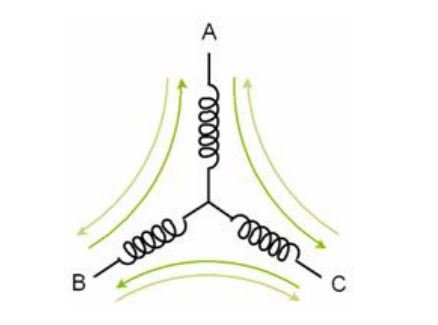
\includegraphics[width=1.0\textwidth, height = 7cm]{m1}
  \caption{Esquema de las seis posibles direcciones de circulación de corriente.}\label{fig:trapezoidal}
\end{figure}

Tiene como ventajas su sencillez y facilidad de implementación por lo cual es el método más usado en motores pequeños. Pese a esto, tiene un problema inherente a la conmutación del vector de corrientes que es un rizado en el torque de salida. En aplicaciones donde se requieren fuerzas uniformes o bajas velocidades, esto puede llegar a ser inconveniente. En la figura \ref{fig:corrientes_bobinas} se muestran las corrientes por cada una de las fases, la secuencia de conmutación y el torque.

\begin{figure}[h]
  \centering
  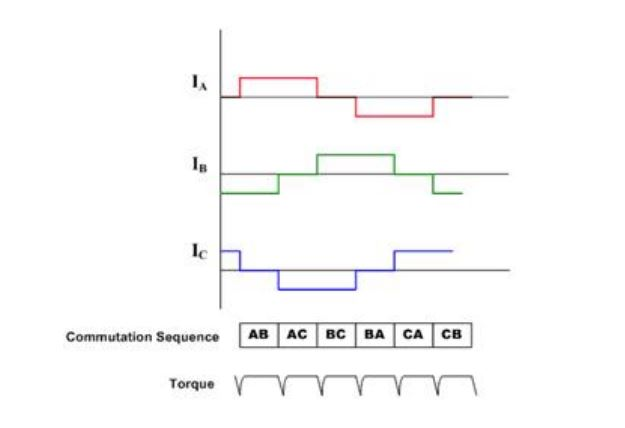
\includegraphics[width=1.0\textwidth, height = 7cm]{m2}
  \caption{: Corrientes en las bobinas y torque del motor.}\label{fig:corrientes_bobinas}
\end{figure}

\cite{brushless_control}

%subsubsection conmutacion_trapezoidal (end)

\subsubsection{Conmutación Sinusoidal}
\label{subsubsection: conmutacion_sin}

Es un método de control mas eficiente que el la conmutación trapezoidal, ya que intenta controlar la posición del rotor en continuamente.

Esta continuidad se consigue aplicando simultáneamente tres corrientes sinusoidales
desfasadas 120\textsuperscript{o} a los tres bobinados del motor. La fase de estas corrientes se escoge de forma que el vector de corrientes resultante siempre esté en cuadratura con la orientación del rotor y tenga un valor constante.

Como consecuencia de este procedimiento se obtiene un par más preciso y sin el rizado típico de la conmutación trapezoidal. No obstante, para poder generar dicha modulación sinusoidal es necesaria una medida precisa de la posición del rotor, que difícilmente se logra con sensores de efecto Hall, por lo cual se requiere de un encoder absoluto de alta resolución.

A bajas velocidades este método de control presenta el mejor desempeño en eficiencia y suavidad del torque, sin embargo a altas frecuencias no responde tan bien debido a la necesidad de procesar señales sinusoidales de frecuencias altas y a que los controladores PI usados para generar estas señales tienen una respuesta limitada en ganancia y frecuencia. Cuando la frecuencia es suficientemente alta, la eficiencia decrece y el error aumenta, tendiendo a un punto de cero torque.
%subsubsection conmutacion_sin (end)

\subsubsection{Control Vectorial}
\label{subsubsection: control_vectorial}

El problema principal que presenta la conmutación sinusoidal es que intenta controlar directamente las corrientes que circulan por el motor, las cuales son intrínsecamente variantes en el tiempo. Al aumentar la velocidad del motor, y por tanto la frecuencia de las corrientes, empiezan a aparecer problemas.

\begin{figure}[h]
  \centering
  \includegraphics[width=1.0\textwidth, height = 7cm]{control_vectorial}
  \caption{: Diagrama de Bloques del Control Vectorial.}\label{fig:control_vectorial}
\end{figure}

El control vectorial o Field Oriented Control (FOC) soluciona el problema controlando el vector de corrientes directamente en un espacio de referencia ortogonal y rotacional, llamado espacio D-Q (Direct - Quadrature) como se muestra en la figura . Dicho
espacio de referencia está normalmente alineado con en el rotor de forma que permite que el control del flujo y del par del motor se realice de forma independiente. La componente directa permite controlar el flujo y la componente en cuadratura el par. Para este fin se requiere no solamente una muy buena medición de la orientación del rotor, sino un tratamiento matemático previo de las señales para transformarlas del marco trifásico estático de los bobinados en el estator (circuito fijo dentro del cual gira el rotor) al marco rotacional D-Q del rotor. Este es el control que presenta mejor respuesta en todos los rangos de velocidad pero resulta ser el más costoso de implementar, lo cual lo hace inadecuado para toda aplicación en la que no sea estrictamente necesario.

%subsubsection control_vectorial (end)

%subsection metodos_control_motores (end)


\pagebreak

\subsubsection{Banco de Ensayos para Motores}
\label{subsubsection: banco_ensayos}

%Bib: Proyecto de Fin de Carrera."Sistemas de adquisición de datos y control en tiempo real para bancos de ensayos de motores". Rodriguez Luis Gustavo y Maffei Ignacio.

El siguiente extracto está basado en la tesis de Rodriguez Luis Gustavo y Maffei Ignacio, "Sistemas de adquisición de datos y control en tiempo real para bancos de ensayos de motores", realizada en el Laboratorio de Arquitectura de Computadoras (LAC), Facultad de Ciencias Exactas Físicas y Naturales, UNC.

Para realizar ensayos a un motor es necesario instalarlo en un banco de pruebas o de ensayos. Este consta básicamente de los siguientes elementos:

\begin{itemize}
\item Cimentación: absorbe las vibraciones que se producen debido a la existencia en el motor de fuerzas de inercia no equilibradas y de los correspondientes momentos resultantes.
\item Bancada: soporta el motor ensayado.
\item Soporte: permite montar y fijar el motor en la bancada, así como regular la altura y alinear el motor con el freno.
\item Freno dinamométrico: absorbe la potencia desarrollada por el motor, ofreciendo una resistencia al giro de éste, y debe estar provisto de dispositivo para medir el par motor.
\item Eje de Transmisión: Permite la unión mecánica del freno con el motor, con una cierta elasticidad y capacidad de absorber desalineaciones.
\item Amortiguador torsional: su función es de amortiguar el movimiento alternativo del motor y las vibraciones del motor para que no influyan en el dinamómetro.
\item Sistema de combustible: se debe suministrar el combustible al motor mediante cañerías directo desde un tanque de combustible o a través de los instrumentos de medición de consumo.
\item Sistema de refrigeración del motor: si los motores son refrigerados por agua, normalmente se utiliza la bomba de agua del propio motor. Esta impulsa el agua a través del motor hacia un intercambiador de calor (agua/agua o agua/aire), en general con regulación termostática por medio de válvulas.
Si los motores son refrigerados por aire se suele utilizar un ventilador dirigido hacia las aletas del motor.
\item Sistema de refrigeración de aceite: en ocasiones también se refrigera el aceite del motor, ya que al no existir una corriente de aire al cárter, éste tiende a sobrecalentarse. El sistema consta de un intercambiador aceite/agua y en ocasiones una bomba auxiliar.
\item Sistema de refrigeración del dinamómetro: los frenos dinamométricos por corrientes de Foucault y los hidráulicos transforman toda la energía mecánica que reciben del motor en calor. Este calor es eliminado por el sistema de refrigeración del freno, que suele ser mediante el abastecimiento continuo de agua a través de un circuito cerrado.
\item Red de agua: es un circuito cerrado cuya función es disminuir la temperatura del agua proveniente del dinamómetro y del intercambiador de calor del agua y aceite del motor.
\item Sistema de ventilación de la sala: se debe evitar el sobrecalentamiento de la sala por la radiación de calor del motor. Se efectúa mediante ventiladores axiales o centrífugos de impulsión y extracción.
\item Sistema de evacuación de los gases de escape del motor: los gases de escape deben ser enviados a la atmósfera, tras pasar por una cámara de expansión.
\item Sistema de arranque: este sistema permite poner en marcha el motor a ensayar sin necesidad de contar con el motor de arranque original del motor.
\item Elementos de medición: los elementos principales de medición son:

\begin{itemize}
\item Taquímetro: mide la velocidad angular del motor (rpm).
\item Celda de carga: mide el torque ejercido por el motor.
\item Sensor temperatura de motor y del dinamómetro.
\item Sensor presión de aceite del motor y del dinamómetro.
\item Sensor de temperatura, presión, y humedad ambiente.
\item Caudalímetro de aire y combustible.
\item Sensores de otras temperaturas y presiones.
\item etc.
\end{itemize}

\end{itemize}

%subsection banco_ensayos (end)

% section sistema_de_control_para_motor_sin_escobillas (end)

\section{Sistemas de comunicación serie con inmunidad al ruido} % (fold)
\label{sec:sistemas_de_comunicacion_serie_con_inmunidad_al_ruido}

%CITADO

\subsection{Comunicacion serial} % (fold)
\label{sub:comunicacion_serial}
%que es la comunicacion serial? http://digital.ni.com/public.nsf/allkb/039001258CEF8FB686256E0F005888D1

La comunicación serial es un protocolo de comunicación de transmisión asincrónica entre dispositivos, que se incluye de manera estándar en prácticamente cualquier computadora. La mayoría de las computadoras incluyen dos puertos seriales RS-232. La comunicación serial es también un protocolo común utilizado por varios dispositivos para instrumentación; existen varios dispositivos compatibles con GPIB que incluyen un puerto RS-232. Además, la comunicación serial puede ser utilizada para adquisición de datos si se usa en conjunto con un dispositivo remoto de muestreo.

El concepto de comunicación serial es sencillo. El puerto serial envía y recibe bytes de información un bit a la vez. Aun y cuando esto es más lento que la comunicación en paralelo, que permite la transmisión de un byte completo por vez, este método de comunicación es más sencillo y puede alcanzar mayores distancias. Por ejemplo, la especificación IEEE 488 para la comunicación en paralelo determina que el largo del cable para el equipo no puede ser mayor a 20 metros, con no más de 2 metros entre cualesquier dos dispositivos; por el otro lado, utilizando comunicación serial el largo del cable puede llegar a los 1200 metros.

Típicamente, la comunicación serial se utiliza para transmitir datos en formato ASCII. Para realizar la comunicación se utilizan 3 líneas de transmisión: Tierra (o referencia), Transmitir, Recibir. Debido a que la transmisión es asincrónica, es posible enviar datos por un línea mientras se reciben datos por otra. Existen otras líneas disponibles para realizar handshaking, o intercambio de pulsos de sincronización, pero no son requeridas. Las características más importantes de la comunicación serial son la velocidad de transmisión, los bits de datos, los bits de parada, y la paridad. Para que dos puertos se puedan comunicar, es necesario que las características sean iguales.\cite{intro_serial}

\subsubsection{Conceptos} % (fold)
\label{ssub:conceptos}

\begin{itemize}
  \item \textbf{Velocidad de transmisión (baud rate):} Indica el número de bits por segundo que se transfieren, y se mide en baudios. Por ejemplo, 300 baudios representa 300 bits por segundo. Cuando se hace referencia a los ciclos de reloj se está hablando de la velocidad de transmisión. Por ejemplo, si el protocolo hace una llamada a 4800 ciclos de reloj, entonces el reloj está corriendo a 4800 Hz, lo que significa que el puerto serial está muestreando las líneas de transmisión a 4800 Hz. Las velocidades de transmisión más comunes para las lineas telefónicas son de 14400, 28800, y 33600. Es posible tener velocidades más altas, pero se reduciría la distancia máxima posible entre los dispositivos. Las altas velocidades se utilizan cuando los dispositivos se encuentran uno junto al otro, como es el caso de dispositivos GPIB.
  \item \textbf{Bits de datos:} Se refiere a la cantidad de bits en la transmisión. Cuando la computadora envía un paquete de información, el tamaño de ese paquete no necesariamente será de 8 bits. Las cantidades más comunes de bits por paquete son 5, 7 y 8 bits. El número de bits que se envía depende en el tipo de información que se transfiere. Por ejemplo, el ASCII estándar tiene un rango de 0 a 127, es decir, utiliza 7 bits; para ASCII extendido es de 0 a 255, lo que utiliza 8 bits. Si el tipo de datos que se está transfiriendo es texto simple (ASCII estándar), entonces es suficiente con utilizar 7 bits por paquete para la comunicación. Un paquete se refiere a una transferencia de byte, incluyendo los bits de inicio/parada, bits de datos, y paridad. Debido a que el número actual de bits depende en el protocolo que se seleccione, el término paquete se usar para referirse a todos los casos.
  \item \textbf{Bits de parada:} Usado para indicar el fin de la comunicación de un solo paquete. Los valores típicos son 1, 1.5 o 2 bits. Debido a la manera como se transfiere la información a través de las líneas de comunicación y que cada dispositivo tiene su propio reloj, es posible que los dos dispositivos no estén sincronizados. Por lo tanto, los bits de parada no sólo indican el fin de la transmisión sino además dan un margen de tolerancia para esa diferencia de los relojes. Mientras más bits de parada se usen, mayor será la tolerancia a la sincronía de los relojes, sin embargo la transmisión será más lenta.
  \item \textbf{Paridad:} Es una forma sencilla de verificar si hay errores en la transmisión serial. Existen cuatro tipos de paridad: par, impar, marcada y espaciada. La opción de no usar paridad alguna también está disponible. Para paridad par e impar, el puerto serial fijará el bit de paridad (el último bit después de los bits de datos) a un valor para asegurarse que la transmisión tenga un número par o impar de bits en estado alto lógico. Por ejemplo, si la información a transmitir es 011 y la paridad es par, el bit de paridad sería 0 para mantener el número de bits en estado alto lógico como par. Si la paridad seleccionada fuera impar, entonces el bit de paridad sería 1, para tener 3 bits en estado alto lógico. La paridad marcada y espaciada en realidad no verifican el estado de los bits de datos; simplemente fija el bit de paridad en estado lógico alto para la marcada, y en estado lógico bajo para la espaciada. Esto permite al dispositivo receptor conocer de antemano el estado de un bit, lo que serviría para determinar si hay ruido que esté afectando de manera negativa la transmisión de los datos, o si los relojes de los dispositivos no están sincronizados.
\end{itemize}\cite{intro_serial}

% subsubsection conceptos (end)

% subsection comunicacion_serial (end)

\subsection{Implementando la inmunidad al ruido en comunicaciones seriales} % (fold)
\label{sub:implementando_la_inmunidad_al_ruido_en_comunicaciones_seriales}

En un sistema complejo, puede existir ruido proveniente de varias fuentes distintas. Esto incluye al ruido del ambiente, como el de la fuente de alimentación, etcétera. Las fuentes que producen ruido presentan una amenaza a fallos de datos en una comunicación serial. En esta sección se mencionan diversas técnicas aplicables a la tecnología de comunicación serial, que disminuyen el ruido presente, disminuyendo la tasa de errores.\cite{ruido_serial}

\begin{itemize}
  \item \textbf{Filtro RC externo:} Un filtro RC pasa-bajos externo es una manera de inmunizar el sistema al ruido en altas frecuencias, pero presenta el problema de empeorar la velocidad de los flancos de subida en el canal de comunicación y agrega una carga a los pines involucrados. Un flanco lento es mas susceptible al ruido y puede causar inestabilidad en el sistema. Para resultados óptimos, es necesario realizar un balance entre la reducción de ruido y la reducción en la velocidad del flanco. El balance se obtiene cambiando los valores de las resistencias involucradas en el filtro. Los valores dependerán del valor de reducción de ruido requerido y la tensión de alimentación
  \item \textbf{Fuente de alimentación desacoplada:} Hay ocasiones en las que el ruido proveniente de la fuente de alimentación puede causar errores en la comunicación. La reducción de este ruido se puede alcanzar utilizando filtros LC, también llamados ``Ferrite Beads''. Estos dispositivos son inductores hechos específicamente para ser colocados en serie con el cable de alimentación para reducir el ruido en alta frecuencia producido por la fuente. Típicamente, se suelen colocar capacitores de distintos valores luego del inductor para mejorar el filtrado. 
  \item \textbf{Filtros digitales:} También es posible utilizar filtros digitales para reducir ruido. Esto se suele ver sobretodo en diseño de sistemas FPGA. Los filtros digitales pueden ser realizados en VHDL o Verilog, y filtran tanto la señal de datos como la señal del clock. Los distintos parámetros del filtro están dados en la frecuencia de oscilación y el tiempo de filtrado deseado. 
\end{itemize}

% subsection implementando_la_inmunidad_al_ruido_en_comunicaciones_seriales (end)

% section sistemas_de_comunicacion_serie_con_inmunidad_al_ruido (end)

\section{Medición de frecuencia de RPM} % (fold)
\label{sec:medicion_de_frecuencia_de_rpm}
%CITADO

Un tacometro es un dispositivo digital que mide e indica la velocidad de un objeto en rotación. Un objeto en rotación puede ser un ventilador, la rueda de un auto, o cualquier cosa que esta en movimiento de revolución. Los tacometros digitales se pueden clasificar en cuatro tipos dependiendo de la técnica de adquisición de datos y la técnica de medición.

Basándose en la técnica de adquisición de datos, los tacometros digitales pueden ser de tipo:

\begin{itemize}
  \item \textbf{Con contacto:} El dispositivo de medición esta en contacto con la pieza de revolución que se utiliza para medir. 
  \item \textbf{Sin contacto:} El dispositivo de medición no esta conectado físicamente al motor. Se suele utilizar un láser para determinar la velocidad de la pieza de revolución
\end{itemize}

Basándose en la técnica de medición, pueden ser:

\begin{itemize}
  \item \textbf{Medición de tiempo:} Calcula la velocidad calculando el tiempo entre los pulsos medidos. Suelen ser mas precisos en velocidades bajas.
  \item \textbf{Medición de frecuencia:} Calcula la velocidad midiendo la frecuencia de los pulsos en un intervalo de tiempo. Suelen ser mas precisos en velocidades altas.
\end{itemize}

\subsection{Medición con fotointerruptor o sensor óptico} % (fold)
\label{sub:medicion_con_fotointerruptor_o_sensor_optico}
%http://www.utopiamechanicus.com/article/arduino-photo-interruptor-slotted-optical-switch/

Un fotointerruptor es un dispositivo que contiene dos extremos de los cuales de uno se emite luz y del otro se recibe mediante un fotosensor. En la figura \ref{fig:fotointerruptor} se puede ver un ejemplo de uno de ellos. Con este dispositivo, es posible implementar un tacometro de adquisición sin contacto y medición de frecuencia.\cite{slotted_sensor}

\begin{figure}[h]
  \centering
  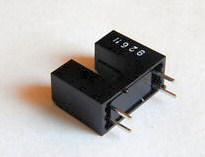
\includegraphics[width=0.20\textwidth, height = 3cm]{fotointerruptor}
  \caption{Fotointerruptor o sensor óptico}\label{fig:fotointerruptor}
\end{figure}

En el momento que el fotointerruptor esta conectado, se emite una luz infrarroja que va desde el lado emisor al receptor. Si se recibe luz, se genera una tensión (cuyo valor depende del fotointerruptor utilizado) en la salida del fotointerruptor, si no se recibe luz, se tienen 0 Volts a la salida. Un circuito típico puede verse en la figura \ref{fig:circuitotipico_fotointerruptor} \\

\begin{figure}[h]
  \centering
  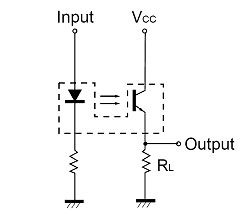
\includegraphics[width=0.30\textwidth, height = 5cm]{circuitotipico_fotointerruptor}
  \caption{Uso típico de un fotointerruptor}\label{fig:circuitotipico_fotointerruptor}
\end{figure}

Considerando el comportamiento de este dispositivo, es posible generar un generador de pulsos colocando algún objeto que obstruya el camino de la luz del fotointerruptor, y que esta obstrucción se de en cada vuelta del motor. Un ejemplo seria poner un aspa que gire con el eje, y que sea esta misma aspa la que obstruye la luz que va de un extremo a otro del fotointerruptor.

Esta señal de pulsos que sale del fotointerruptor puede servir como entrada a un microcontrolador que cuente los pulsos en un intervalo de tiempo, y así determinar la velocidad del motor.

% subsection medicion_con_fotointerruptor_o_sensor_optico (end)

% section medicion_de_frecuencia_de_rpm (end)

\section{Sistemas de base de datos para sistemas embebidos} % (fold)
\label{sec:sistemas_de_base_de_datos_para_sistemas_embebidos}

Una base de datos es un conjunto de datos pertenecientes a un mismo contexto y almacenados sistemáticamente para su posterior uso. En este sentido; una biblioteca puede considerarse una base de datos compuesta en su mayoría por documentos y textos impresos en papel e indexados para su consulta. Actualmente la mayoría de las bases de datos están en formato digital, siendo este un componente electrónico, y por ende se ha desarrollado y se ofrece un amplio rango de soluciones al problema del almacenamiento de datos.
Existen programas denominados sistemas gestores de bases de datos, abreviado DBMS, que permiten almacenar y posteriormente acceder a los datos de forma rápida y estructurada. Las propiedades de estos DBMS, así como su utilización y administración, se estudian dentro del ámbito de la informática.
MySQL es un sistema de gestion de base de datos muy conocido y muy usado actualmente. Existe una version de MySQL para sistemas embebidos, denominada SQLite. 

\subsection{MySQL} % (fold)
\label{sub:mysql}

MySQL es un sistema de gestión de bases de datos relacional, multihilo y multiusuario. Está escrito en C y C++ y emplea el lenguaje SQL para consultas a la base de datos.
MySQL es muy utilizado en aplicaciones web, como Drupal o phpBB, en plataformas (Linux/Windows-Apache-MySQL-PHP/Perl/Python), y por herramientas de seguimiento de errores como Bugzilla. Su popularidad como aplicación web está muy ligada a PHP, que a menudo aparece en combinación con MySQL.
MySQL es una base de datos muy rápida en la lectura cuando utiliza el motor no transaccional MyISAM, pero puede provocar problemas de integridad en entornos de alta concurrencia en la modificación. En aplicaciones web hay baja concurrencia en la modificación de datos y en cambio el entorno es intensivo en lectura de datos, lo que hace a MySQL ideal para este tipo de aplicaciones. Sea cual sea el entorno en el que va a utilizar MySQL, es importante monitorizar de antemano el rendimiento para detectar y corregir errores tanto de SQL como de programación.


% subsection mysql (end)

\subsection{SQLite} % (fold)
\label{sub:sqlite}


SQLite es un sistema de gestión de bases de datos relacional compatible con ACID, contenida en una relativamente pequeña (~275 kiB) biblioteca escrita en C. 
A diferencia de los sistemas de gestión de bases de datos cliente-servidor, el motor de SQLite no es un proceso independiente con el que el programa principal se comunica. En lugar de eso, la biblioteca SQLite se enlaza con el programa pasando a ser parte integral del mismo. El programa utiliza la funcionalidad de SQLite a través de llamadas simples a subrutinas y funciones. Esto reduce la latencia en el acceso a la base de datos, debido a que las llamadas a funciones son más eficientes que la comunicación entre procesos. El conjunto de la base de datos (definiciones, tablas, índices, y los propios datos), son guardados como un sólo fichero estándar en la máquina host. Este diseño simple se logra bloqueando todo el fichero de base de datos al principio de cada transacción.
En su versión 3, SQLite permite bases de datos de hasta 2 Terabytes de tamaño, y también permite la inclusión de campos tipo BLOB. (10) \cite{sqlite}

\subsubsection{Características} % (fold)
\label{ssub:caracteristicas}

La biblioteca implementa la mayor parte del estándar SQL-92, incluyendo transacciones de base de datos atómicas, consistencia de base de datos, aislamiento, y durabilidad (ACID), triggers y la mayor parte de las consultas complejas.
SQLite usa un sistema de tipos inusual. En lugar de asignar un tipo a una columna como en la mayor parte de los sistemas de bases de datos SQL, los tipos se asignan a los valores individuales. Por ejemplo, se puede insertar un string en una columna de tipo entero (a pesar de que SQLite tratará en primera instancia de convertir la cadena en un entero). Algunos usuarios consideran esto como una innovación que hace que la base de datos sea mucho más útil, sobre todo al ser utilizada desde un lenguaje de scripting de tipos dinámicos. Otros usuarios lo ven como un gran inconveniente, ya que la técnica no es portable a otras bases de datos SQL. SQLite no trataba de transformar los datos al tipo de la columna hasta la versión 3.
Varios procesos o hilos pueden acceder a la misma base de datos sin problemas. Varios accesos de lectura pueden ser servidos en paralelo. Un acceso de escritura sólo puede ser servido si no se está sirviendo ningún otro acceso concurrentemente. En caso contrario, el acceso de escritura falla devolviendo un código de error (o puede automáticamente reintentarse hasta que expira un tiempo de expiración configurable). Esta situación de acceso concurrente podría cambiar cuando se está trabajando con tablas temporales. Sin embargo, podría producirse un interbloqueo debido al multihilo. (11)

% subsubsection caracteristicas (end)
% subsection sqlite (end)

% section sistemas_de_base_de_datos_para_sistemas_embebidos (end)



% chapter marco_teorico (end)

\chapter{Iteracion 0: Orden de las iteraciones} % (fold)
\label{cha:iteracion_0}

\section{Introduccion} % (fold)
\label{it0:sec:introduccion}

El desarrollo de las iteraciones sigue un determinado orden. Este orden proviene directamente de la dependencia que existe entre los requerimientos del sistema. En caso de haber requerimientos independientes entre si, se elige por el de mayor riesgo. El riesgo de cada requerimiento esta determinado por la dependencia existente entre cada uno. La tabla TABLA enumera los requerimientos y les asocia un riesgo estimado, calculado segun estas dependencias. El orden de las iteraciones fue dado segun esta tabla.

% queremos indicar el orden de las iteraciones. no necesariamente tienen cualquier orden. Las iteraciones vienen directo de los requerimientos. Los requerimientos dependen a veces unos de otros, y eso determina el orden. Cuando no dependen uno de otro, se decide cual hacer primero segun el riesgo del requerimiento. Ponele, que el sistema cuente eventos y convierta de analogico a digital es de riesgo alto porque es clave. No se puede hacer nada si no se decide primero que micro usar,, y asi y asi.

% section introduccion (end)

\section{Determinación del orden} % (fold)
\label{it0:sec:determinacion_del_orden}

% -iteracion 1
% que es lo que hizo que eligieramos la primera iteracion como la primera? los parametros del microcontrolador nos ajustaban de todos lados. osea los parametros del microcontrolador eran escenciales. aquellos que eran criticos hacian depender a todos los demas. asi que lo primero que habia que hacer era conformar una tabla con una serie de microcontroladores candidatos, y optar aquel que mejor cumpla con los requerimientos de mayor riesgo, y si es posible con los otros requerimientos que dependian de los primeros.
\subsection{Iteracion 1} % (fold)
\label{sub:iteracion_1}

Los parametros del microcontrolador son escenciales porque condicionan a todo el sistema. En la primera iteración, nos dedicamos a la investigacion de aquellos microcontroladores que mejor se ajustaban a las nececidades impuestas por los requerimientos. Conformamos una tabla para una mejor interpretación de las diferencias y ventajas entre cada uno. La decisión final se tomó a partir del análisis de dicha tabla.

% subsection iteracion_1 (end)

% -iteracion 2:
% elegido ya el microcontrolador. que habia que hacer? lo primero y principal es aprender a usar las FUNCIONALIDADES PRINCIPALES del micro. necesitabamos una placa de desarrollo que tenga el microcontrolador y probar sus funcionalidades. particularmente aquellas que estaban ligadas a los requerimientos principales. si alguna de las funcionalidades no andaba bien, o alguna de las pruebas no daba los resultados esperados, podia ser posible hasta tener que cambiar el microcontrolador. Osea que habiendo uno ya selecto, lo primero a hacer fue comprarlo y realizar pruebas hasta comprobar que las funcionalidades del micro anden como era esperado.

\subsection{Iteracion 2} % (fold)
\label{sub:iteracion_2}

El microcontrolador seleccionado fue elegido debido a sus funcionalidades, principalmente aquellas que prometian cumplir con los requerimientos de mayor riesgo. Si las funcionalidades principales no se desempeñan bien o no responden optimamente, podria ser necesaria la reeleccion del microcontrolador. La segunda iteracion consisitira en conformar un primer prototipo de software. El objetivo principal de este prototipo es comprobar que los requerimientos principales son posibles de cumplir, y asegurar, tambien, la seleccion del microcontrolador.

% subsection iteracion_2 (end)

% -iteracion 3:
% que sigue despues de tener un microcontrolador elegido y puesto a prueba segun los requerimientos? comenzar a diseñar e implementar el HARDWARE DE LA plataforma DE INSTRUMENTACION. Todo el hardware esta ligado al microcontrolador por lo que claramente no podia hacerse antes. El diseño se hizo basandonos en la placa de desarrollo donde hicimos las pruebas en la iteracion 2, teniendo el cuidado de no incluir aquellas partes de la placa que no eran necesarias en la plataforma de instrumentacion.
\subsection{Iteracion 3} % (fold)
\label{sub:iteracion_3}

Las iteraciones anteriores fueron dedicadas a la verificacion de la seleccion del microcontrolador. Sin esta verificacion, no es posible diseñar el hardware, ya que el mismo microcontrolador condiciona los componentes dentro del circuito.

En la tercera iteracion, se dara lugar a uno de los requerimientos principales del proyecto: La construccion en PCB de la plataforma de instrumentacion. La placa de desarrollo utilizada para realizar las pruebas en la iteracion 2, servira como base para diseñar e implementar el hardware de la plataforma.
% subsection iteracion_3 (end)

% -iteracion 4:
% que tenemos hasta el momento? un software que testeaba el sistema para sus requerimientos de mayor riesgo y un diseño terminado con una implementacion que no andaba de la plataforma de instrumentacion. la IMPLEMENTACION no andaba, osea que habia que hacerlo andar. en la iteracion 4 seguimos con la implementacion de la placa, corrigiendo errores de diseño, hasta que anduvo. Ademas, una vez que salio andando, se rediseño la placa para duplicar los parametros.
\subsection{Iteracion 4} % (fold)
\label{sub:iteracion_4}

En la cuarta iteracion, continuaremos trabajando en el diseño y construccion de la plataforma de instrumentacion en PCB, refinando los resultados de las pruebas de la iteracion anterior. Se corregiran los posibles errores tanto de diseño como en la misma construccion de la placa, hasta tener un prototipo que responda como es necesario.
Se diseñara ademas una segunda version de la plataforma de instrumentacion, donde se colocaran 2 microcontroladores en lugar de uno solo, duplicando asi la cantidad de recursos. 

% subsection iteracion_4 (end)

% -iteracion 5:
% idea principal: terminar un primer prototipo de la plataforma de instrumentacion. para eso necesitabamos mejoras en el software. para que? para cumplir con la mayor cantidad de requerimientos posibles del lado del software. y tener la placa con el software listo.
\subsection{Iteracion 5} % (fold)
\label{sub:iteracion_5}

El prootipo de software diseñado en la iteracion 2 es basico, y verifica que los requerimientos principales de la plataforma puedan ser cumplidos con el microcontrolador seleccionado. Pero aun no esta terminado un prototipo que cumpla con los objetivos y requerimientos principales. En la quinta iteracion dimos un cierre al software del sistema. Fueron desarrolladas todas las funcionalidades planificadas, basadas en los requerimientos; y conformamos un primer prototipo completo de software.

Ademas de las funcionalidades principales, desarrollaremos testing unitario para todos los modulos del sistema.

% subsection iteracion_5 (end)

% -iteracion 6:
% teniendo una plataforma de instrumentacion lista, y el sistema de gestion andando, falta hacer una prueba de campo con un sensor de verdad y poner a prueba el sistema. nos propusieron usar el sensor de campo electrostatico para probarlo.
% otro parrafo: ademas de usarlo para probar el sistema como plataforma de instrumentacion + sistema de gestion, en esta it diseñamos una adaptacion al sensor para su correcto funcionamiento, usando funcionalidades del microcontrolador de la plataforma de instrumentacion.
\subsection{Iteracion 6} % (fold)
\label{sub:iteracion_6}

Al final de la iteracion anterior el sistema estara diseñado y prototipado. Esta iteracion sera dedicada al desarrollo de una prueba de campo utilizando el sensor de campo electrostatico mencionado en los objetivos. 

El objetivo principal es comprobar todos los aspectos y funcionalidades de la plataforma de instrumentacion, y ademas utilizar funcionalidades del microcontrolador dentro de la misma plataforma para controlar el sensor.

% subsection iteracion_6 (end)

% -iteracion 7:
% hasta el momento ya obtuvimos un prototipo de la plataforma de instrumentacion. lo que hay que hacer ahora es usarla. falta diseñarle un prototipo de sistema de gestion para que no tenga que estar siempre conectada a la pc. enctonces la idea de esta iteracion es tener un prototipo de sistema de gestion que haga de receptor para la telemetria de la plataforma de instrumentacion. para dejar de usar la computadora como receptor directo y comenzar a manejarla de una manera mas remota.
\subsection{Iteracion 7} % (fold)
\label{sub:iteracion_7}

Uno de los requerimientos del sistema es que la plataforma de instrumentacion envie la informacion de telemetria y meta-datos a otra placa gestionadora mediante protocolo serial. 

Toda la gestion, hasta el comienzo de esta iteracion, estara hecha mediante el uso de un ordenador. Esta iteracion consistira en la implementacion de una placa de gestion, utilizando alguna placa de desarrollo con posibilidad de albergar un sistema operativo.
% subsection iteracion_7 (end)

% section análisis_de_requermientos_y_riesgos (end)





% Como se puede ver en la tabla PONER RIESGO DE REQUERIMIENTOS, los requerimientos de mayor riesgo son la conversión, el conteo de eventos, y la ganancia. Esto se explica porque que el objetivo principal propuesto por nuestro director era el de implementar una placa genérica para la obtension de datos de sensores analógico y contar eventos digitales, el resto era secundario. \\

% Aunque estos requerimientos mencionados anteriormente sean de mayor riesgo, dependen de que microcontrolador seleccionemos. Es por esto que la primera iteracion la dedicamos a la investigación y selección de un microcontrolador. \\

% Teniendo un microcontrolador elegido, decidimos comprobar que al menos lo escencial funcionara correctamente. Esto es: comprobar que funcione el conversor, la ganancia programable, y el conteo de eventos. La segunda iteracion la dedicamos a la experimentación con el microcontrolador elegido en su placa de desarrollo, y la conformacion de un primer prototipo de programa que cumpla con los requerimientos de mayor riesgo. En el desarrollo de esta iteracion y las pruebas de sistema, surgieron cuestiones que provocaron cambios en los requerimientos, pero que no comprometieron la eleccion del microcontrolador.  \\

% Llegados a esta instancia, teniamos un prototipo de software que cumplia con los requerimientos de mayor riesgo. En la tercera iteración diseñamos y construimos una placa de desarrollo que cumplia con los requisitos para nuestro sistema. Las mismas pruebas de la segunda iteración se realizaron junto con las pruebas de la tercera, nos quedó así un prototipo de sistema que cumplía con los requerimientos de mayor riesgo. \\

% Al final de la tercera iteracion, en lo que respecta a la plataforma de instrumentacion, teniamos un sistema que cumplía con los requerimientos mínimos. Lo siguiente a realizar fue pasar del prototipo al sistema final. Las iteraciones 4 y 5 las destinamos a finalizar las implementaciones de hardware y sofware. En la iteración 4 volvimos a realizar el hardware, rediseñando ciertos aspectos y duplicando los recursos debido a los cambios en los requerimientos. Y en la iteracion 5 continuamos con el desarrollo del software, dandole ya las funcionalidades suficientes para cubrir los requerimientos vinculados al programa. \\

% En este punto, teníamos ya lo principal del proyecto: Una plataforma de instrumentacion implementada en una PCB, con 16 entradas analogicas con ganancia programable, y 4 contadores de eventos. El resto de las iteraciones fueron casos de prueba y mejoras al sistema. 
% La iteracion 6 fue dedicada al desarrollo de un programa dentro de una placa Raspberry Pi que gestione la plataforma de instrumentacion hecha.  \\

% En la última iteracion, el objetivo principal fue poner a prueba el sistema con un sensor de campo electrostático, y ademas acondicionar el sistema para con este sensor, teniendo un prototipo de producto, con la idea de hacerlo comerciable. Por cuestiones de tiempos, el sistema final quedó hecho para fines académicos.En la iteración 7 cubrimos el desarrollo de la adaptación del sistema realizado hasta el momento a este sensor. \\

% section determinacion_del_orden (end)

% poner a prube el sistema y ademas usar las funcionalidades del microcontrolador para el funcionamiento del sensor

% cuales son los primeros requerimientos que hay que cumplir?

% -hay que convertir señales de analogico a digital
% -hay que amplificar las señales convertidas
% -hay que contar eventos

% con eso solo tenes lo primero y principal. pero antes que eso, no hay nada mas?

% lo primero que hay que hacer es elegir el microcontrolador a usar, porque eso nos determina el funcionamiento del resto. Entonces la primera iteracion va a ser eso.

% Lo segundo que hay que hacer es asegurarse de que con el micro elegido se puedan hacer las tres cosas que se mencionaron recien, entonces la segunda iteracion se trata de experimentar y conformar un programa dentro del micro que haga lo basico y sacar conclusiones en base al desarrollo y las pruebas

% Una vez hecho esto ya se pueden hacer dos cosas: se puede seguir trabajando sobre el programa para tenerlo mas completo y que cumpla con todos los requerimientos principales mas los qeu hayan surgido en el desarrollo, o se puede arrancar con la implementacion del hardware de la placa de adquisicion. Pero ambos se pueden hacer en paralelo porque el software se puede probar en la placa de desarrollo. Es mas, es mejor tener el software ya bastante avanzado asi se puede probar mas facil que la placa nueva ande para lo que queremos que ande y no para otra cosa. Por el estado en que estaba el programa ya probaba lo escencial, asi que decidimos que la tercera iteracion iba a ser el desarrollo del hardware. Esta enconces fue la iteracion 3

% Terminado un prototipo de hardware con pruebas hechas, hicimos una iteracion mas. Las cosas que implementaba el programa eran suficientes para probar que la placa armada ande bien, asi que no se le dio bola por una iteracion mas y se siguio trabajando en el harware. Esta fue la iteracion 4

% Teniendo el hardware ya diseñado e implementado en una placa que ande, seguimos con el software, ya terminandolo y dejandolo listo para el uso en la placa nueva. Esta es la iteracion 5

% con eso ya estaba la placa de adquisicion que era lo principal del proyecto. Despues surgieron los anexos. El primero que surgio fue el del sensor y despues el de la raspberry. Ambos se pueden hacer en paralelo, pero siendo el sensor un caso de prueba, se deja para el final. Primero se desarrolla un prototipo de gestionador de dispositivos IOT para tener algo ya mas completo y configurable y bonito. esta entonces es la iteracion 6

% La 7ma y ultima iteracion es el caso de prueba con el sensor. Al ser un caso de prueba, va al ultimo


% chapter iteracion_0 (end)

\chapter{Iteracion 1: Investigacion y seleccion de recursos} % (fold)
\label{cha:iteracion_1}

\section{Introduccion} % (fold)
\label{sec:introduccion}

% en esta iteracion de lo que hay que hablar es desde el momento en el que no teniamos nada al momento en que dijimos "tenemos esto para desde aca arrancar. " . osea, teniamos que el mejor micro para trabajar era el 8051 y teniamos la placa de desarrollo asi que arrancamos a huevear ahi. lo primero que hicimos fue probar que todas las cosas andaran bien, hicimos programas de prueba para todas las funcionalidades, que eran: el adc, el UART, el SMBus (que no anduvo nunca), y los contadores de eventos.

% despues de las prubas arrancamos a diseñar el software. pero eso creo que ya va para la iteracion 2. en esta iteracion va entonces, toda la parte de investigacion, podemos poner alguna que otra salida de prueba de las funcionalidades probadas.. q se yo alguna imagen cosas asi. frut

% section introduccion (end)

\section{Requerimientos de la iteracion} % (fold)
\label{sec:requerimientos_de_la_iteracion}

Seleccionar una placa de desarrollo con un microcontrolador que reuna las siguientes caracteristicas:
\begin{itemize}
  \item Poder convertir a digital 8 o mas señales analogicas
  \item Poder elegir entre conversion de canal unico o diferencial
  \item Tener contadores para contar eventos de hasta 4 fuentes distintas
  \item Transmitir los datos digitales a traves de un protocolo serial a alguna otra placa o procesador
\end{itemize}


% section requerimientos_de_la_iteracion (end)

\section{Desarrollo} % (fold)
\label{sec:desarrollo}

% section desarrollo (end)

\subsection{Selección de microcontrolador} % (fold)
\label{sub:seleccion_de_microcontrolador}

La etapa de investigación consistió en encontrar un microcontrolador que satisfaga la mayor cantidad de requerimientos principales. El sistema entero consiste en interactuar con el núcleo, que es el microcontrolador, por lo que esta etapa requirió de análisis detallado de las opciones con las se contaba. En el cuadro \ref{tabla_micros} se pueden ver los microcontroladores considerados en la etapa de selección.

% Table generated by Excel2LaTeX from sheet 'Sheet1'
\clearpage
\begin{landscape} % TABLA DE MICROS

\begin{table}[!]
\centering
\begin{flushleft}
% Table generated by Excel2LaTeX from sheet 'Sheet1'
\scalebox{0.68}{
\begin{tabular}{|c|c|c|c|c|c|c|c|c|c|c|c|c|}
\hline
Fabricante & Modelo & RAM(K) & canales ADC & Referencia & Resolución & ganancia & Contadores & low power & puerto serie & Dimensión (') &   Pins &   Us\$ \\
\hline
 Intel & 8XC51GB &    256 &      8 &    GND & 8 bits &     no & 3 (16 bits) &     si & salida y entrada RS232 &      N &     32 &      N \\
\hline
Silicon Labs & C8051F352 &    768 &      8 & DIF/GND & 24 bits &   128x & 4 (16 bits) &     si & Smbus/$I^{2}$C, UART, SPI & 0,35x0,35 &     32 &    2,3 \\
\hline
 Atmel & AT89C5115 &    256 &      8 &    GND & 8/10 bits &     no & 3 (16 bits) &     si & UART (3 modos Full Duplex) & 0,34x0,34 &     32 &     10 \\
\hline
Microchip & PIC18F4550 &     32 &     13 &    GND & 10 bits &     no & 4(8 y 16 bits) &     si & SPI, $I^{2}$C, UART/USART, USB & 0,47x0,47 &     44 &   5,36 \\
\hline
   Nec & PD78C17 &   1024 &      8 &    GND & 8 bits &     no & 2 (8 bits) &     si & Msbus/$I^{2}$C & 0,92x0,70 &     64 &      N \\
\hline
 Maxim & DS4830 & 1024x16 &     16 & DIF/GND & 13 bits &     no & 2(16 bits) &     si & SPI, $I^{2}$C & 0,2x0,2 &     40 &    7,5 \\
\hline
   NXP & LPC1110 &      4 &      8 &    GND & 10 bits &     no & 2(32 bits) &     si & $I^{2}$C, UART, Soporte RS-485 & 0,42x0,51 &     20 &    2,5 \\
\hline
 Atmel & ATSAM3A8C &    256 &     16 & DIF/GND & 12 bits &     no & 9(32 bits) &     si & USB, SPI & 0,63x0,63 &     63 &    2,4 \\
\hline
 Atmel & ATSAM3S1A &     64 &      8 & DIF/GND & 10/12 bits & 1x,2x,4x & 3(16 bits) &     si & USB, $I^{2}$C, SPI & 0,35x0,35 &     44 &    2,5 \\
\hline
 Atmel & ATSAM3S1C &     16 &     16 & DIF/GND & 10/12 bits & 1x,2x,4x & 6(16 bits) &     si & USB, $I^{2}$C, SPI & 0,63x0,63 &     74 &    2,5 \\
\hline
 Atmel & ATSAMD21J &    256 &     20 & DIF/GND & 12 bits &    16x & 5 (16 bits) &     si & 1 USB 2.0 + 6 $I^{2}$C/USART/SPI & 0,47x0,47 &     64 &      3 \\
\hline
 Atmel & ATSAMD21G &    256 &     14 & DIF/GND & 12 bits &    16x & 3 (16 bits) &     si & 1 USB 2.0 + 6 $I^{2}$C/USART/SPI & 0,35x0,35 &     48 &    2,5 \\
\hline
 Atmel & ATSAMD21E &    256 &     10 & DIF/GND & 12 bits &    16x & 3 (16 bits) &     si & 1 USB 2.0 + 4 $I^{2}$C/USART/SPI & 0,35x0,35 &     32 &    2,5 \\
\hline
Texas Instr & MSP430F5340 &     64 &      9 &    GND & 12 bits &     2x & 7 (distintas) &     si & SPI, $I^{2}$C, UART & 0,3x0,3 &     48 &    3,3 \\
\hline
    ST & STM32F373CX &    256 &      4 &    GND & 12, 16 bits &    32x & 17 (distintas) &     si & 2 $I^{2}$C, 3 SIP, 3 USART, 1 USB & 0,35x0,35 &     48 &    2,5 \\
\hline
Atmel AVR & ATmega128 &    128 & 8 (2 c/gain) & 7 DIF, 8 GND & 10 bits & 1x, 10x, 200x & 4 (8 y 16) &     si & USART, SPI & 0,6x0,6 &     64 &      8 \\
\hline
\end{tabular}



}
\end{flushleft}
  \caption{Microcontroladores considerados}\label{tabla_micros}
\end{table}

\end{landscape}

\subsubsection{Parámetros tenidos en cuenta en la selección del microcontrolador} % (fold)
\label{ssub:parametros_tenidos_en_cuenta_en_la_seleccion_del_microcontrolador}

\begin{itemize}
  \item \textbf{RAM:} No es un requisito principal, pero en caso de tener que decidir entre dos micros similares, el tamaño de la memoria puede ser un factor para tomar la decisión final
  \item \textbf{Cantidad de canales del ADC:} Mientras mas canales se tengan, mas señales analógicas de entrada pueden haber, y mas señales de sensores se podrán procesar simultáneamente
  \item \textbf{Referencia:} Nos dice si los pines del ADC se pueden usar como entrada diferencial o únicamente con referencia a GND. Esto es porque en el caso que haya 16 pines para el ADC y puedan usarse todos como entrada diferencial, se podrán usar como máximo la mitad de los pines, es decir 8.
  \item \textbf{Resolución:} Es la cantidad de bits con la que se representa el dato convertido. A mayor resolución, mayor presunción de la conversión.
  \item \textbf{Ganancia:} Una buena ganancia interna en el micro es necesaria para una amplificación de la señal.  evitando la mayor cantidad de ruido posible. Este parámetro es clave si se quiere trabajar con sensores que funcionan a voltajes muy pequeños en ambientes susceptibles al ruido eléctrico.
  \item \textbf{Contadores:} Cantidad de timers en el microcontrolador que se utilizarían como contadores de eventos(es necesario que puedan ser clockeados por fuente externa, es decir, que la fuente que incrementa el contador provenga de eventos externos y no interiores al microcontrolador).
  \item \textbf{Modos de bajo consumo:} Si tiene mas de un modo de bajo consumo, es mas simple lograr que el sistema se encuentre el mayor tiempo posible consumiendo lo menor posible.
  \item \textbf{Puerto serie:} Interfaces seriales que soporta el micro. De manera mínima se necesita que soporten $I^{2}$C y UART.
  \item \textbf{Dimensión:} Dimensión del micro. El tamaño de la placa debería ser lo menor posible por lo que mientras mas pequeño el micro, mejor.
  \item \textbf{Cantidad de pines:} Dependiendo del encapsulado, habrá una cantidad de pines. La cantidad puede afectar el tamaño y la complejidad de la placa.
  \item \textbf{Precio:} Costo en dolares del integrado.
\end{itemize}
% subsection parametros_tenidos_en_cuenta_en_la_seleccion_del_microcontrolador (end)

\subsection{Selección} % (fold)
\label{sub:seleccion}

En el momento, había en el laboratorio una placa de desarrollo de Silicon Labs con el microcontrolador C8051F352. Este mismo fue considerado dentro de las elecciones posibles, como puede verse en el cuadro \ref{tabla_micros}.

Además de la ventaja de tenerlo en el mismo laboratorio, la placa de Silicon Labs tiene la particularidad de tener una buena ganancia máxima (128x) a la entrada del ADC, lo cual lo distingue del resto de los microcontroladores analizados. Además de esto, cumple con el resto de los requisitos propuestos por nuestro tutor, por lo que consistía en una buena elección.

Habiendo hecho este análisis, se decidió optar por utilizar el microcontrolador C8051F352 de Silicon Labs. \\

La eleccion de este microcontrolador establecio algunas limitaciones para el software a diseñar. Estas fueron:

\begin{itemize}
  \item \textbf{Memoria:} El microcontrolador tiene arquitectura Von-Neumann, lo que quiere decir que los datos y el programa residen en la misma memoria fisica. Esta memoria tiene un tamaño de 8Kb, por lo que, en conjunto, el programa y los datos no pueden superar los 8Kb de tamaño.
  \item \textbf{Lenguaje de programacion:} El programa debe ser desarrollado en lenguaje C.
\end{itemize}


% subsection selección (end)


% section seleccion_de_microcontrolador (end)

% section resultados (end)

% chapter iteracion_1 (end)

\chapter{Iteracion 2: Primer prototipo de software} % (fold)
\label{cha:iteracion_2}

\section{Introduccion} % (fold)
\label{sec:introduccion}

% fue cuando empezamos a tirar fruta. habiendo elegido el microcontrolador empezamos a probar todas las funcionalidades: El adc, los contadores de eventos, el modulo serial. Despues arrancamos a diseñar el primer prototipo. Consideramos que segun los requerimientos tenia que se un sistema que ofrezca algun tipo de interfaz para que un usuario interactue con el, para que pueda configurarle los parametros segun lo que se quiere lograr.

En esta iteracion se realizo el primer prototipo de programa a embeber en el microcontrolador para cumplir con los requerimientos planteados. Los primeros pasos incluyeron programas de prueba para verificar el funcionamiento de los distintos modulos del microcontrolador a utilizar: El conversor analogico-digital, la ganancia programable, los contadores y el modulo serial. 

% section introduccion (end)

\section{Requerimientos de la iteración} % (fold)
\label{sec:requerimientos_de_la_iteracion}

De los requerimientos principales, surgen los siguientes requerimientos para el programa a embeber en el microcontrolador:

\begin{itemize}
\item El programa deberia utilizar el conversor del microcontrolador para transformar señales analogicas de fuentes externas a datos digitales
\item El programa deberia utilizar los contadores del microcontrolador para contar eventos de fuentes externas
\item El programa deberia utilizar el modulo serial UART y SMBus del microcontrolador para enviar los datos a otra placa o microprocesador
\item Para cada canal del conversor:
\begin{itemize}
\item El usuario deberia poder habilitar o inhabilitar el canal para la medicion
\item El usuario deberia poder configurar el modo de medicion (canal unico o diferencial). En caso de ser canal unico deberia especificarse un solo canal, y dos canales para modo diferencial.
\item El usuario deberia poder configurar un tiempo de intervalo entre cada medicion
\end{itemize}
\item Para cada contador:
\begin{itemize}
\item El usuario deberia poder habilitar o inhabilitar el conteo de eventos.
\end{itemize}
\item El usuario deberia poder elegir el protocolo serial para comunicarse con la placa o microprocesador externo que recibira los datos (UART o SMBus).

\end{itemize}


% section requerimientos_de_la_iteracion (end)

\section{Desarrollo} % (fold)
\label{sec:desarrollo}

En esta seccion elaboramos el proceso de desarrollo que se llevo a cabo para construir el software a embeber en el microcontrolador C8051F252\cite{c8051f352}. Es necesario que se tenga en cuenta que fueron necesarias dos iteraciones para llegar al prototipo final. En esta seccion cubrimos solo la primera. La segunda iteracion de software, que fue en la que se llego al programa final de la placa de adquisicion, se encuentra en el capitulo \ref{cha:iteracion_5}

\section{Diseño y modelos estaticos} % (fold)
\label{sec:diseno_y_modelos_estaticos}

Para poder describir el programa de manera grafica, utilizamos modelos del patron de diseño SysML 1.1. Aunque no usamos este patron de diseño para el programa, lo utilizamos en este informe para describirlo de una manera formal.

\subsection{Modelos estaticos} % (fold)
\label{sub:modelos_estaticos}

Como primera instancia, realizamos un diagrama de caso de uso para tener una idea de lo que se quiere lograr con el programa. Es necesario tener en cuenta que por las caracteristicas del microcontrolador, existen ciertas limitaciones que limitan el software. Estas limitaciones estan listadas en la seccion \ref{sub:seleccion}.

\begin{figure}[h]
  \centering
  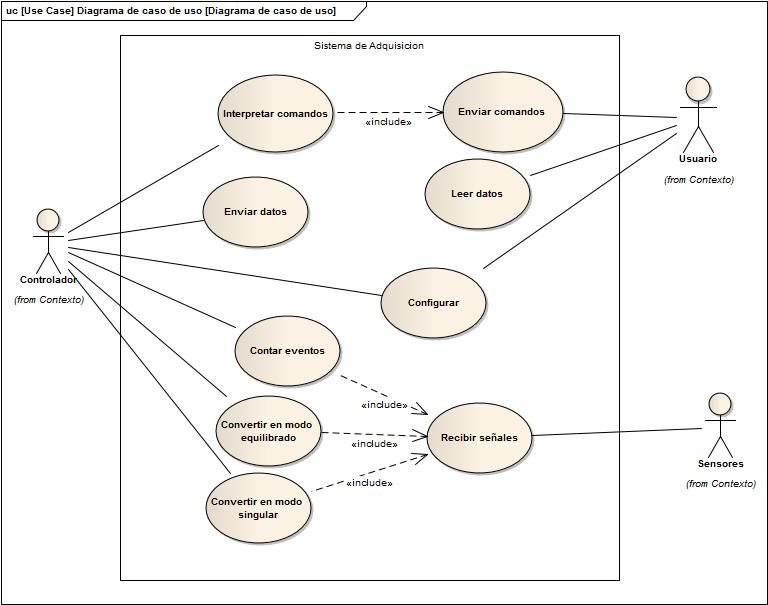
\includegraphics[width=0.80\textwidth, height = 11cm]{casouso1}
  \caption{Diagrama de caso de uso del sistema de medicion e instrumentacion}\label{fig:casouso1}
\end{figure}

El caso de uso ``configurar'' esta generalizado. Las acciones que incluye este caso son:
\begin{itemize}
  \item Configurar la interfaz serial
  \item Configurar canal en modo singular
  \item Configurar canal en modo equilibrado
  \item Configurar contador de eventos
  \item Configurar ganancia del del conversor
  \item Configurar intervalo de medicion para conversion analogica
\end{itemize}

\begin{figure}[h]
  \centering
  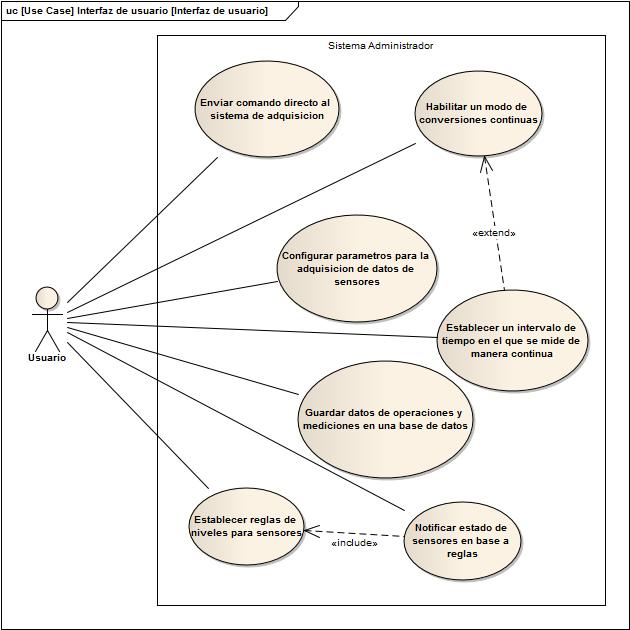
\includegraphics[width=0.80\textwidth, height = 11cm]{casousoAdministrador}
  \caption{Diagrama de caso de uso del sistema administrador}\label{fig:casousoAdministrador}
\end{figure}

En la figura \ref{fig:casouso1}, se puede ver el diagrama de caso de uso para el software a realizar. En cada caso de uso, pueden comenzar a visualizarse las distintas acciones que el programa debe realizar. Al no contar con la posibilidad de organizar el programa en clases, se separo en distintos modulos que agrupan funciones de caracteristicas similares. Estos modulos estan ilustrados como bloques en la figura \ref{fig:bloquesprimeraiteracionsoftware}. Cada bloque correponde a un modulo distinto dentro del programa. Se pueden ver los nombres de cada funcion y el tipo de retorno en cada uno de ellos. Con esto ultimo, damos una idea de las acciones realizadas por las funciones de cada modulo. Una descripcion mas detallada esta en la documentacion del programa \ref{documentacionsoftware}.

\begin{figure}[h]
  \centering
  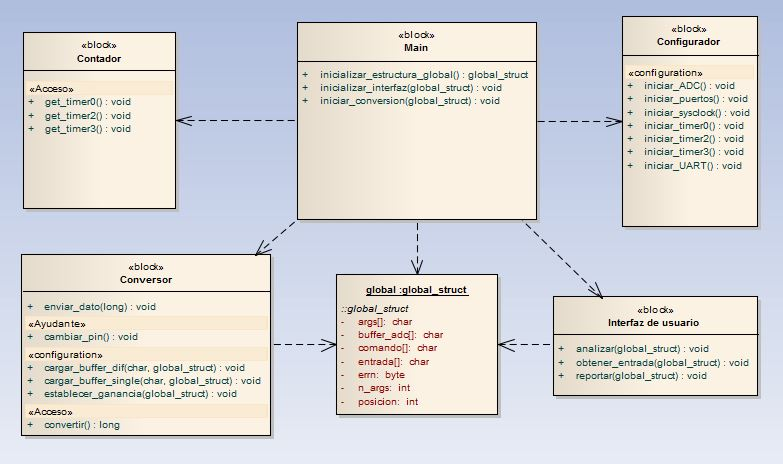
\includegraphics[width=0.80\textwidth, height = 11cm]{bloquesprimeraiteracionsoftware}
  \caption{Diagrama de bloques de la primera iteracion de software}\label{fig:bloquesprimeraiteracionsoftware}
\end{figure}

El objetivo de los diagramas ilustrados es una descripcion grafica del sistema. Es necesario destacar que, desde el principio, la evolucion del programa ocasiono que los diseños de los modulos fueran cambiando. Los cambios fueron debidos a multiples razones: particularidades del funcionamiento del microcontrolador que no se tuvieron en cuenta, limitaciones del entorno, etcetera. En el presente informe, intentamos describir de manera general el funcionamiento del programa, y destacar aquellos cambios que surgieron de problemas imprevistos, y que tuvieron incidencia importante en el sistema.

\begin{itemize}
  \item El \textbf{Main o Bloque Principal} principalmente obtiene los datos de los sensores, los procesa, y los envia al modulo principal. Ademas de esto, configura el funcionamiento del ADC segun los parametros dados por el usuario. El usuario puede elegir la cantidad de pines que va a utilizar como entrada segun la cantidad de sensores que quiera medir, puede elegir un nivel de ganancia de amplificacion de la señal antes de la conversion, y puede tambien elegir el modo de obtencion de los datos (diferencial o single-ended).
  \item El \textbf{Contador} se encarga de obtener los valores en los contadores de eventos.
  \item El \textbf{Interfaz de Usuario} en este modulo se levanta la interfaz con la que interactua el usuario para establecer los parametros configurables del sistema.
  \item El \textbf{Configurador} interactua directamente con el hardware del microcontrolador. Realiza todas las configuraciones necesarias para poder hacer funcionar cada modulo. Inicializa todos los registros pertinentes, el clock del sistema y setea los puertos de entrada y salida.
  \item El \textbf{Serial} envia los datos por interfaz serial. Puede ser UART o $I^{2}$C.
\end{itemize}

% subsection modelos_estaticos (end)

Los fabricantes del microcontrolador proporcionan una libreria en C para trabajar con los registros del procesador. Todos los bloques excepto el de la interfaz grafica, manipulan registros para realizar las distintas acciones que le corresponden segun la funcion que se ejecuta.  


\subsection{Modelos dinamicos} % (fold)
\label{sub:modelos_dinamicos}

Mediante el uso de diagramas de secuencia, explicamos en esta seccion las interacciones entre el usuario y el sistema que cubren los requerimientos principales. Las funciones incolucradas en cada interaccion son las mismas declaradas en el diagrama de bloques del sistema. La mayoria de los flujos que se describen en estos modelos fueron desarrollados iterativamente, es decir, son producto de un desarrollo incremental, hasta llegar a la iteracion actual. La iteracion \ref{cha:iteracion_5} modela las interacciones del programa en su estado final. \\

El objetivo de esta iteracion fue diseñar el programa con un paradigma de configuracion y loop infinito. Es decir, en una etapa inicial, el usuario configura todos los parametros necesarios del sistema, y una vez que se le da arranque, el sistema convierte en modo automatico en un loop infinito, hasta que el usuario le da parada. La figura \ref{secuenciaconfiguracionbasica} muestra una secuencia para realizar una configuracion de un canal del conversor en modo de canal unico. En la figura \ref{fig:secuenciaconversioncontinua}, ilustra como el sistema se coloca en modo de conversion continua, idealmente luego de una configuracion previa. 

\begin{figure}[h]
  \centering
  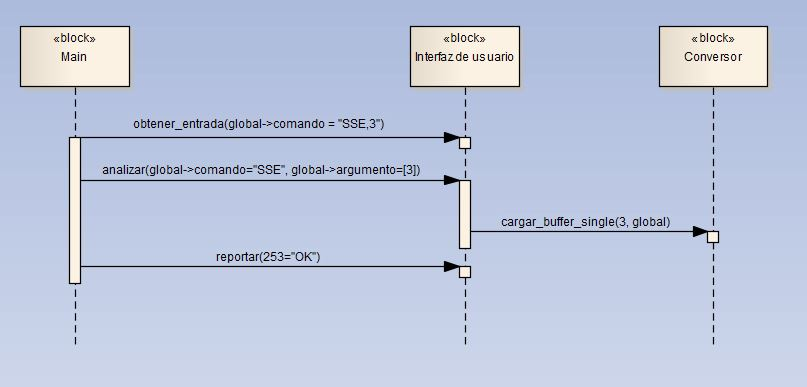
\includegraphics[width=0.80\textwidth, height = 11cm]{secuenciaconfiguracionbasica}
  \caption{Diagrama de secuencia para una configuracion del conversor. Establece el canal 3 en modo canal unico}\label{fig:secuenciaconfiguracionbasica}
\end{figure}

\begin{figure}[h]
  \centering
  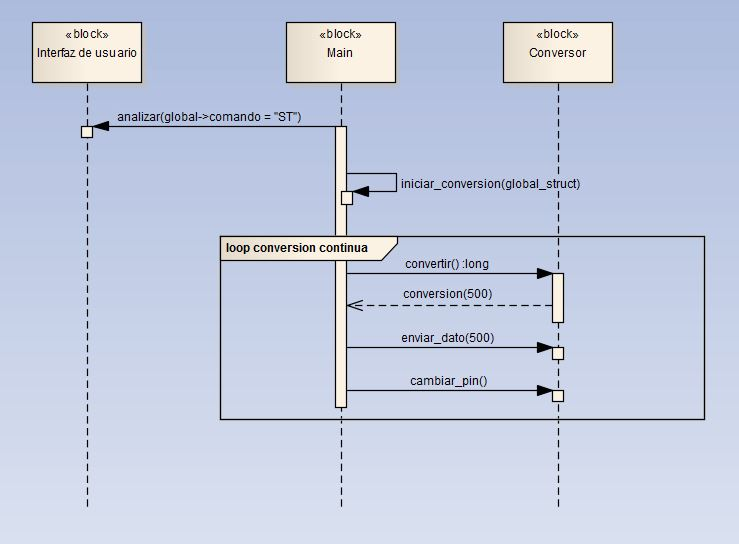
\includegraphics[width=0.80\textwidth, height = 11cm]{secuenciaconversioncontinua}
  \caption{Diagrama de secuencia para la activacion de conversiones en modo continuo luego de una configuracion previa.}\label{fig:secuenciaconversioncontinua}
\end{figure}


\subsection{Logica de las funciones del conversor} % (fold)
\label{sub:logica_de_las_funciones_del_conversor}

Los registros del microcontrolador permiten manipular el conversor de la siguiente manera (para propositos de la logica de conversion):

\begin{itemize}
  \item Se puede establecer de 1 hasta 8 pines en modo canal unico
  \item Se puede establecer de 1 hasta 4 pares de pines en modo diferencial
  \item Se puede establecer un nivel de ganancia de x2 a x128 para todos los canales
\end{itemize}

La logica de las funciones dentro del bloque de software perteneciente al conversor permiten establecer la configuracion del conversor para las mediciones que se quieran hacer. Las funciones que interactuan con el conversor analogico digital o con la logica de conversion de manera directa, son las siguientes (figura \ref{fig:bloquesprimeraiteracionsoftware}):

\begin{itemize}
  \item \textit{convertir}: Interactua con el hardware del microcontrolador para obtener la ultima conversion realizada. Es ejecutada unicamente por la rutina de interrupcion del ADC (iniciada en cada "End of Conversion")
  \item \textit{cargar\_buffer\_single}: carga el buffer de conversion en una posicion que depende de un parametro de entrada, con el numero "1", indicando que el canal que se corresponde con esa posicion en el buffer se debe leer en modo canal unico
  \item \textit{cargar\_buffer\_dif}: carga el buffer de conversion en una posicion que depende de un parametro de entrada, con el numero "2", indicando que el canal que se corresponde con esa posicion en el buffer, y el canal siguiente a ese, deben ser leidos en modo diferencial.
  \item \textit{cambiar\_pin}: Establece el canal por donde se medira la proxima conversion.
\end{itemize}
% subsection modelos_dinamicos (end)

\subsection{Buffer de conversion y logica de cambio de canal en conversion continua} % (fold)
\label{sub:buffer_de_conversion_y_logica_de_cambio_de_canal_en_conversion_continua}

Las funciones \textit{cargar\_buffer\_single} y \textit{cargar\_buffer\_dif}, establecen el modo en el que se leera un canal. Dentro del programa, se crea un buffer de 8 posiciones, cada una representando un canal distinto del ADC. Los valores posibles para estas posiciones son 0, 1 y 2; estos valores representan, respectivamente, que el canal esta o deshabilitado, en modo canal unico o en modo diferencial. Estas funciones, al ser ejecutadas, cargan algun numero en el buffer según que funcion es la que se ejecuto. El buffer se inicializa por defecto en 0, por lo que inicialmente ningun canal esta habilitado para convertir. \\

Cuando se inicia la conversion continua, despues de cada conversion se llama la funcion \textit{cambiar\_pin}. Esta funcion utiliza este buffer para saber cual es el proximo canal a medir. Simplemente maneja un indice que se incrementa hasta 7 y vuelve a 0, recorriendo el buffer cada vez. Segun el numero que tenga la posicion en la que se encuentra, se sabe si debe medirse un canal en modo unico, o el canal y el siguiente en modo diferencial. \\

%Este algoritmo fue el primer prototipo de logica de asignacion y cambio de canal para la lectura de mediciones del conversor. A simple vista es posible ver que los potenciales problemas son muchos. Para empezar, si se asigna el pin 5 en modo canal unico y el modo 4 en modo diferencial, el programa intentara medir en dos modos distintos el mismo canal, dando seguramente resultados inconsistentes. 

% subsection buffer_de_conversion_y_logica_de_cambio_de_canal_en_conversion_continua (end)

% subsection logica_de_las_funciones_del_conversor (end)

\subsection{Logica de las funciones de la interfaz} % (fold)
\label{sub:logica_de_las_funciones_de_la_interfaz}

% Aca es necesario partir el tema en 2.. porque al principio empezamos haciendo todo mal. quisimos hacder una especioe de menu interactivo que le diera la posivilidad al usuario de poder elegir entre distintas opciones de este menu, desplegadas en forma de arbol, para que pudiera elegir la configuracion que quisiera. O sea, arrancaba al principio con un menu general donde ibas navegando hasta poner la configuracion que querias. Asi empezamos, y seguimos con esa logica hasta que se hizo insufrible el programa. Cada vez que queriamos agregar una nueva opcion eran muchas lineas de codigo para cambiar. ahi es cuando investigando me llego el concepto de lo que se llama MMLo "man machine language". Es una logica muy simple. es como un paradigma de interfaz hombre maquina, donde el usuario lo que hace es enviar unos comandos estandarizados y una serie de argumentos, armados en base a una expersion regular. Cisco y Unix Bash usan este paradigma para interactuar con los usuarios. la idea es tan simple como poderosa, lo unico que habia que hacer era decidir como iba a ser el formato de entrada. El analisis posterior es una secuencia que parsea la entrada en busca del comando y los parametros. con el comando, se sabe que funcion ejecutar, y los argumentos son pasados como parametros para esta funcion. Este paradigma es mas complicado de sacar andando, pero es mucho mas escalable que el del menu. a la hora de agregar funcionalidades nuevas se hacia en mucho menos tiempo. Ademas, hace que el programa sea mucho mas facil de testear con unit testing.

La interfaz de usuario tuvo dos implementaciones, siendo la segunda un reemplazo de la primera.

La primera interfaz fue de tipo ``Menu Based Interface'' o interfaz basada en menu, donde las acciones a realizar son ofrecidas por la interfaz y seleccionadas por un usuario. Cada accion esta clasificada segun el grupo de acciones al que pertenezca. Por ejemplo: para configurar el pin 4 del ADC en modo canal unico, es necesario navegar por las opciones del menu de la forma ``configuracion->configurar pin ADC->pin 4->modo canal unico''. Siguiendo este patron de diseño, en cada adicion de una nueva accion, habia que buscar el grupo al que pertenecia y programar la logica necesaria para ejecutar la accion en base a la navegacion del usuario dentro del menu. Esta forma de desarrollo probo ser muy poco escalable, y tuvimos que cambiarla por la dificultad que traia a la hora de agregar nuevas acciones. \\

La segunda interfaz diseñada fue de tipo ``Command line interface''. En este tipo de interfaz, el usuario ingresa un comando y uno o varios argumentos en un formato que respeta una expresion regular. Bajo este concepto, se necesita un parser o analizador de comandos que extraiga de la entrada el comando y los argumentos, y realice acciones segun ellos. En nuestro caso, cada comando representa una funcion distinta de nuestro programa, y los argumentos pasan a ser parametros de la funcion. \\

Luego de implementar un analizador de comandos, agregar funcionalidades al programa fue mas simple y rapido con una interfaz basada en linea de comando que con una basada en menu. Por lo que el primer diseño fue descartado y el segundo se mantuvo.

% subsection logica_de_las_funciones_de_la_interfaz (end)



% section desarrollo (end)

\section{Pruebas} % (fold)
\label{sec:pruebas}


\subsection{Tests unitarios} % (fold)
\label{sub:tests_unitarios}

Cada una de las funciones, tanto si interactuan con el hardware del micro como si no, estan testeadas utilizando unit-testing en C, con ayuda del framework ``minunit''\cite{minunit}. Los unit-tests se ejecutaban de la misma manera que se ejecutaba el programa principal, y corria todos los tests, dando como resultado la cantidad de tests que pasaron y los que fallaron.

% subsection tests_unitarios (end)

\subsection{Tests de sistema} % (fold)
\label{sub:tests_de_sistema}

las pruebas de sistema se realizaron utilizando la placa de desarrollo mencionada en la seccion PONER ACA LA SECCION DONDE HABLAMOS DE LA SILICON LABS. Al no tener todavia una implementacion hecha del sistema, se utilizo esta placa para testear el codigo embebido en el microcontrolador, que en definitiva seria el mismo que iria en la placa a construir

\begin{table}[h]
\centering
\caption{Test de sistema 1}
\label{tab:testsistema1}
\begin{tabular}{
>{\columncolor[HTML]{D3FBFA}}c 
>{\columncolor[HTML]{D3FBFA}}l }
\multicolumn{2}{c}{\cellcolor[HTML]{68CBD0}{\color[HTML]{000000} Prueba de sistema}}                                                                                                                                                                                                                                                   \\
Prueba \#        & 1                                                                                                                                                                                                                                                                                                                   \\
Nombre           & Comportamiento esperado del conversor en modo canal unico                                                                                                                                                                                                                                                           \\
Descripcion      & Se conecta un generador de tension en uno de los canales del conversor y se mide en ese canal en modo canal unico, y de esta forma comprobar no tan solo que se este midiendo, sino ademas que estas mediciones esten calibradas para este modo.                                                                                   \\
Pre-condiciones  & \tabitem Sistema configurado con un pin en modo canal unico \\
                    \tabitem Generador de tension conectado al pin configurado \\
                    \tabitem Computadora conectada al sistema mediante cable serial RS-232 \\
                    \tabitem Lector de canal serial abierto en la computadora \\
                    \tabitem Sistema midiendo en modo de conversiones continuas\\

Post-condiciones & Los datos de las conversiones que aparezcan en el programa lector de interfaz serial en la computadora deberian corresponderse con los valores de tension provenientes del generador                     
\\
Resultados       & Las mediciones dieron resultados coherentes, con algunas variaciones esperadas debido al ruido presente en el ambiente.                                                                                                   
\end{tabular}
\end{table}

\begin{table}[h]
\centering
\caption{Test de sistema 2}
\label{tab:testsistema2}
\begin{tabular}{
>{\columncolor[HTML]{D3FBFA}}c 
>{\columncolor[HTML]{D3FBFA}}l }
\multicolumn{2}{c}{\cellcolor[HTML]{68CBD0}{\color[HTML]{000000} Prueba de sistema}}                                                                                                                                                                                                                                                   \\
Prueba \#        & 2                                                                                                                                                                                                                                                                                                                   \\
Nombre           & Comportamiento esperado del conversor en modo diferencial                                                                                                                                                                                                                                                          \\
Descripcion      & Se conecta un generador de tension en uno de los canales del conversor y se mide en ese canal en modo diferencial, y de esta forma comprobar no tan solo que se este midiendo, sino ademas que estas mediciones esten calibradas para este modo. Ademas, se comprueba el funcionamiento de las mediciones en modo diferencial, intentando medir tensiones negativas.                                                                                  \\
Pre-condiciones  & \tabitem Sistema configurado con un pin en modo diferencial \\
                    \tabitem Generador de tension conectado al par de pines configurados en modo diferencial. Con el borne positivo en uno y masa en el otro\\
                    \tabitem Computadora conectada al sistema mediante cable serial RS-232 \\
                    \tabitem Lector de canal serial abierto en la computadora \\
                    \tabitem Sistema midiendo en modo de conversiones continuas\\

Post-condiciones & Los datos de las conversiones que aparezcan en el lector de interfaz serial en la computadora deberian corresponderse con los valores de tension provenientes del generador  
\\ 
Resultados       & Las mediciones no dieron resultados coherentes. Aunque los cambios en el generador se reproducian en la medicion, los datos no eran los mismos. Esto se debe a que cuando se mide en modo diferencial, el cero pasa a ser la tension de referencia dividida en dos, para representar los valores negativos. La logica del programa no tenia en cuenta esto, y media las tensiones de forma desfasada.                                                                                                                                                     
\end{tabular}
\end{table}

\begin{table}[h]
\centering
\caption{Test de sistema 3}
\label{tab:testsistema3}
\begin{tabular}{
>{\columncolor[HTML]{D3FBFA}}c 
>{\columncolor[HTML]{D3FBFA}}l }
\multicolumn{2}{c}{\cellcolor[HTML]{68CBD0}{\color[HTML]{000000} Prueba de sistema}}                                                                                                                                                                                                                                                   \\
Prueba \#        & 3                                                                                                                                                                                                                                                                                                                   \\
Nombre           & Comportamiento esperado del contador de eventos                                                                                                                                                                                                                                                          \\
Descripcion      & Se conecta un generador de onda cuadrada en una entrada GPIO que pueda servir como entrada a algun contador de eventos. Si el contador esta activo, se deberia poder ver que el numero de cuentas incrementa al ritmo de la frecuencia configurada en el generador                                                                                  \\
Pre-condiciones  & \tabitem Sistema configurado con un contador de eventos activo \\
                    \tabitem Generador de frecuencia conectado al pin configurado como contador. \\
                    \tabitem Computadora conectada al sistema mediante cable serial RS-232 \\
                    \tabitem Lector de canal serial abierto en la computadora \\

Post-condiciones & El contador deberia contar con una frecuencia igual a la del generador de onda cuadrada
\\ 
Resultados       & La cuenta era consistente con la frecuencia del generador.                                                                                                                                                     
\end{tabular}
\end{table}
% subsection tests_de_sistema (end)

% section pruebas (end)
\section{Conclusiones de la iteracion 2} % (fold)
\label{sec:conclusiones_de_la_iteracion_2}


\subsection{Estado de los requerimientos} % (fold)
\label{sub:estado_de_los_requerimientos}


De la seccion \ref{sec:requerimientos_de_la_iteracion}, volvemos a redactar los requerimientos, pero teniendo en cuenta el estado del programa al final de esta iteracion.

\begin{itemize}
\item El programa utiliza el conversor del microcontrolador para transformar señales analogicas de fuentes externas a datos digitales
\item El programa utiliza los contadores del microcontrolador para contar eventos de fuentes externas
\item El programa utiliza el modulo serial UART del microcontrolador para enviar los datos a otra placa o microprocesador
\item No es posible utilizar el modulo SMBus del microcontrolador.
\item Para cada canal del conversor:
\begin{itemize}
\item El usuario puede habilitar o inhabilitar el canal para la medicion
\item El usuario puede configurar el modo de medicion (canal unico o diferencial). En caso de ser canal unico especificarse un solo canal, y dos canales para modo diferencial.
\item No es posible configurar un tiempo de intervalo entre cada medicion
\end{itemize}
\item Para cada contador:
\begin{itemize}
\item El usuario puede habilitar o inhabilitar el conteo de eventos.
\end{itemize}
\item No es posible elegir el protocolo serial para comunicarse con la placa o microprocesador externo que recibira los datos, obligadamente debe usarse UART.

\end{itemize}
% subsection estado_de_los_requerimientos (end)

\subsection{Objetivos para la proxima iteracion} % (fold)
\label{sub:objetivos_para_la_proxima_iteracion}

Teniendo un prototipo de software, lo ideal fue comenzar a pensar en un diseño de hardware en donde hacerlo correr. Por lo que el objetivo de la iteracion 3 fue realizar un diseño de harware para la placa de instrumentacion e implementarlo en un PCB; y una vez construido, realizar pruebas que aseguren el funcionamiento del mismo.

% subsection objetivos_para_la_proxima_iteracion (end)
% section conclusiones_de_la_iteracion_2 (end)
% chapter iteracion_2 (end)

\chapter{Iteracion 3: Primer prototipo de Hardware} % (fold)
\label{cha:iteracion_3}


\section{Introduccion} % (fold)
\label{sec:introduccion}

la primera placa que fue una verga. tenia el rs232, tenia 8 entradas, tenia la alimentacion separada de la entrada para la programacion del micro. osea podia alimentarse mediante el debugger o alimentacion externa. se adapto el diseño de la placa para poder programar el micro con el debugger de silicon labs. hay que tener en cuenta que nos basamos en el diseño hecho por silicon labs de la placa de desarrollo c8051f352 que teniamos en el lac. la vamos a haber construido en esta iteracion, y lo unico que llego a hacer fue conectarse con la ide. nada mas, el resto no anduvo nada. 

% section introduccion (end)

\section{Requerimientos de la iteracion} % (fold)
\label{sec:requerimientos_de_la_iteracion}

Diseñar y construir un prototipo de placa con las siguientes caracteristicas

\begin{itemize}
\item El circuito debe incluir en su diseño aquellos requisitos de hardware impuestos por el mismo microcontrolador(?)
\item Al circuito se le deben poder conectar 8 entradas analogicas.
\item Al circuito se le deben poder conectar 4 entradas de eventos digitales externos.
\item Las entradas analogicas deben tener filtros para mejorar la inmunidad al ruido.
\item Se debe incluir en el diseño el circuito necesario para soportar comunicacion via RS232
\item La placa deberia poder alimentarse a traves de una fuente de tension externa.
\item Se deberia poder conectar el debugger del microcontrolador a la placa para poder programarlo.
\item El circuito de programacion del microcontrolador deberia estar separado la placa principal.
\end{itemize}


% section requerimientos_de_la_iteracion (end)

\section{Desarrollo} % (fold)
\label{sec:desarrollo}

% section desarrollo (end)

\section{Pruebas} % (fold)
\label{sec:pruebas}

% section pruebas (end)

\section{Resultados} % (fold)
\label{sec:resultados}

% section resultados (end)

% chapter iteracion_3 (end)

\chapter{Iteracion 4: Diseño final de hardware} % (fold)
\label{cha:iteracion_4}

\section{Introduccion} % (fold)
\label{sec:introduccion}

El microcontrolador seleccionado contiene 8 entradas para el conversor analogico\-digital. Si se quiere medir en modo diferencial, se tiene una cantidad maxima de 4 canales posibles de entrada. La plataforma de instrumentacion esta pensada para ser utilizada dentro del laboratorio, donde otros proyectos integradores o simplemente academicos la requieran. En la mayoria de los casos, sera necesario que haya un minimo de 8 entradas diferenciales disponibles. \\

Por otro lado, la cantidad de contadores de eventos no llega a ser suficiente, teniendo en cuenta que timer 1 se utiliza para el generador de baudios, y timer 2 y timer comparten la fuente externa de eventos. Esto nos da un total de 2 contadores como maximo, necesitando 4 como minimo. \\

Teniendo en cuenta esto, propusimos agregar un microcontrolador mas a la plataforma, duplicando asi la cantidad de recursos. Agregando este microcontrolador, pasamos a contar con 16 entradas analogicas y 8 contadores, de donde se deduce que son posibles 8 entradas diferenciales, y 4 contadores como maximo. \\

El trabajo a desarrollar en esta iteracion consiste en continuar refinando la construccion de la plataforma, ya que en la iteracion anterior los resultados de las pruebas no dieron como era esperado. Una vez de en la iteracion anterior, dado que su funcionamiento no era el esperado. En esta iteracion, continuamos refinando el trabajo realizado en la iteracion 3, y rediseñamos el PCB para agregar otro microcontrolador.

% section introduccion (end)

\section{Requerimientos de la iteracion} % (fold)
\label{sec:requerimientos_de_la_iteracion}

\begin{itemize}
  \item La placa deberia poder albergar dos microcontroladores C8051f352, con los mismos requerimientos de hardware que en la iteracion 3.
\end{itemize}

% section requerimientos_de_la_iteracion (end)

\section{Desarrollo} % (fold)
\label{sec:desarrollo}

\subsection{Diseño Esquematico}
\label{sub: diseño_esquematico2}

Para simplificar la explicación del diagrama, lo que haremos en esta sección es dividir el circuito entero en subcircuitos mas simples.

\subsubsection{Entradas Analogicas}
\label{subsub: entradas_analogicas2}

Las entradas analogicas con sus filtros se mantuvieron exactamente igual que en el diseño de la primera placa. Para cada una de las entradas se le colocaria un filtro pasa-bajo RC como se muestra en la figura \ref{fig:esquematicoFiltro}.

Mostramos en la figura \ref{fig:esquematicoFiltro2} como quedan todas las entradas analógicas de un solo chip (en el otro es exactamente igual), podemos ver 8 entradas analogicas, cada una con su respectivo filtro. Ademas podemos observar 2 pines llamados PINHD\_AGND\_2, son dos accesos a la masa digital para aquellos sensores que necesiten estar referenciado a masa (colocamos dos masa analogicas para cada uno de los chips).

Del lado derecho del microcontrolador hay dos entradas denominadas VREF+ y VREF-, que nos sirven para manejar los niveles de tension de referencia para la conversion que usara el ADC.

\begin{figure}[H]
\centering
  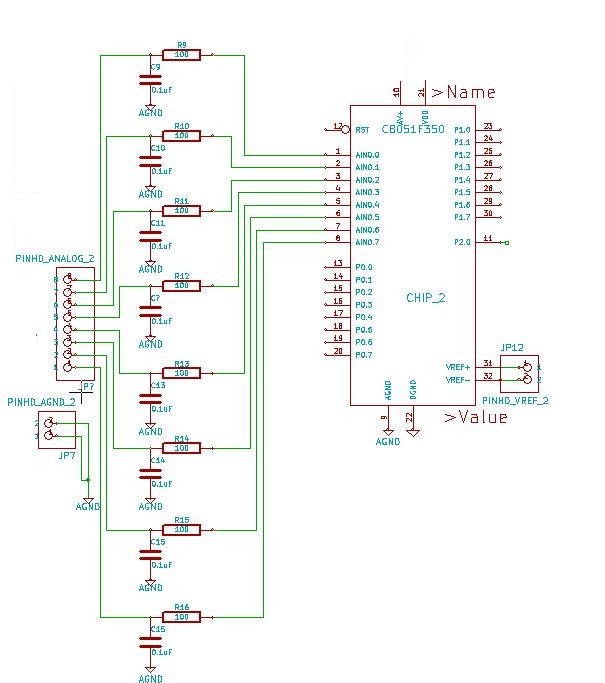
\includegraphics[width=1.10\textwidth, height = 9cm]{esquematicoFiltro2}
  \caption{Esquemático del Circuito Completo de entradas analogicas.}\label{fig:esquematicoFiltro2}
\end{figure}

% subsubsection entradas_analogicas2 (end)

\subsubsection{Circuito de entradas Digitales}
\label{subsub:entradas_digitales}

Como podemos ver en la figura \ref{fig:esquematicoDigital2} colocamos 16 entradas/salidas digitales para el microcontrolador. Cada chip tiene las mismas 16 entradas.

\begin{figure}  [H]
\centering
  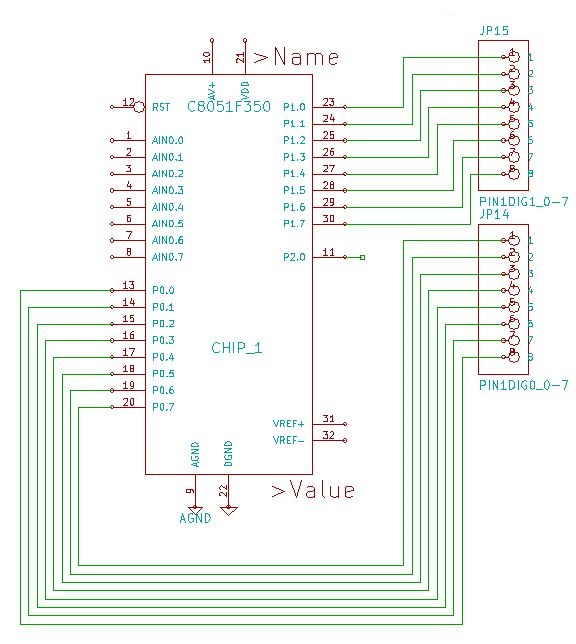
\includegraphics[width=1.0\textwidth, height = 10cm]{esquematicoDigital2}
  \caption{Esquemático del Circuito Completo de entradas/salidas digitales.}\label{fig:esquematicoDigital2}
\end{figure}


% subsubsection entradas_digitales (end)

\subsubsection{Circuito Salida Serial}
\label{subsub:salida_serial2}

La idea de tener una placa a la que se conecten varios sensores analógicos y digitales es que se pueda colocar el lugares remotos, por lo que decidimos que la salida serial deje de ser RS-232 y colocarle dos salidas seriales nivel TTL con un RX y un TX para cada microcontrolador, ademas colocando éste tipo de salida se ahorra mucho espacio, así pudimos reducir el tamaño de la placa. Las salidas seriales se encuentran conectadas directamente en los pines de salidas dijitales P0.4 (Tx) y P0.5(Rx).

% subsubsection salida_serial2 (end)

\subsubsection{Circuito para Debugger y Programación} % (fold)
\label{subsub:debugger_programacion2}

Para programar cada uno de los microcontroladores en principio se penso en colocar dos entradas para el debugger de SiliconLabs, pero nos consumia mucho espacio y el cambio para programar uno y otro se hubiera hecho molesto. Por lo que decidimos poner uno solo, y utilizarlo para los dos microcontroladores, con un jumper de tres pines, para tener la opcion de elegir que micro programar.
En la figura \ref{fig:esquematicoDebugger2} vemos en uno de los C8051f352 como queda conectado el modulo de debugger/programacion.

\begin{figure}  [H]
\centering
  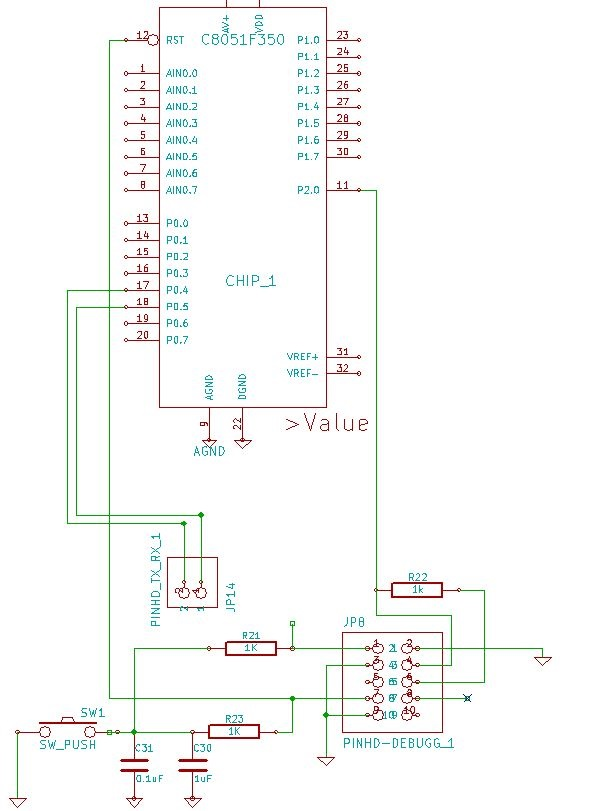
\includegraphics[width=1.0\textwidth, height = 8cm]{esquematicoDebugger2}
  \caption{Esquemático del Circuito para la programacion de los microcontroladores de la placa.}\label{fig:esquematicoDebugger2}
\end{figure}


% subssubection debugger_programacion2 (end)

\subsubsection{Circuito de Potencia}
\label{subsub: circuito_potencia2}

Para el circuito de potencia hicimos lo mismo que con el debugger, colocamos una sola entrada y un solo regulador para toda la placa y alimentar asi los dos microcontroladores. Tambien colocamos un jumpers (JMP3), se utiliza para decidir si alimentamos la placa con una fuente externa o con el debugger/programador de SiliconLabs. 
Sabemos que el principal problema de un sitema embebido es su consumo de energia, por lo que colocamos dos jumpers más, uno para cada una de las entradas de alimentación del segundo microcontroladore (JP4 AV+ y JP5 para VDD). Entonces así podemos elegir desconectar un chip y ahorrar el consumo de energia que este provocaría. 

En la figura \ref{fig:esquematicoPotencia2} se muestra como queda el esquematico del circuito de potencia.

\begin{figure}[H] 
\centering
  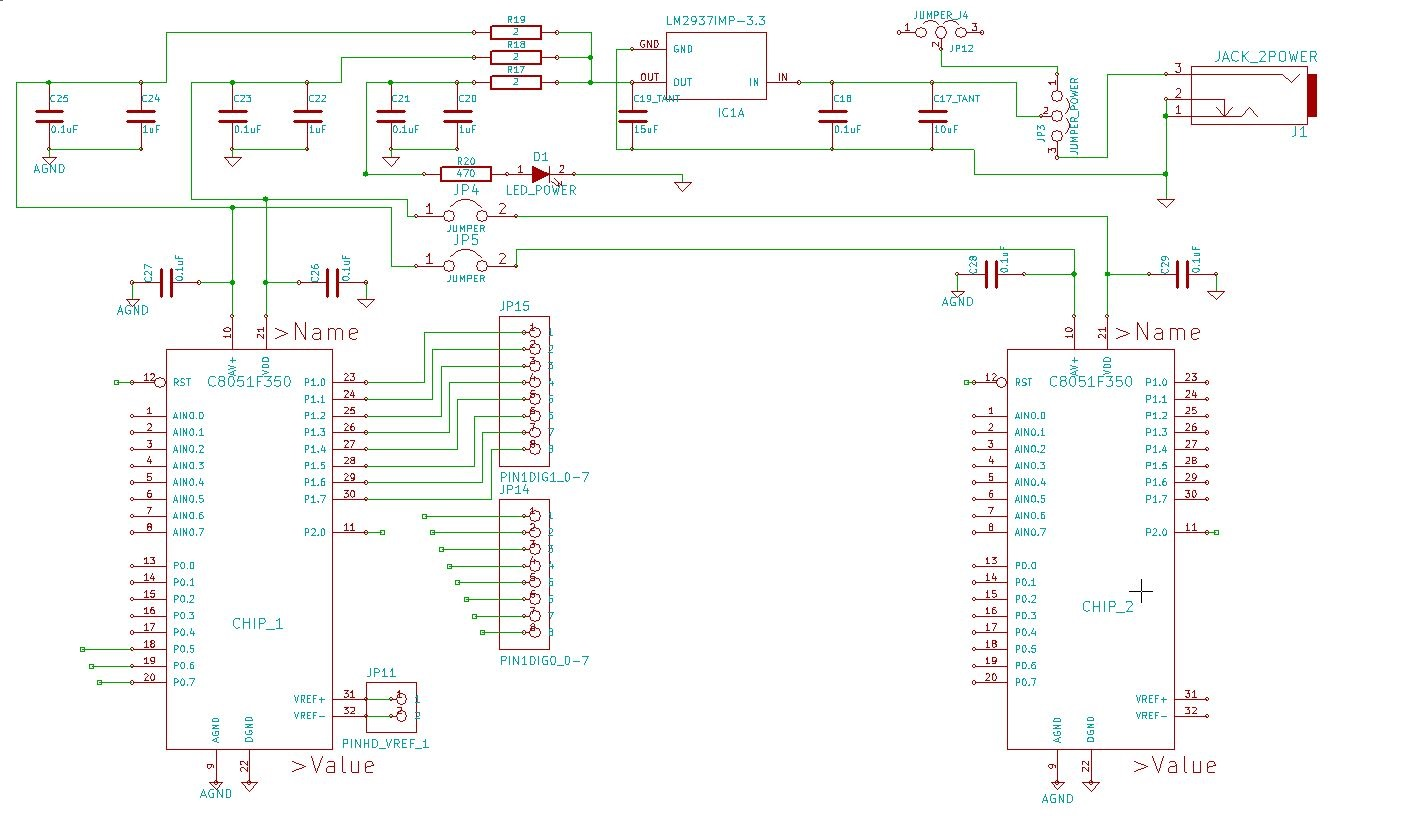
\includegraphics[width=1.0\textwidth, height = 10cm]{esquematicoPotencia2}
  \caption{Esquemático del Circuit para la potencia de alimentación.}\label{fig:esquematicoPotencia2}
\end{figure}

%subsubsection circuito_potencia2 (end)

\subsubsection{Diagrama Esquematico Completo}
\label{subsubsection: esquematico_completo2}

En la figura \ref{fig:esquematicoCompleto2} podemos ver como queda el esquematico entero con los dos microcontroladores y todos los subcircuitos que componen la placa.

\begin{figure}  
\centering
  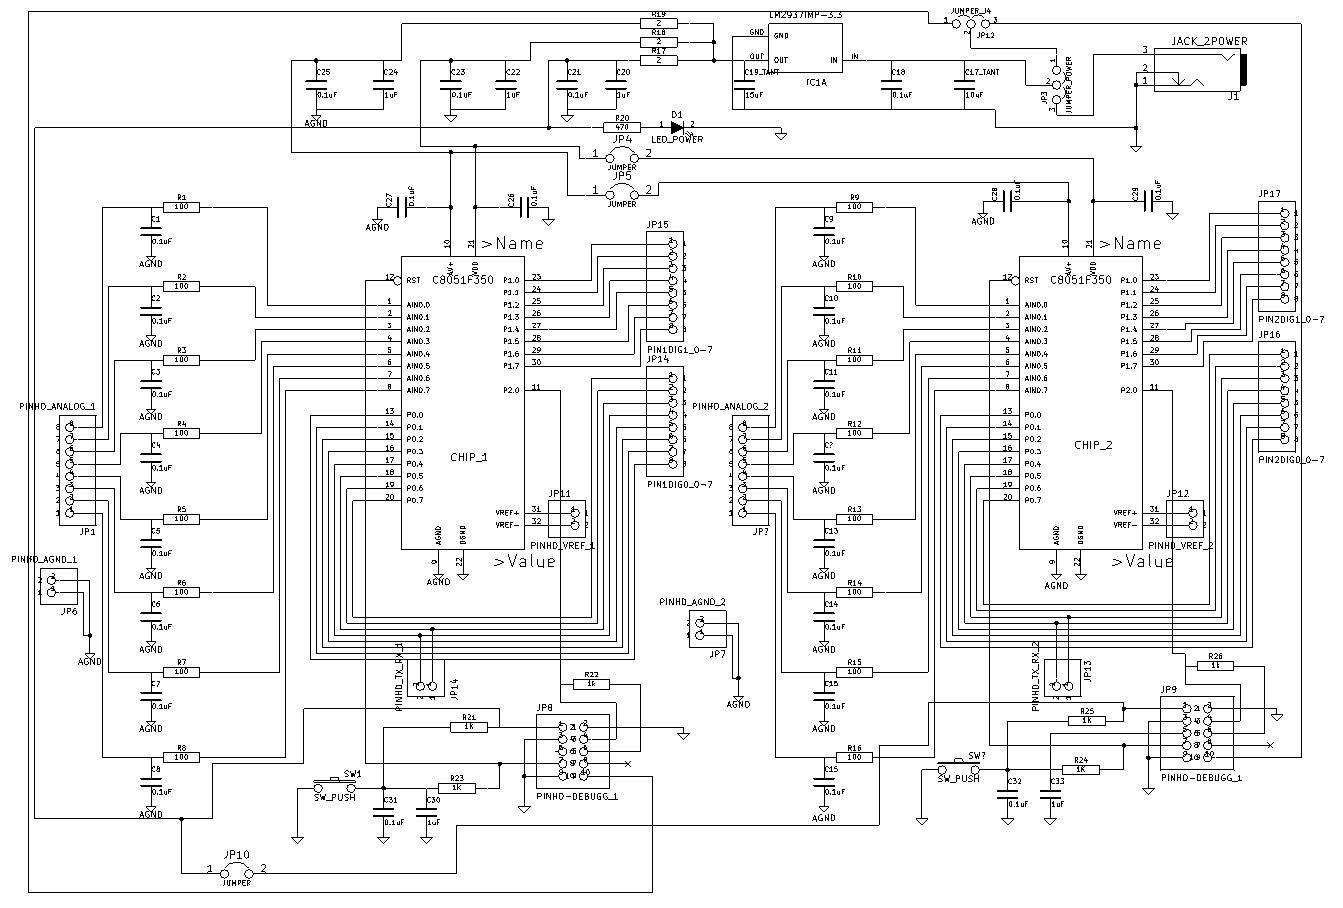
\includegraphics[width=1.10\textwidth, height = 12cm]{esquematicoCompleto2}
  \caption{Esquemático del Circuit completo de la Placa de desarrollo.}\label{fig:esquematicoCompleto2}
\end{figure}


% subsubsection esquematico_completo2 (end)

% subsection diseño_esquematico2 (end)

\subsection{Diseño de Plaqueta de Circuito Impreso (PCB)}
\label{ subsection: diseño_pcb2}

Como esta nueva version de la placa fue diseñada para ser doble capa, se mostrarán 2 figuras, una para la capa superior y otra para la capa inferior. 
A ambas capaz le tuvimos que dividir las masas, en una seccion analogica y una digital, la masa analogica de la capa superior con la de la capa inferior deben estar interconectadas, lo mismo pasa con la masa digital. Por lo que realizamos un drill (un hueco) para que las masas esten en contacto.
En la figura \ref{fig:PCB2a} podemos ver como queda el diagrama PCB de capa superior o frontal, y en la figura \ref{fig:PCB23Da} vemos la misma capa con el visualizador 3D del KiCad.

\begin{figure}[H]
\centering
  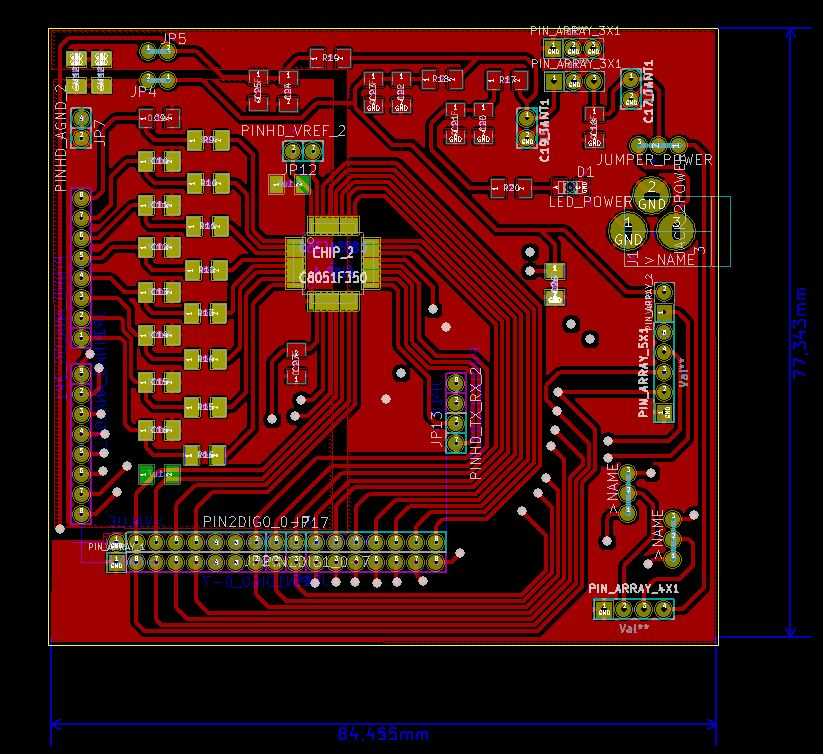
\includegraphics[width=1.0\textwidth, height = 8cm]{PCB2a}
  \caption{Diseño PCB de la capa frontal de la placa.}\label{fig:PCB2a}
\end{figure}

\begin{figure}  [H]
\centering
  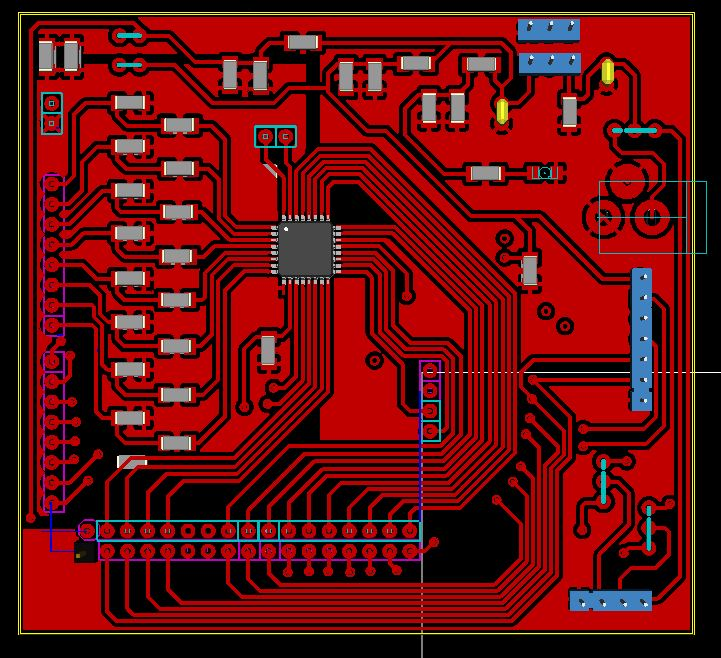
\includegraphics[width=1.0\textwidth, height = 8cm]{PCB23Da}
  \caption{Diseño PCB de la capa frontal de la placa en 3D.}\label{fig:PCB23Da}
\end{figure}

En la figura \ref{fig:PCB2b} podemos ver como queda el diagrama PCB de capa inferior o posterior, y en la figura \ref{fig:PCB23Db} vemos la misma capa con el visualizador 3D del KiCad.

\begin{figure}[H] 
\centering
  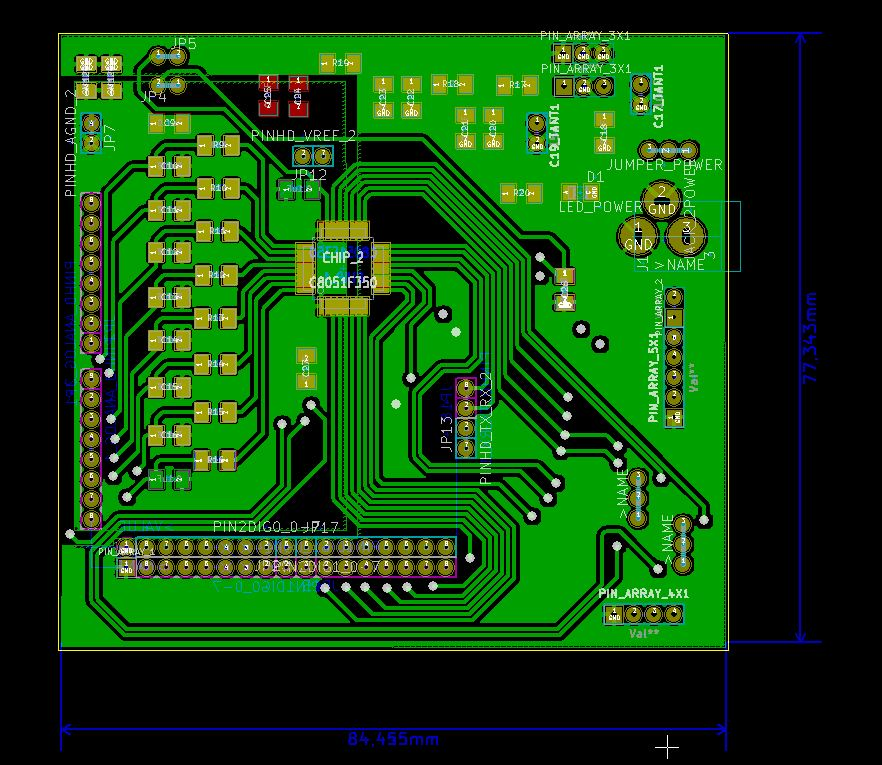
\includegraphics[width=1.0\textwidth, height = 8cm]{PCB2b}
  \caption{Diseño PCB de la capa posterior de la placa.}\label{fig:PCB2b}
\end{figure}

\begin{figure}  [H]
\centering
  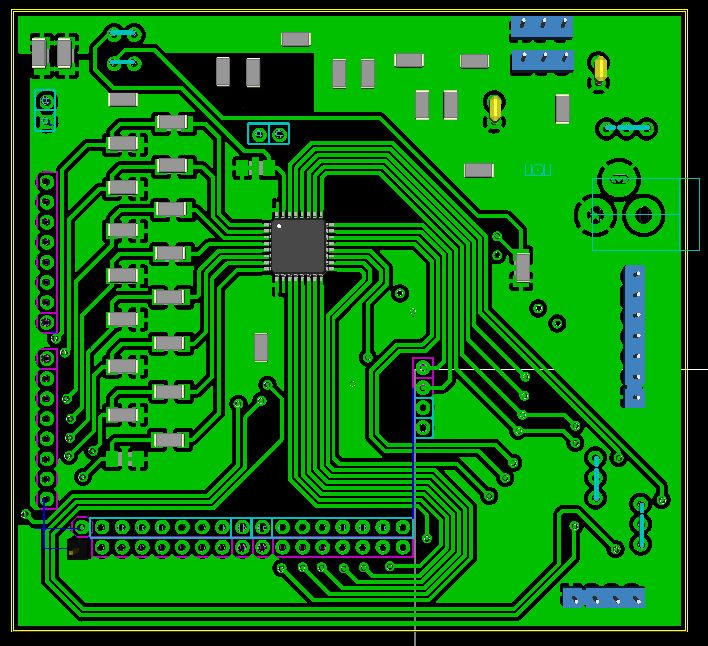
\includegraphics[width=1.0\textwidth, height = 8cm]{PCB23Db}
  \caption{Diseño PCB de la capa posterior de la placa en 3D.}\label{fig:PCB23Db}
\end{figure}


% subsection diseño_pcb2 (end)

\section{Pruebas} % (fold)
\label{sec:pruebas}

En la tabla de pruebas se veran repetidos los mismos tests que en la iteracion anterior, ya que fue necesario que los realicemos nuevamente. La diferencia se encuentran en los resultados.

\begin{table}[h]
\caption{Test de sistema 1}
\label{it4:tab:testsistema1}
\begin{tabular}{p{2cm} p{9cm}}
\multicolumn{2}{c}{\cellcolor[HTML]{68CBD0}{\color[HTML]{000000} Prueba de sistema}} \\
Prueba \#        & 1 \\
\hline
Nombre           & Correcto Diseño de PCB. \\
\hline
Requerimientos  &  \tabitem La placa debe tener dos microcontroladores C8051f352. \\
                &  \tabitem La placa debe tener 16 entradas analogicas. \\
                &  \tabitem La placa debe tener 32 entradas digitales. \\
                &  \tabitem La placa debe tener 2 salidas seriales.   \\
\hline
Descripción      & Se chequea si existen errores en el diseño utilizando el ERC (perfom design rules check) que provee KiCad. \\
\hline
Pre-condiciones  & \tabitem Componentes colocados y ruteados. \\
                 & \tabitem Pads numerados con sus etiquetas.  \\
\hline
Post-condiciones & El resultado de ERC debe ser cero. \\
\hline
Resultados       & No encontramos errores de diseño en el PCB. \\                                                                           
\end{tabular}
\end{table}

\begin{table}[h]
\caption{Test de sistema 2}
\label{it4:tab:testsistema2}
\begin{tabular}{p{2cm} p{9cm}}
\multicolumn{2}{c}{\cellcolor[HTML]{68CBD0}{\color[HTML]{000000} Prueba de sistema}} \\
Prueba \#        & 2 \\
\hline
Nombre           & Correcta impresión de la placa.   \\

\hline
Requerimientos &    \tabitem La placa debe tener dos microcontroladores C8051f352. \\
               &    \tabitem La placa debe tener 16 entradas analogicas.\\
               &    \tabitem La placa debe tener 32 entradas digitales. \\
               &    \tabitem La placa debe tener 2 salidas seriales.    \\
\hline
Descripción      & Corroboramos que todas las pistas y que todos los drills se hayan impreso. Luego con un multimetro seteado en continuidad comprobamos que no existan cortocircuitos entre pistas y masa o entre pads y masa. \\
\hline
Pre-condiciones  & \tabitem Placa impresa. \\
                 & \tabitem Multímetro seteado en continuidad. \\
\hline
Post-condiciones & La placa debe tener las mismas pistas que aparecen en el diseño de PCB, y al medir con el tester nunca debe dar continuidad entre masa y pistas, o entre pads y pistas. \\ 
\hline
Resultados       & Todas las pistas estaban de acuerdo con el PCB. Al medir la continuidad de las pistas no se encontraron a cortocircuitos. \\                                                                                                                                     
\end{tabular}
\end{table}

\begin{table}[h]
\centering
\caption{Test de sistema 3}
\label{it4:tab:testsistema3}
\begin{tabular}{p{2cm} p{9cm}}
\multicolumn{2}{c}{\cellcolor[HTML]{68CBD0}{\color[HTML]{000000} Prueba de sistema}} \\
Prueba \#        & 3 \\
\hline
Nombre           & Correcta soldadura de Componentes. \\
\hline
Requerimientos &    \tabitem La placa debe tener dos microcontroladores C8051f352. \\
               &    \tabitem La placa debe tener 16 entradas analogicas. \\
               &    \tabitem La placa debe tener 32 entradas digitales. \\
               &    \tabitem La placa debe tener 2 salidas seriales.      \\
\hline
Descripción      & Se utiliza el multimetro seteado en continuidad para poder chequear si existen cortocircuitos y para saber si todos los componentes estan bien interconectados. \\
\hline
Pre-condiciones  & \tabitem Placa impresa. \\
                 & \tabitem Pistas impresas correctamente. \\
                 & \tabitem Componentes soldados. \\
                 & \tabitem Multimetro seteado en continuidad. \\
\hline
Post-condiciones &  No deben encontrarse cortocircuitos, y deben comprobarse la continuidad de las interconexiones de componentes. \\ 
\hline
Resultados       & Encontramos cortocircuitos luego de soldar los componentes, se solucionaron desoldando y volviendo a soldar los componentes. \\                                                                                                                                             
\end{tabular}
\end{table}

\begin{table}[h]
\centering
\caption{Test de sistema 4}
\label{it4:tab:testsistema4}
\begin{tabular}{p{2cm} p{9cm}}
\multicolumn{2}{c}{\cellcolor[HTML]{68CBD0}{\color[HTML]{000000} Prueba de sistema}} \\
Prueba \#        & 4 \\
\hline
Nombre           & Correcta Comunicación Con IDE SiliconLabs. \\
\hline
Requerimientos &  \tabitem Se debería poder conectar el debugger del microcontrolador a la placa para poder programarlo. \\
\hline
Descripción      & Se utilizo el cable USB con el debugger de SiliconLabs para conectar la placa a la PC. \\
\hline
Pre-condiciones  & \tabitem Placa impresa. \\
                 & \tabitem Pistas impresas correctamente. \\
                 & \tabitem Componentes soldados. \\
                 & \tabitem IDE SiliconLabs instalada en la PC. \\
\hline
Post-condiciones &  Al abrir la IDE y apretar el botón de "Connect" el programa debe reconocer el tipo de microcontrolador al que esta conectado. \\ 
\hline
Resultados       &  Conectamos la placa a la PC y en la IDE apretamos el botón de conectar, con lo que nos reconoció que el micro que se había conectado fue un C8051f352.     \\                                                                                                                                               
\end{tabular}
\end{table}

\begin{table}[h]
\centering
\caption{Test de sistema 5}
\label{it4:tab:testsistema5}
\begin{tabular}{p{2cm} p{9cm}}
\multicolumn{2}{c}{\cellcolor[HTML]{68CBD0}{\color[HTML]{000000} Prueba de sistema}} \\
Prueba \#        & 4 \\
\hline
Nombre           & Correcta programacion del microcontrolador. \\
\hline
Requerimientos &  \tabitem Se debería poder conectar el debugger del microcontrolador a la placa para poder programarlo. \\                                   
\hline
Descripción      & Se utilizo el cable USB con el debugger de SiliconLabs para conectar la placa a la PC y descargarle un programa .hex al microcontrolador. \\
\hline
Pre-condiciones  & \tabitem Placa impresa. \\
                 & \tabitem Pistas impresas correctamente. \\
                 & \tabitem Componentes soldados. \\
                 & \tabitem IDE SiliconLabs instalada en la PC. \\
                 & \tabitem IDE SiliconLabs reconociendo el C8051f352. \\
\hline
Post-condiciones &  Al abrir la IDE y apretar el botón de "Connect" el programa debe reconocer el tipo de microcontrolador al que esta conectado y luego a traves de la misma IDE o del "Flash Programing Utilitys" cargarle un proframa .hex al c8051f352. \\ 
\hline
Resultados       &  Conectamos la placa a la PC y desde el "Flash Programing Utilitys" se pudo cargar un programa a los microcontroladores soldados en la placa. \\                                                                                                  
\end{tabular}
\end{table}

\begin{table}[h]
\centering
\caption{Test de sistema 6}
\label{it4:tab:testsistema6}
\begin{tabular}{p{2cm} p{9cm}}
\multicolumn{2}{c}{\cellcolor[HTML]{68CBD0}{\color[HTML]{000000} Prueba de sistema}} \\
Prueba \#        & 4 \\
\hline
Nombre           & Correcta funcionamiento de las entradas analogicas y salidas digitales. \\                      

\hline
Requerimientos &    \tabitem La placa debe tener dos microcontroladores C8051f352. \\
               &    \tabitem La placa debe tener 32 entradas digitales. \\
               &    \tabitem La placa debe tener 16 entradas analogicas. \\
\hline
Descripción      & Cargamos un programa a los microcontroladores con el que medimos una entrada analogica proveniente de una fuente (prestada en el Pañol) y utilizamos el ADC para poder transformar esa señal analogica en digital, luego en una de las salidas/entradas digitales se conecto un led, el cual titilaria con mayor frecuencia a medida que se aumenta el voltage que entrega la fuente utilizada. \\
\hline
Pre-condiciones  & \tabitem Placa impresa. \\
                 & \tabitem Pistas impresas correctamente. \\
                 & \tabitem Componentes soldados. \\
                 & \tabitem IDE SiliconLabs instalada en la PC. \\
                 & \tabitem IDE SiliconLabs reconociendo el C8051f352. \\
                 & \tabitem Programa de prueba correctamente cargado en el C8051f352. \\
                 & \tabitem Fuente de Tension externa conecectada a las entradas analogicas con referencia en masa analogica. \\
                 & \tabitem Resistencia conectada en serie con un Led a una salida digital del C8051f352. \\
\hline
Post-condiciones &  Al apregar el boton de "Go" en el "Flash Programing Utilitys" para que arranque a funcionar el programa cargado en el microcontrolador debe titilar el led variando su frecuencia en directa relacion con la variacion de la tension de la fuente conectada a las entradas analogicas. \\ 
\hline
Resultados       &  Cargamos el programa en el microcontrolador, y con todas las pre-condiciones cumplidas hicimos correr el programa. El led efectivamente vario su frecuencia de prendido y apagado a medida que aumentabamos o disminuiamos la tension que entregaba la fuente externa. \\                                                                                                            
\end{tabular}
\end{table}


% section pruebas (end)

\section{Resultados} % (fold)
\label{sec:resultados}

Cumplimos con los requerimientos planteados para esta iteracion:

\begin{itemize}
  \item La placa debe tener dos microcontroladores C8051f352.
  \item La placa debe tener 16 entradas analogicas.
  \item La placa debe tener 32 entradas digitales.
  \item La placa debe tener 2 salidas seriales. 
  \item Se debería poder conectar el debugger del microcontrolador a la placa para poder programarlo.
\end{itemize}


 Obtivimos una placa de desarrollo que dobla en recursos a la placa de la iteración anterior. La placa quedó totalmente funcional.
En la figura \ref{fig:} y \ref{fig:} podemos ver como quedo la placa tanto de la capa superior como de la inferior. Lo que observamos es que todos los pines y modulos que se pueden utilizar para conectar alguna interfaz/cable quedaron en la capa frontal, por una cuestion de comodidad al momento de utilizarla.

"AGREGAAAAAAAAAAAAAAAAAR LAS FOTTTOOOOOOOOOOOOOOOOOOOOOOOOOOOOOOOOOOOOOOOOOOOOOOOOOOOOOOOOOOS"

% section resultados (end)

% chapter iteracion_4 (end)

\chapter{Iteracion 5: Diseño final del Software} % (fold)
\label{cha:iteracion_5}

\section{Introduccion} % (fold)
\label{it5:sec:introduccion}

En este capitulo, se describe el desarrollo de la segunda itearacion de software. Hasta el momento, teniamos un programa embebido en el microcontrolador que cumplia con los requerimientos especificados en la seccion \ref{it2:sub:estado_de_los_requerimientos}. En esta iteracion, el objetivo principal es obtener un prototipo final del programa, que cumpla, en lo posible, con todos los requerimientos, priorizando aquellos de mayor riesgo.

% section introduccion (end)

\subsection{Objetivos} % (fold)
\label{it5:ssec:objetivos}

\begin{itemize}
  \item Tener un prototipo final del programa comenzado en la iteracion 2
  \item Tener todo el programa testeado mediante Unit-Testing y tests de sistema.
\end{itemize}

% subsection objetivos (end)

\section{Requerimientos de la iteracion} % (fold)
\label{it5:sec:requerimientos_de_la_iteracion}

Los requerimientos de esta iteracion estan planteados en base a los resultados de las pruebas y el desarrollo de la iteracion 2. 

\begin{itemize}
\item Se deberian poder configurar tiempos de intervalo entre cada medicion para cada canal por separado
\item Se deberian poder guardar las configuraciones actuales en la memoria flash del microcontrolador, para poder reestablecerlas en caso que el sistema se apague y se vuelva a prender.
\item Se deberia generar una marca de tiempo relativa al inicio de conversiones en cada medicion realizada.
\item Los datos que se envian a la placa de gestion para cada medicion deberia inculir, ademas de la medicion, el numero de pin o pines (si es modo diferencial) de donde se esta midiendo. 
\item Los datos que se envian a la placa de gestion para cada medicion deberia inculir, ademas de la medicion, el modo de conversion del canal por donde se esta midiendo.
\item Los datos que se envian a la placa de gestion para cada medicion deberia inculir, ademas de la medicion, la marca de tiempo relativa correspondiente de la medicion hecha. 
\end{itemize}


% section requerimientos_de_la_iteracion (end)

\section{Desarrollo} % (fold)
\label{it5:sec:desarrollo}

Focalizamos el desarrollo del programa en el objetivo de obtener un prototipo final, listo para dejar andando en la placa de instrumentacion construida. En una primera instancia, terminamos aquellas funcionalidades ligadas a los requerimientos principales, y luego nos dedicamos a comprobar el funcionamiento del mismo, mediante unit-testing y tests de sistema.

La figura \ref{fig:bloquesquintaiteracion} muestra el diagrama de bloques del programa para esta iteracion. Con respecto al diagrama en la figura \ref{bloquesprimeraiteracionsoftware}, el cambio mas significativo no es en la estructura, sino que son las funciones dentro de los bloques lo que mas cambio. Hay funciones nuevas, funciones que sufrieron cambios y funciones que se eliminaron. La idea de esta seccion es describir cada una, con el proposito de que se entienda la logica del programa a un nivel general.

\begin{figure}[h]
  \centering
  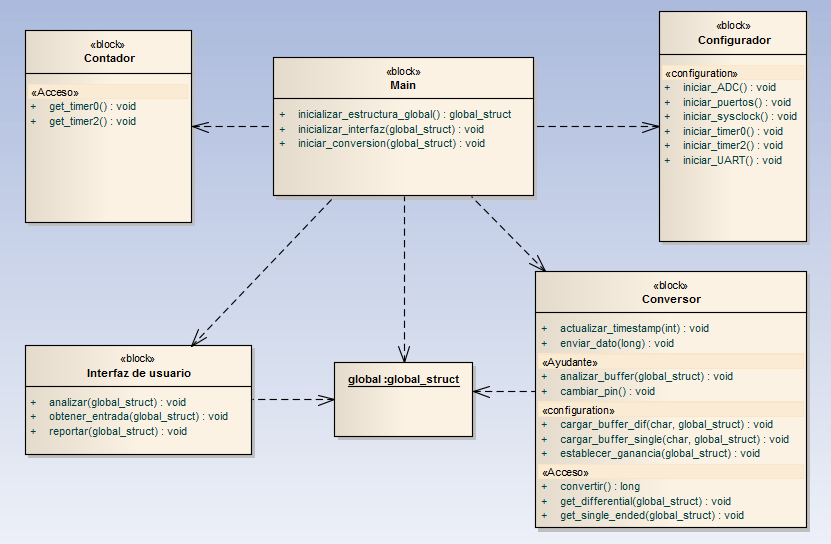
\includegraphics[width=0.80\textwidth, height = 9cm]{bloquesquintaiteracion}
  \caption{}\label{fig:bloquesquintaiteracion}
\end{figure}

\subsection{Conversor} % (fold)
\label{sub:conversor}

Las funciones del conversor se rediseñaron con el objetivo de lograr que el usuario pueda configurar tiempos de intervalos de mediciones en cada canal por separado.

En la seccion \ref{sub:logica_de_las_funciones_del_conversor}, se explica el funcionamiento del buffer del conversor. Hasta el momento, el buffer poseia 8 posiciones, una por cada canal, con el objetivo de informar al programa el estado de ese canal. Estos estados son: inhabilitado, canal unico, o canal diferencial.

\begin{figure}[h]
  \centering
  \includegraphics[width=0.80\textwidth, height = 7cm]{bufferdinamicovacio}
  \caption{Estado de los buffers en el momento en que se terminaron de configurar las distintas vias de conversion, pero aun no se activo el modo de conversion continua}\label{fig:bufferdinamicovacio}
\end{figure}

En esta version del programa, utilizamos dos buffers de 11 posiciones cada uno. A diferencia del buffer de conversion de la iteracion 2, cada posicion ya no representa un unico canal sino que representa una "via de conversion". Una via de conversion es una fuente de telemetria que puede provenir de un canal unico o diferencial.
De manera figurativa, podria decirse que un buffer es "dinamico", y el otro es "estatico". Similar al buffer de conversion de la iteracion 2, el buffer estatico determina si un canal esta habilitado o no. Ademas de esto, determina el valor del intervalo de mediciones de dicho canal. Si la posicion que corresponde a ese canal contiene un 0, el canal esta inhabilitado; cualquier numero mayor a 0 indica que el canal esta habilitado. Si el canal esta habilitado, el numero puede estar en un rango de 1 a 65536, siendo este numero una medida del intervalo temporal que habra entre cada medicion cuando el sistema entre en modo de conversiones continuas. Mientras mayor es el numero, mayor es el intervalo entre cada medicion para ese canal.
A diferencia del buffer original, el modo de conversion ya no se identifica con un numero, sino con la posicion dentro del buffer, ya sea el estatico o el dinamico. Las posiciones del 0 al 7 estan reservadas para los 8 canales del conversor en modo canal unico, y las posiciones del 8 al 11 son para los canales en modo diferencial. Las posiciones 8,9,10 y 11 representan a los pares de pines en modo diferencial (1,2); (3,4); (5,6) y (7,8) respectivamente. 


La secuencia para las conversiones funciona de la siguiente manera:

\begin{enumerate}
\item Cuando se configura el buffer, se establecen las vias de conversion con sus respectivos intervalos poniendo numeros de 1 a 65536 en los elementos del buffer estatico.
\item Cuando se activa el modo de conversiones continuas, se realiza una copia del buffer estatico para obtener el buffer dinamico, que es en realidad una instancia del buffer estatico al comienzo de la conversiones continuas.
\item El programa itera sobre el buffer dinamico, decrementando los valores de cada elemento del buffer que no contenga un 0
\item Cuando se encuentra sobre un elemento que tiene valor igual a 1, es momento de obtener una medicion de la via de conversion ligada a esa posicion.
\item Una vez habilitada la conversion para el canal, se copia el valor que se encuentra en el buffer estatico para la misma posicion en el buffer dinamico. Reiniciando la cuenta.
\end{enumerate}

La funcion que realiza la conversion, es ejecutada cada vez que se encuentra un 1 en una posicion del buffer dinamico. Con el numero de posicion del buffer, se sabe el numero de la via de conversion por donde hay que convertir. Esta via de conversion, como mencionamos anteriormente, puede ser de 0 a 11. En cada numero, se mide lo siguiente:

\begin{itemize}
\item 0 \textrightarrow  canal 0 modo unico
\item 1 \textrightarrow  canal 1 modo unico
\item 2 \textrightarrow  canal 2 modo unico
\item 3 \textrightarrow  canal 3 modo unico
\item 4 \textrightarrow  canal 4 modo unico
\item 5 \textrightarrow  canal 5 modo unico
\item 6 \textrightarrow  canal 6 modo unico
\item 7 \textrightarrow  canal 7 modo unico
\item 8 \textrightarrow  canal 0,1 modo diferencial
\item 9 \textrightarrow  canal 1,2 modo diferencial
\item 10 \textrightarrow  canal 2,3 modo diferencial
\item 11 \textrightarrow  canal 3,4 modo diferencial
\end{itemize}

Se tomaron las medidas suficientes, dentro del programa, para no permitir al usuario que establezca una configuracion donde provoque que se solapen las vias de conversion con respecto a los canales. 

\begin{figure}[h]
  \centering
  \includegraphics[width=0.80\textwidth, height = 7cm]{bufferdinamicolleno}
  \caption{Estado de los buffers en el momento que se activa la conversion continua. Cada vez que un valor del buffer dinamico llega a 1, se reestablece usando el buffer estatico como referencia.}\label{fig:bufferdinamicolleno}
\end{figure}

El numero dentro de cada posicion representa el tiempo del intervalo. El intervalo mas corto es 1, y el mas largo es 65536. Los tiempos en segundos con respecto a los intervalos siguen una escala que tiende a ser lineal, pero necesaria de calibrar en caso de ser necesaria una meyor presicion. Para mejorar la practicidad a la hora de establecer intervalos, conformamos una tabla con valores de intervalos nominales.

PONER LA TABLA DE LOS VALORES TIPICOS ACA

Las funciones "cambiar\_pin" y "analizar\_buffer" dentro del modulo de conversor, manejan los buffers y realizan las conversiones segun las configuraciones. Ambas son ejecutadas ciclicamente en el modo de conversiones continuas. "cambiar\_pin" prepara el hardware del conversor segun cual es el canal proximo a medir, y "analizar\_buffer" recorre el buffer, habilitando o no la conversion, y actualizandolo en cada corrida. Las figuras \ref{fig:actividadanalizarbuffer} y \ref{fig:actividadcambiarpin} describen las funciones con diagramas de actividad.
 
\begin{figure}[h]
  \centering
  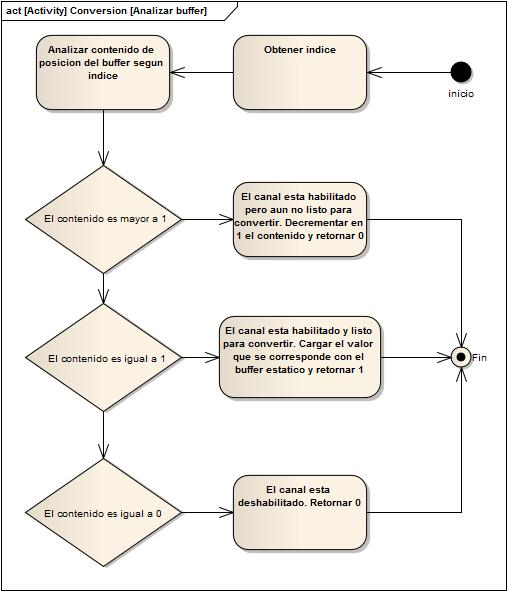
\includegraphics[width=0.80\textwidth, height = 7cm]{actividadanalizarbuffer}
  \caption[Diagrama de actividad de la funcion analizar buffer]{Diagrama de actividad que muestra el funcionamiento de la funcion analizar buffer. Esta funcion esta pensada para trabajar junto con "cambiar\_pin". En cada cambio de pin, se analiza el buffer para saber si hay que convertir o no, y actualizar el estado de los elementos del buffer, que corresponden en uno a uno con todas las vias de conversion posibles.}\label{fig:actividadanalizarbuffer}
\end{figure}



\begin{figure}[h]
  \centering
  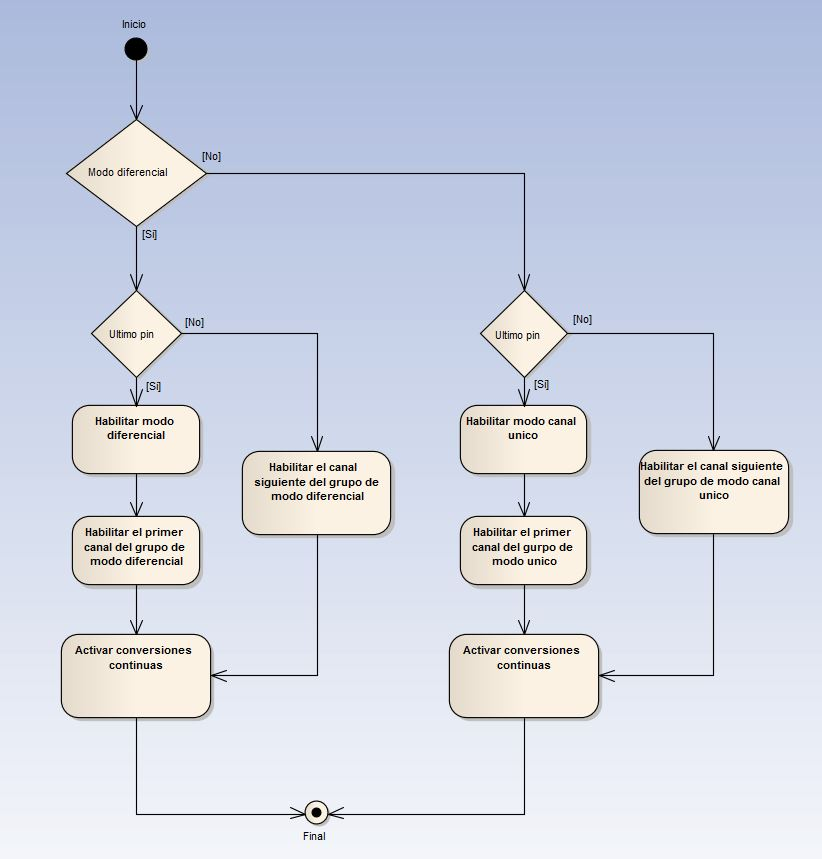
\includegraphics[width=0.80\textwidth, height = 7cm]{actividadcambiarpin}
  \caption[Diagrama de actividad de la funcion cambiar pin]{Diagrama de actividad que ilustra la logica dentro de la funcion cambiar\_pin, dentro del modulo del conversor. Esta funcion es llamada luego de cada conversion. En cada llamado, se selecciona un nuevo canal a medir. No discrimina si el canal esta o no habilitado para medir, en caso en que no lo este, se llamara inmediatamente para cambiar el pin nuevamente sin realizar medicion alguna.}\label{fig:actividadcambiarpin}
\end{figure}

\subsubsection{Marca de tiempo} % (fold)
\label{ssub:marca_de_tiempo}

En algunos casos, puede ser necesario saber la hora, minuto y segundo en el que se midió. Para esto, sugerimos la idea de que se incluya una marca de tiempo dentro de los meta-datos enviados a la placa de gestion. Fue un requerimiento propuesto por nosotros en una etapa ya avanzada del proyecto. Esta marca de tiempo es necesariamente relativa al momento de inicio de conversiones continuas. Esto se debe a que la placa de instrumentacion no tiene manera directa de calcular la fecha y hora exacta del dia, por lo que obtener una marca de tiempo absoluta de manera directa en esta placa no es practico. 
La solucion planteada para obtener una marca de tiempo absoluta fue calculandola en la placa de gestion. Al estar esta placa conectada a internet, puede obtener facilmente la fecha y hora de inicio de conversiones. Con esto, a la fecha y hora se le suma la marca relativa de cada medicion, y se obtiene asi la marca de tiempo absoluta. Sabiendo esto, en esta seccion explicamos la obtencion de la marca de tiempo relativa. La absoluta se describe en la seccion \ref{it6:ssub:obtencion_de_marca_de_tiempo_absoluta}. \\

El proceso para obtener la marca de tiempo esta descripto en la imagen \ref{fig:secuenciaobtenermarca} mediante un diagrama de secuencia. La marca de tiempo relativa se obtiene con el uso del timer2. Esto significa reducir la cantidad de contadores de eventos disponibles de 2 a 1, lo cual afecta de manera directa a un requerimiento principal. La solucion planteada fue dejar como opcional el calculo del timestamp, pudiendo asi elegir el uso del timer2 entre contador de eventos o contador interno para la marca de tiempo. Esto es posible porque hay casos donde no es necesario ser preciso a la hora de tener el tiempo de las mediciones, y se pueden calcular las marcas directamente desde el sistema de gestion, y asi dejar libre al timer2 para el conteo de eventos. Esto fue un compromiso dado el estado avanzado del proyecto.


\begin{figure}[h]
  \centering
  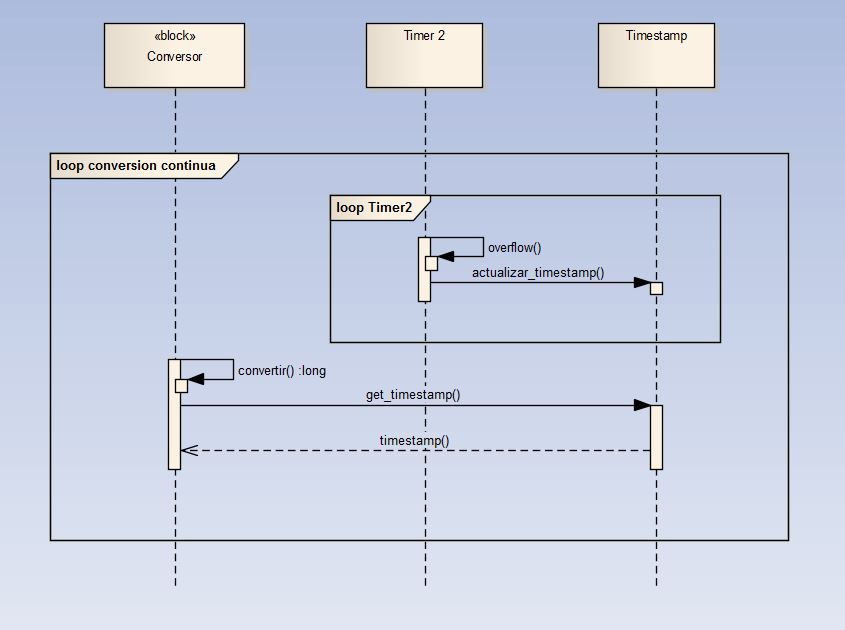
\includegraphics[width=0.80\textwidth, height = 7cm]{secuenciaobtenermarca}
  \caption[Diagrama de secuencia para la obtencion de una marca de tiempo]{Diagrama de secuencia que muestra la interaccion entre el conversor y timer 2 para obtener la marca de tiempo. En el diagrama, la marca de tiempo esta representada mediante un objeto que alberga un unico campo, que es la marca de tiempo. En cada interrupcion de Timer 2 este valor se actualiza, y en cada conversion se obtiene el valor actual para enviarlo junto con la medicion obtenida en la conversion.}\label{fig:secuenciaobtenermarca}
\end{figure}

% subsubsection marca_de_tiempo (end)

% subsection conversor (end)

\subsection{Interfaz de usuario} % (fold)
\label{it5:sub:interfaz_de_usuario}

La interfaz de usuario siguio un diseño parecido al terminado en la iteracion \ref{iteracion_2}. Gracias al diseño de la interfaz, agregar nuevos comandos con nuevos argumentos era facil siempre y cuando se respetara la expresion regular.

Los comandos disponibles al final de esta iteracion fueron:

\begin{itemize}
  \item SSE: - \textit{set single ended}: Establece un canal en modo unico.
  \item SDI: - \textit{set differential}: Establece un par de canales en modo diferencial.
  \item GSE: - \textit{get single ended}: Obtiene una conversion instantanea en modo canal unico sobre un canal.
  \item GDI: - \textit{get differential}: Obtiene una conversion instantanea en modo diferencial sobre un par de canales.
  \item GDI: - \textit{get differential}: Obtiene una conversion instantanea en modo diferencial sobre un par de canales.
  \item SGA: - \textit{set gain}: Establece el nivel de ganancia del conversor.
  \item GT0: - \textit{get timer 0}: Obtiene el valor actual de la cuenta de timer 0, configurado como contador de eventos.
  \item GT2: - \textit{get timer 2}: Obtiene el valor actual de la cuenta de timer 2, configurado como contador de eventos.
  \item SHA: - \textit{show configuration}: Muestra la configuracion actual de todos los canales y la ganancia del conversor.
  \item ST: - \textit{start}: Inicia el modo de conversiones continuas.
\end{itemize}

El conjunto entero de comandos esta documentado con mayor detalle en el apendice \ref{ap:instrucciones}.
% subsection interfaz_de_usuario (end)

\subsection{Memoria flash} % (fold)
\label{it5:sub:memoria_flash}

La memoria flash del microcontrolador puede ser utilizada para guardar las configuraciones actuales, de forma que si el sistema se apaga, se pueda volver a iniciar con las configuraciones ya cargadas, sin necesidad de volver a establecer todo cada vez que se inicie nuevamente. Esto fue planteado como requerimiento para esta iteracion, pero no pudo ser posible. Las operaciones necesarias para leer y escribir la memoria y el tamaño de la misma hicieron que sea difícil realizar la escritura y la lectura de la misma.

Tanto el programa que corre en el microprocesador como los datos de configuración debe guardarse en la misma memoria flash de 8Kb, siendo que el programa ocupa alrededor de 7Kb. En el Kb que resta, es posible guardar las configuraciones, pero el método de escritura de la flash pone en riesgo la integridad del programa. La unica manera de escribir en memoria es haciendolo sobre una pagina de 512 bytes. Dado el reducido espacio disponible, era probable que en una escritura se sobreescribiera parte del programa, haciendo que el sistema falle.
Teniendo en cuenta esto, se decidió no utilizar la flash para guardar las configuraciones. Por lo tanto, cada vez que el sistema se apague, se pierden las configuraciones, sin posibilidad de guardarlas.

% subsection memoria_flash (end)

% section desarrollo (end)

\section{Pruebas} % (fold)
\label{it5:sec:pruebas}

\begin{table}[h]
\centering
\caption{Test de sistema 1}
\label{it5:tab:testsistema1}
\begin{tabular}{p{2cm} p{9cm}}
\multicolumn{2}{c}{\cellcolor[HTML]{68CBD0}{\color[HTML]{000000} Prueba de sistema}} \\
Prueba \#        & 3 \\
\hline
Nombre           & Comportamiento esperado del conversor \\
\hline
Requerimiento & Se deberian poder configurar tiempos de intervalo entre cada medicion para cada canal por separado. \\
\hline
Descripcion      & Con este test, se comprueba que el sistema permite establecer intervalos de medicion individuales para cada canal, y que se comporta de manera consistente con el el paso del tiempo. \\
\hline
Pre-condiciones  & \tabitem Sistema configurado con dos pines en modo canal unico \\
                 & \tabitem Un canal esta configurado con un tiempo de 1 y otro con 50 \\
                 & \tabitem Generadores de tension conectados a los pines configurados  \\
                 & \tabitem Computadora conectada al sistema mediante cable serial RS-232 \\
                 & \tabitem Lector de canal serial abierto en la computadora  \\
                 & \tabitem Sistema midiendo en modo de conversiones continuas\\
\hline

Post-condiciones & La frecuencia de medicion para el canal en 1 deberia ser mayor a la frecuencia del canal en 50.                     
\\
\hline
Secuencia  & \tabitem Establecimos una tension de 1,5 voltios en el primer generador, conectado al canal con intervalo 1 y una de 2 voltios en el segundo, con intervalo 50 \\
\hline
Resultados       & El canal con intervalo 1 tenia una frecuencia mucho mayor al canal con intervalo 50, que era lo esperado. La relacion entre las frecuencias parecia ser lineal (50 veces mas frecuente el primero que el segundo), aunque no teniamos una manera precisa de medirlo, mas que contar la cantidad de mediciones en un intervalo grande de tiempo.
\end{tabular}
\end{table}

\begin{table}[h]
\centering
\caption{Test de sistema 2}
\label{it5:tab:testsistema2}
\begin{tabular}{p{2cm} p{9cm}}
\multicolumn{2}{c}{\cellcolor[HTML]{68CBD0}{\color[HTML]{000000} Prueba de sistema}} \\
Prueba \#        & 3 \\
\hline
Nombre           & Generacion de la marca de tiempo \\                 
\hline
Requerimiento & Se deberia generar una marca de tiempo relativa al inicio de conversiones en cada medicion realizada. \\
\hline
Descripcion      & En cada conversion, se deberia registrar una marca de tiempo con un numero que hace referencia al tiempo que transcurrio desde el momento que se iniciaron las conversiones al momento donde se toma la medicion. \\
\hline
Pre-condiciones  & \tabitem Sistema configurado con un pin en modo canal unico, con un intervalo de 10, que corresponde a SEGUNDOS segundos segun la tabla LA TABLAAA \\
                 & \tabitem Generador de tension conectado al pin configurado  \\
                 & \tabitem Computadora conectada al sistema mediante cable serial RS-232 \\
                 & \tabitem Lector de canal serial abierto en la computadora  \\
                 & \tabitem Cronometro en 00:00\\
                 & \tabitem Reloj en hora\\
\hline

Post-condiciones & La diferencia entre cada marca de tiempo y la siguiente deberia ser constante, y deberia ser aproximada al valor en segundos dado por el intervalo. El calculo en fecha y hora de la ultima marca de tiempo y el valor del cronometro (hecho con ayuda del reloj) deberia dar aproximadamente igual. VER ESTO ACA PORQUE HAY UN DRAMA CON EL TEMA PRECISION QUE NO LO DISCUTIMOS MUCHO Y HABRIA QUE DEFINIRLO \\
\hline
Secuencia  & \tabitem Establecimos una tension en el generador.
           & \tabitem En simultaneo, dimos arranque al cronometro y iniciamos las conversiones continuas.
           & \tabitem Luego de 10 segundos, paramos el cronometro y las conversiones, tambien en simultaneo.

Resultados       & VA A HABER QUE HACERLO
\end{tabular}
\end{table}

\begin{table}[h]
\centering
\caption{Test de sistema 3}
\label{it5:tab:testsistema3}
\begin{tabular}{p{2cm} p{9cm}}
\multicolumn{2}{c}{\cellcolor[HTML]{68CBD0}{\color[HTML]{000000} Prueba de sistema}} \\
Prueba \#        & 3 \\
\hline
Nombre           & Formato esperado del mensaje \\                     
\hline
Requerimiento    & \tabitem Los datos que se envian a la placa de gestion para cada medicion deberia inculir, ademas de la medicion, el numero de pin o pines (si es mododiferencial) de donde se esta midiendo.  \\
                 & \tabitem Los datos que se envian a la placa de gestion para cada medicion deberia inculir, ademas de la medicion, el modo de conversion del canal por donde se esta midiendo.
                 & \tabitem Los datos que se envian a la placa de gestion para cada medicion deberia inculir, ademas de la medicion, la marca de tiempo relativa correspondiente de la medicion hecha. 
\hline
Descripcion      & Cada dato que se envia a la placa de gestion incluye la siguiente informacion: Medicion, pin, modo, marca de tiempo. Estos datos estan enviados con un formato especial, y se envian en simultaneo. Esta prueba verifica que cada mensaje contenga el formato correcto y que los datos sean coherentes a las configuraciones. \\
\hline
Pre-condiciones  & \tabitem Sistema configurado con el pin 3 en modo canal unico, con un intervalo de 10 \\
                 & \tabitem Generador de tension conectado al pin configurado con un valor de 1,5 volts  \\
                 & \tabitem Computadora conectada al sistema mediante cable serial RS-232 \\
                 & \tabitem Lector de canal serial abierto en la computadora  \\
                 & \tabitem Sistema midiendo en modo de conversiones continuas\\
\hline

Post-condiciones & El mensaje recibido en el lector serial deberia ser "1500,3,SE,[marca de tiempo]".                     
\\
\hline
Resultados       & El formato era correcto
\end{tabular}
\end{table}

% section pruebas (end)

\section{Conclusiones} % (fold)
\label{sec:conclusiones}

En esta iteracion, llegamos a obtener un prototipo final del software, listo para embeber en el microcontrolador dentro de la placa construida en las iteraciones anteriores. No se cubrieron todos los requerimientos, pero si los de mayor riesgo:

\begin{itemize}
\item Es posible configurar tiempos de intervalo entre cada medicion para cada canal por separado
\item Los datos que se envian a la placa de gestion para cada medicion incluyen, ademas de la medicion, el numero de pin o pines (si es modo diferencial) de donde se esta midiendo. 
\item Los datos que se envian a la placa de gestion para cada medicion incluyen, ademas de la medicion, el modo de conversion del canal por donde se esta midiendo.
\item Los datos que se envian a la placa de gestion para cada medicion incluyen, ademas de la medicion, la marca de tiempo relativa correspondiente de la medicion hecha. 
\end{itemize}

Las funciones correspondientes al conversor, son las que hacen de mayor utilidad a la placa, yendo mas alla de las funcionalidades que el microcontrolador ya posee de manera nativa. Esto es, entre otras cosas, la posibilidad de configurar cada canal por separado, en el modo que se desee, y con un intervalo de tiempo que cubre una ventana amplia.

El uso de la marca de tiempo fue implementado, pero con la particularidad de que utiliza uno de los contadores del microcontrolador, restando en 1 la cantidad de contadores de eventos disponibles. Optamos por dejarlo como opcion al usuario de usar la marca de tiempo o usar el contador.


% section conclusiones (end)

% chapter iteracion_5 (end)

\chapter{Iteracion 6: Implementacion de un sistema gestionador para la placa de instrumentacion} % (fold)
\label{cha:iteracion_6}

\section{Introduccion} % (fold)
\label{sec:introduccion}

El sistema de instrumentacion recibe, interpreta y distribuye datos de sensores, para luego enviarselas a otro sistema que extiende las funciones del primero, teniendo entonces un sistema de gestion y administracion para los datos de los sensores. En esta iteracion, realizamos una implementacion de este ultimo sistema. La idea es tener un sistema cuyas funciones incluyan el manejo de la placa de instrumentacion, pero que ademas, permita un uso mas general en lo que respecta al manejo de sistemas administradores de sensores y actuadores
La figura \ref{fig:topologiaplacas} muestra una topologia basica que describe el rol de este sistema a implementar.

% section introduccion (end)

\section{Requerimientos de la iteracion} % (fold)
\label{sec:requerimientos_de_la_iteracion}

\begin{itemize}
\item El sistema deberia estar implementado en una placa de desarrollo de manera que se pueda conectar a la placa de instrumentacion via comunicacion serial
\item Deberia estar en el mismo lugar fisico que la placa de alimentacion.
\item Deberia implementar un servidor web con una interfaz grafica de usuario. Esta interfaz deberia permitir:
\begin{itemize}
	\item Las mismas acciones que si el usuario se conectara directamente con la placa de instrumentacion via interfaz de comando, solamente que via interfaz grafica.
	\item Enviar cualquier comando que pueda ser interpretado por la placa de instrumentacion
	\item Establecer intervalos de tiempo usando hora y fecha en los que se debe medir sobre cierto canal
\end{itemize}
\item Deberia guardar datos de mediciones e informacion sobre transacciones en general entre ambas placas en una base de datos local, accesible via la interfaz grafica 
\item La conexion entre el sistema y el usuario (dispositivo del usuario) deberia ser via Wi-Fi o algun otro protocolo inalambrico
\end{itemize}


% section requerimientos_de_la_iteracion (end)

\section{Desarrollo} % (fold)
\label{sec:desarrollo}

\subsection{Placa de desarrollo elegida para la implementacion} % (fold)
\label{sub:placa_de_desarrollo_elegida_para_la_implementacion}

Sin una seleccion previa teniendo en cuenta los requisitos, y por una cuestion de accesibilidad, se decidio implementar este sistema en una placa de desarrollo Raspberry Pi B+ (figura \ref{fig:raspberrypi}), embebida con un sistema operativo Raspbian (Debian para Raspberry). Bajo estas condiciones, es posible cubrir todos los requerimientos.

\begin{figure}[h]
  \centering
  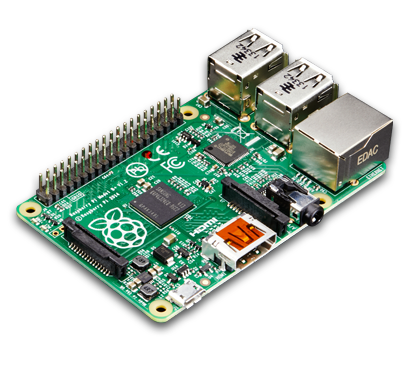
\includegraphics[width=0.80\textwidth, height = 7cm]{raspberrypi}
  \caption{Placa de desarrollo Raspberry Pi B+}\label{fig:raspberrypi}
\end{figure}
% subsection placa_de_desarrollo_elegida_para_la_implementacion (end)

\subsection{Servidor web} % (fold)
\label{sub:servidor_web}

% subsection servidor_web (end)

\subsection{Base de datos} % (fold)
\label{sub:base_de_datos}

% subsection base_de_datos (end)

\subsection{Interfaz grafica de usuario} % (fold)
\label{sub:interfaz_grafica_de_usuario}

% subsection interfaz_grafica_de_usuario (end)

% section desarrollo (end)

\section{Pruebas} % (fold)
\label{sec:pruebas}

% section pruebas (end)

\section{Resultados} % (fold)
\label{sec:resultados}

% section resultados (end)

% chapter iteracion_6 (end)

\chapter{Iteracion 7: Caso de prueba con un sensor de campo electrostatico} % (fold)
\label{cha:iteracion_7}

\section{Introduccion} % (fold)
\label{sec:introduccion}

Parte de este proyecto fue poner a prueba nuestro sistema utilizando un sensor detector de campo electrostatico. Ademas de obtener las mediciones, fue necesario realizar un sistema de control para el motor del sensor. En esta iteracion realizamos la adaptacion necesaria de los requisitos de funcionamiento del sensor a nuestro sistema de instrumentacion, probando asi el funcionamiento del mismo, asi como tambien el funcionamiento del sistema gestionador desarrollado en la iteracion \ref{cha:iteracion_6} 

\subsection{Marco teorico} % (fold)
\label{sub:marco_teorico}

La intensidad de un campo electrico se puede medir, en principio, colcando un medidor de voltaje entre dos placas metalicas paralelas separadas por una distancia. El problema de esto es que, como el medidor de voltaje suele tener una impedancia alta en la entrada, cualquier voltaje inducido en las placas se pierde rapidamente, y no podria usarse para medir el capo electrico. Para arreglar esto, se utiliza la tecnica de las aspas. Se coloca una placa conductora, y sobre la misma se posiciona un sistema con aspas de forma que cuando estas roten, se cubra y se exponga periodicamente la placa conductora al campo electrico ambiental. Para lograr esto apropiadamente, el rotor que hace girar las aspas debe estar conectado a tierra. La placa conductora esta conectada a tierra a traves de un amplificador de transconductancia, que convierte la corriente que va desde la placa a tierra en una tension.
A medida que la placa conductora este expuesta al campo electrico, el campo induce una corriente a tierra mientras que atrae o repele la carga de la placa conductora. A medida que la placa esta cubierta del campo electrico, la carga inducida se drena. Entonces las placas inducen una corriente alterna a masa que es proporcional a la intensidad del campo electrico estatico. Esta corriente alterna luego puede ser rectificada para utilizarla como entrada a un conversor analogico digital y obtener asi la intensidad del campo electrico medido. \\

Una vez obtenida la intensidad, es necesario saber el signo del campo electrico medido. Para obtenerlo, un metodo es que en el mismo conversor analogico digital se obtenga la medicion de manera diferencial. Un conversor analogico digital diferencial toma la diferencia entre dos canales para obtener un dato en lugar de tomar el valor de un canal y compararlo con tierra. De forma que es posible determinar cual es el canal con mayor tension. Con esto, se pueden conectar los canales de las señales de tierra y la de la placa conductora, y se miden de manera diferencial para obtener tento la intensidad como el signo del campo electrico estatico.
\cite{sensorcampo}

% subsection marco_teorico (end)
\subsection{El sensor} % (fold)
\label{sub:el_sensor}

El sensor utilizado es un dispositivo que mide la intensidad del campo electrico en el ambiente debido al campo electrostatico generado por la carga electrica de las nubes en el momento. Se puede utilizar para detectar la posibilidad de que caiga un rayo en una zona cercana al sensor, y tambien para investigar los efectos de la electricidad estatica. Para funcionar, el sensor necesita de un motor que gire a velocidad constante. Este motor funciona en base a un driver que tiene como entrada una señal modulada por ancho de pulso.
Mientras el motor gire a velocidad constante, es posible obtener datos validos del sensor. La idea es hacer que el funcionamiento del sensor como la adquisicion de las mediciones sea logrado con funcionalidades de la placa de instrumentacion, mas otras caracteristicas que ofrece el microcontrolador C8051F352, como ser el modulo de PWM para generar la señal modulada por ancho de pulso, y el uso de los timers para establecer las bases de tiempo que utilizamos para hacer un control de estabilidad en la velocidad del motor. \\

Fisicamente, es una estructura metalica compuesta por un motor que hace girar unas aspas que se se encargan de blindar y desblindar una placa que a su vez se carga y descarga con la electricidad estatica del ambiente. esta carga y descarga continua es lo que justamente se termina transformando en el nivel de voltaje que nos indica el nivel de electricidad estatica del ambiente, que es lo que queremos saber.
La placa y las aspas funcionan como un capacitor que se blinda y se des\-blinda a medida que el motor gira. En el momento que las aspas estan descuburiendo la placa, el capacitor se carga, y en el momento que se cubre la placa, el capacitor se descarga. La descarga se hace sobre un amplificador que luego va a un conversor analogico digital, que termina en la lectura de un valor que nos dice el nivel del campo electrostatico ambiental. En el caso particular de este sensor, el motor que hace girar las aspas es un motor brushless manejado por un driver PWM.

\begin{figure}[h]
  \centering
  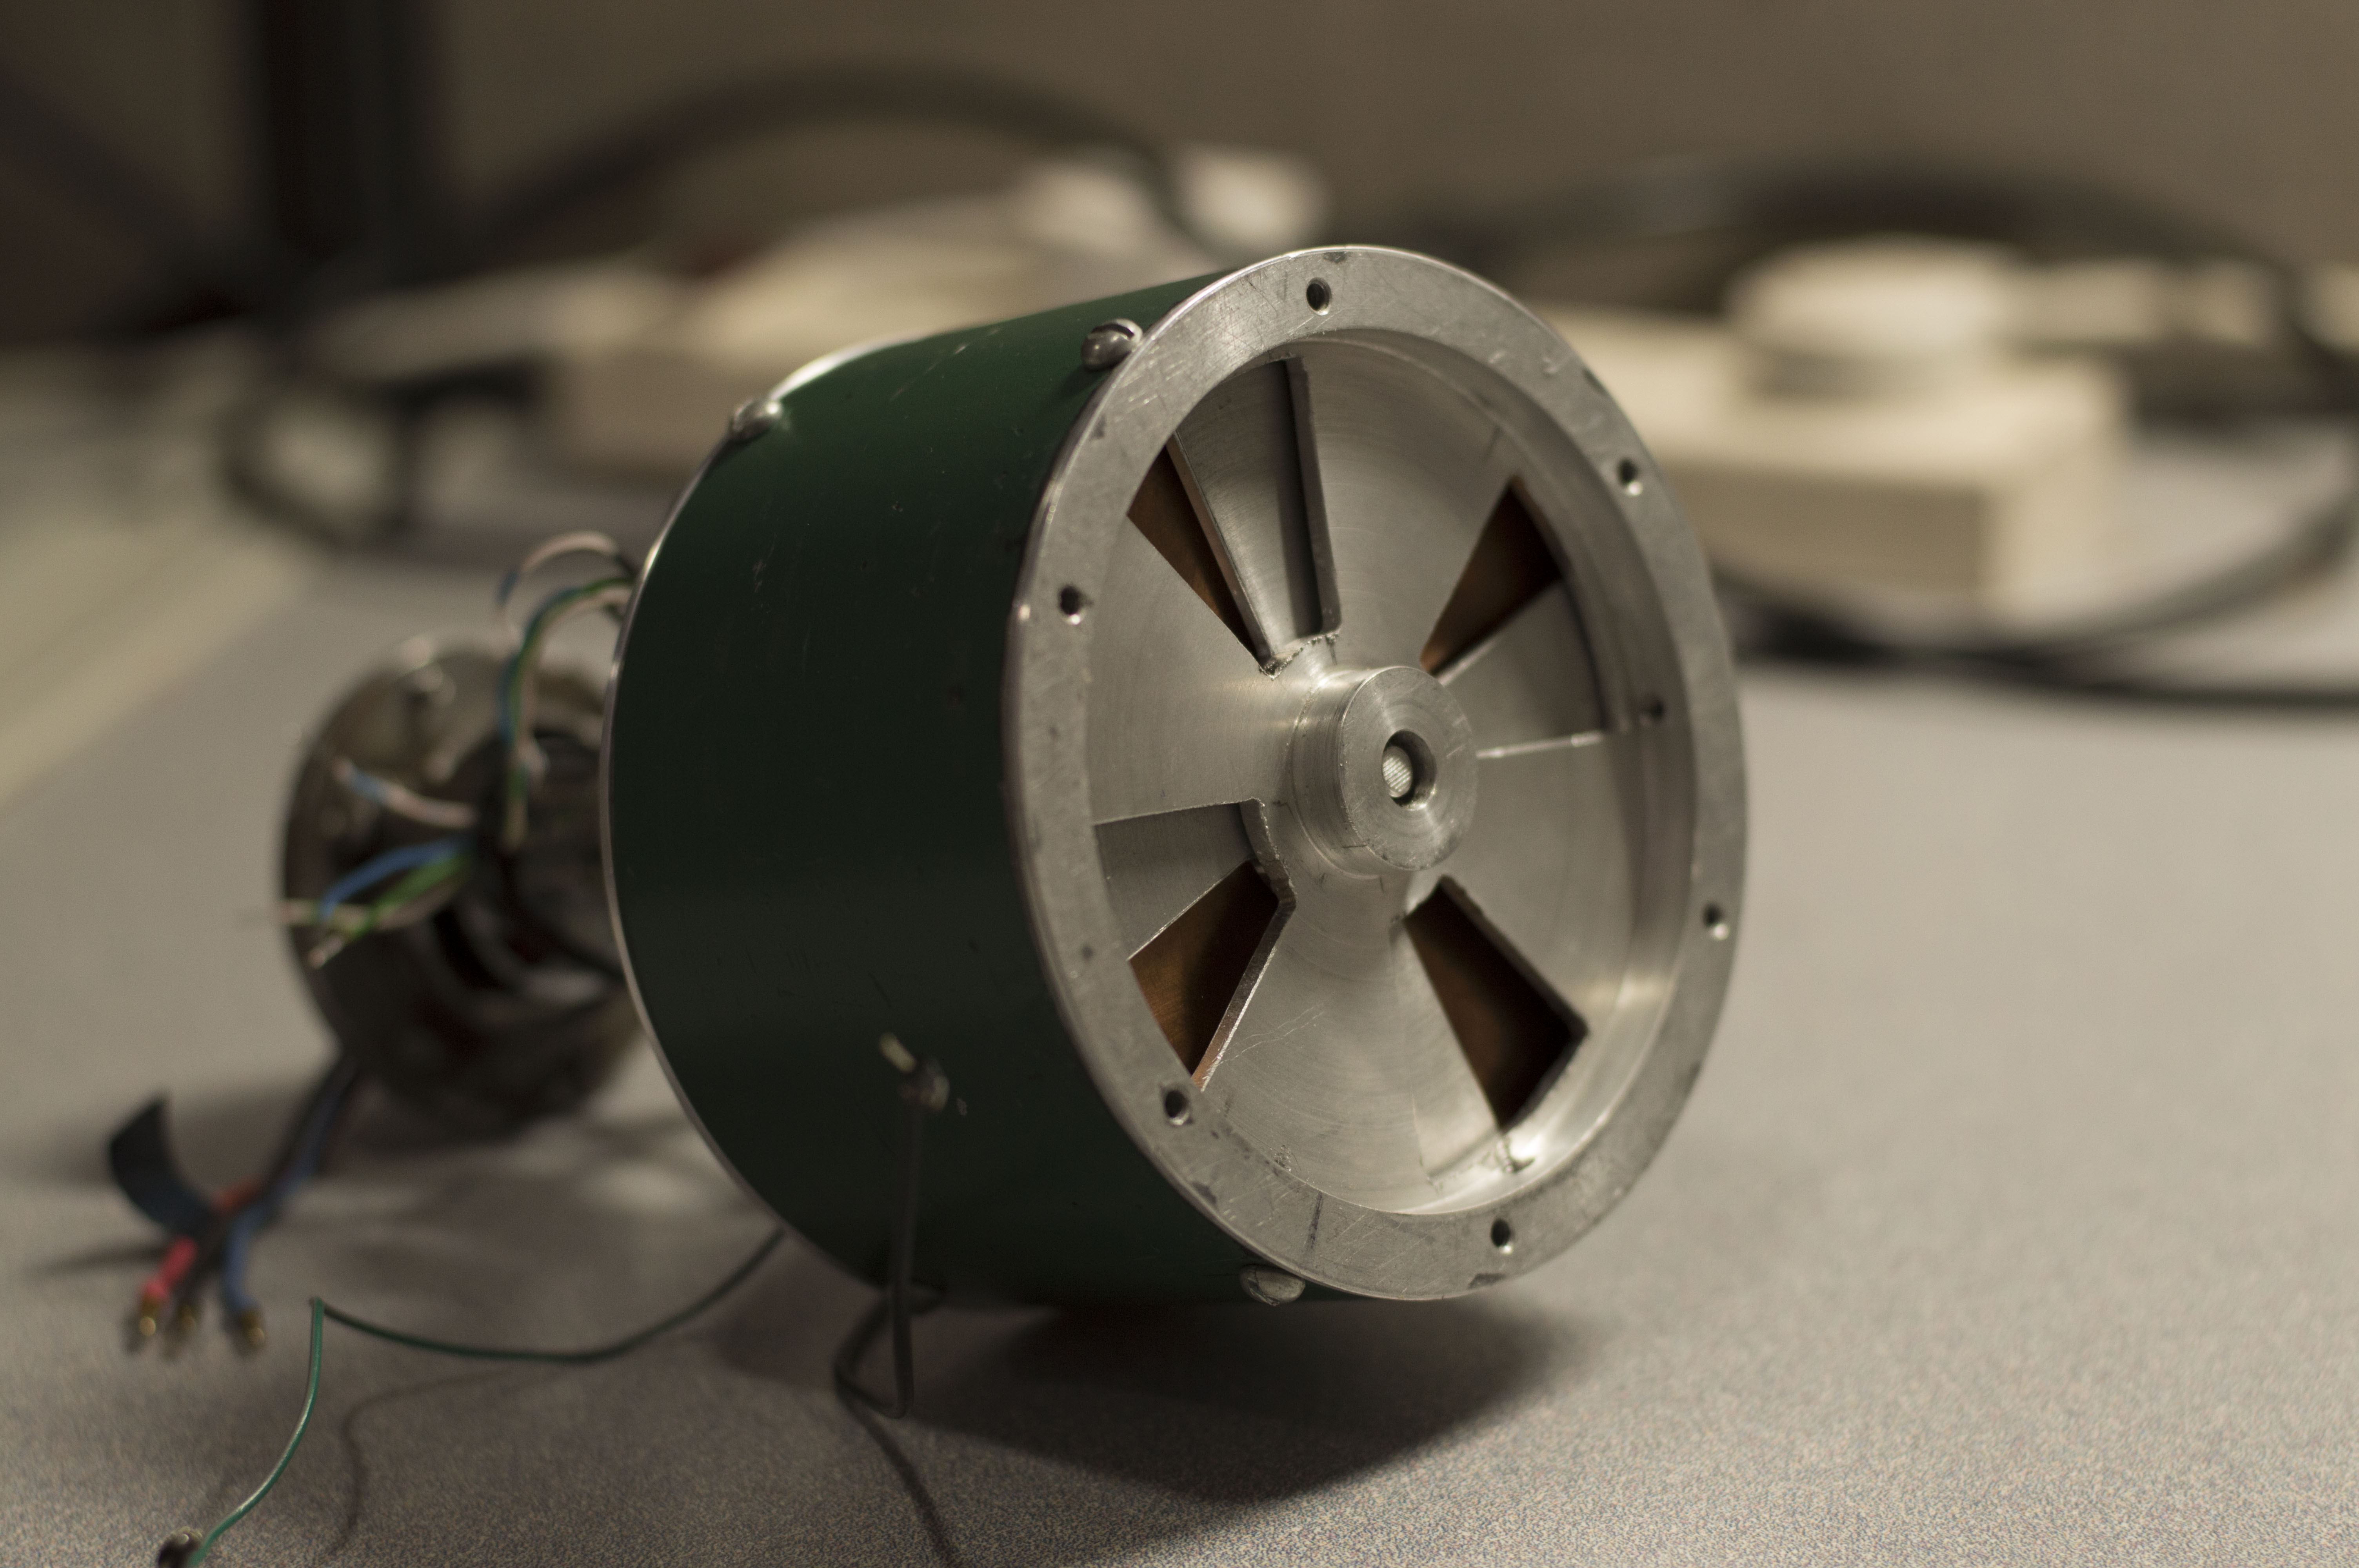
\includegraphics[width=0.80\textwidth, height = 7cm]{sensorhorizontal}
  \caption[Imagen del sensor de campo electrostatico utilizado (horizontal)]{Foto del sensor en horizontal. Las aspas que pueden verse son las responsables de cubrir y descubrir la placa cargada (color cobre), que es la que se carga con la electricidad estatica del ambiente.}\label{fig:sensorhorizontal}
\end{figure}

\begin{figure}[h]
  \centering
  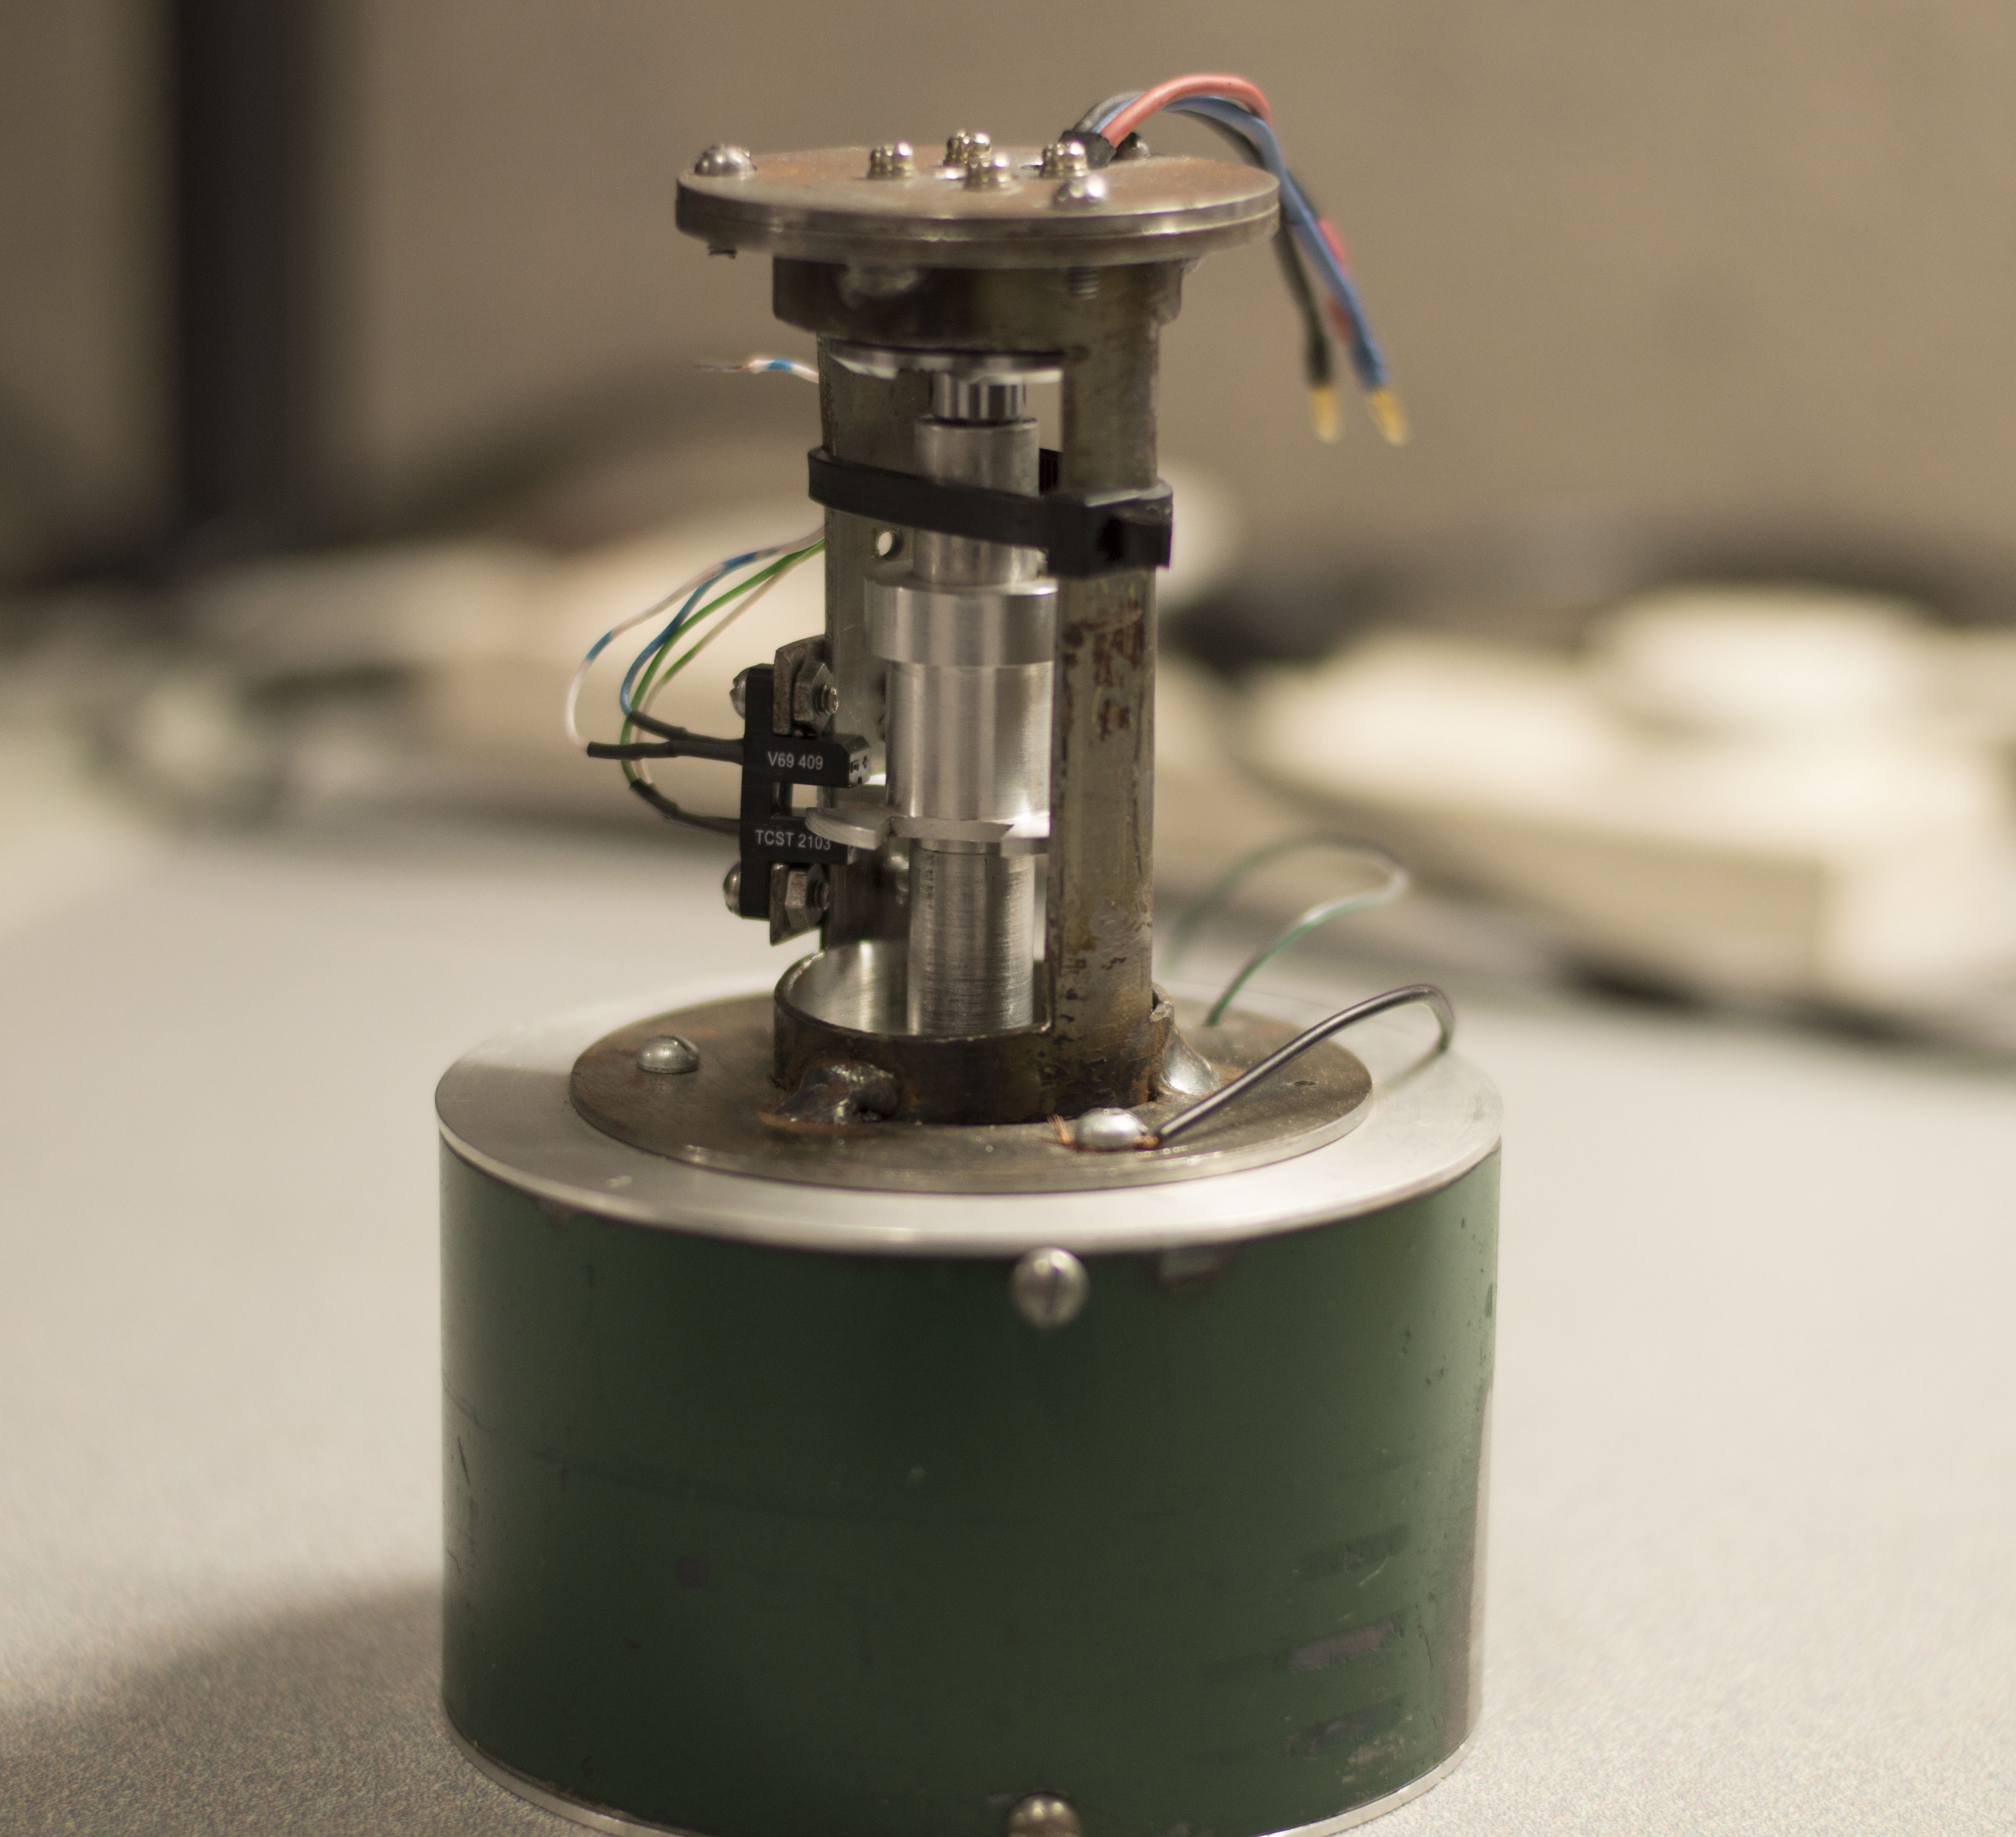
\includegraphics[width=0.80\textwidth, height = 7cm]{sensorvertical}
  \caption[Imagen del sensor de campo electrostatico utilizado (vertical)]{Foto del sensor en vertical. Puede verse en el eje, el sistema de aspas y fotointerruptor utilizado para medir las RPM.}\label{fig:sensorvertical}
\end{figure}

Ademas de las aspas que miden el campo electrico, en el eje del motor se encuentra un segundo grupo de aspas, pero mas pequeño; junto a estas aspas se encuentra acoplado un fotointerruptor, de manera que el paso de cada aspa interrumpe el paso de luz de un extremo a otro. Si se construye el circuito requerido para el fotointerruptor, ocurrira que cuando el motor este girando, se generen pulsos cuadrados a la salida del fotointerruptor, permitiendo obtener cuentas que ayudaran a la hora de controlar la velocidad del motor. Las aspas secundarias y el fotointerruptor pueden verse en la figura \ref{fig:sensorvertical}

% subsection el_sensor (end)

% section introduccion (end)

\section{Requerimientos de la iteracion} % (fold)
\label{sec:requerimientos_de_la_iteracion}

\begin{itemize}
\item Se deberian utilizar las funcionalidades de los sistemas desarrollados en el transcurso del proyecto para obtener mediciones del sensor
\item Se deberia controlar la velocidad del motor utilizando el fotointerruptor
\item Se deberia diseñar y construir una placa con un circuito de adaptacion para el funcionamiento y la operacion del sensor
\item La placa de adaptacion deberia poder ser acoplable a la placa de instrumentacion (como shield)
\item Se deberia construir un recipiente donde pueda entrar el sensor junto con el sistema de instrumentacion y el sistema gestionador, para poder colocarlo en el aire libre con el objetivo de realizar una prueba de campo
\end{itemize}


% section requerimientos_de_la_iteracion (end)

\section{Experimentacion} % (fold)
\label{sec:experimentacion}

El motor dentro de este sensor incluia un driver PWM. Para arrancar y dar velocidad a este motor, se utilizo, como primera instancia, una placa de desarrollo Arduino con un software hecho por Emiliano Pellicioni y Diego Gutierrez. Con el driver conectado a la placa y el programa funcionando, era posible arrancar el motor y darle una velocidad (aunque no muy constante).

Teniendo el motor funcionando, la teoria indica que el sensor esta midiendo campo. Para probar esto, se utilizo una regla de plastico cargada con electricidad estatica y un osciloscopio conectado a la salida del sensor. Al acercar y alejar la regla de las aspas, se podia ver en la salida del osciloscopio como la onda resultante a la salida del sensor aumentaba y disminuia en amplitud. Lo que estabamos viendo, en ese momento, era una salida ``en crudo'' del sensor. Para poder convertir la señal y obtener datos coherentes, era necesario rectificar la señal. \\

El fotointerruptor acoplado al eje del motor da la posibilidad de realizar un conteo de señales cuadradas que nos proporcione los datos suficientes como para realizar una medicion de las vueltas por minuto del motor. Necesita de un circuito basico para funcionar. Lo construimos en una protoboard junto con todo lo necesario para hacer funcionar el motor. Con ayuda de un osciloscopio, fue posible ver los pulsos cudadrados de 5 Volts generados por el fotointerruptor. Estos pulsos son los que luego servirian de entrada a un contador de eventos de la placa de instrumentacion, con el objetivo de controlar la velocidad del motor. \\

ACA FALTARIA INCLUIR IMAGENES DE:

-EL OSCILOSCOPIO CON LA SALIDA DEL SENSOR MIDIENDO
-EL OSCILOSCOPIO CON LA SALIDA DEL FOTO INTERRUPTOR

% section experimentacion (end)

\section{Implementacion de una placa de adaptacion para el sensor de campo} % (fold)
\label{sec:implementacion_de_una_placa_de_adaptacion_para_el_sensor_de_campo}

Para el debido funcionamiento y control del sensor, se planteo en los requerimientos el desarrollo de una placa con que contenga los circuitos necesarios para alimentar el motor, tratar la señal de medicion de campo, y tratar los pulsos cuadrados del fotointerruptor, de forma que la placa de instrumentacion pueda leer ya procesados los datos necesarios para medir el campo y controlar la velocidad del motor.


\subsection{Requerimientos} % (fold)
\label{sub:requerimientos}

A partir de estas pruebas sacamos las siguientes conclusiones para el circuito de adaptacion del sensor:

\begin{itemize}
	\item Debe poder conectarse la alimentacion y las entradas PWM del driver del motor
	\item Debe incluir un circuito de adaptacion (rectificacion y amplificacion) de la señal del sensor
	\item Debe incluir el circuito necesario para el funcionamiento del fotosensor.
	\item El diseño de la placa deberia ser tal que sea acoplable y desacoplable a la placa de instrumentacion.
\end{itemize}

Mediante investigacion y prueba y error, se desarrollaron los circuitos necesarios para cumplir con estos requerimientos y se fusionaron en un unico circuito que luego iria impreso en una placa. Para mejorar la practicidad, la placa deberia poder ser acoplable y desacoplable a la placa de instrumentacion. Esto ultimo se tuvo en cuenta a la hora de diseñar el despliegue de componentes y las dimensiones de la placa.

% subsection requerimientos (end)
\subsection{Circuito de adaptacion para la señal de nivel de campo} % (fold)
\label{sub:circuito_de_adaptacion_para_la_señal_de_nivel_de_campo}

aca va el operacional con el amplificador y rectificador que se pone para que vaya antes del conversor.. con imagen

% subsection circuito_de_adaptacion_para_la_señal_de_nivel_de_campo (end)

\subsection{Circuito de adaptacion para la señal de pulsos del fotointerruptor} % (fold)
\label{sub:circuito_de_adaptacion_para_la_señal_de_pulsos_del_fotointerruptor}

La figura \ref{fig:fotointerruptorcircuitotipico} muestra el circuito que implementamos para el fotointerruptor. Es un diseño tipico utilizado en la mayoria de los casos en los que se utiliza este tipo de sensor. 

\begin{figure}[h]
  \centering
  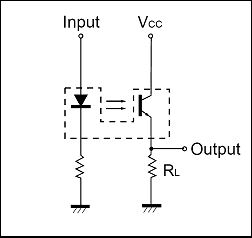
\includegraphics[width=0.80\textwidth, height = 7cm]{fotointerruptorcircuitotipico}
  \caption{Circuito utilizado para el fotointerruptor}\label{fig:fotointerruptorcircuitotipico}
\end{figure}

En esta disposicion, cuando el fotosensor esta iluminado, hay 5 Volts en la salida; de lo contrario 0 Volts. Esto hace que cuando el motor gira, las aspas van a tapar y destapar la entrada de luz al fotosensor generando una onda cuadrada a la salida del circuito, cuya frecuencia depende de la velocidad del motor.
Esta señal se utiliza como entrada para el contador de eventos, luego en el programa se calcula la velocidad del motor utilizando las cuentas obtenidas sobre una base de tiempo. 

% subsection circuito_de_adaptacion_para_la_señal_de_pulsos_del_fotointerruptor (end)

\subsection{Circuito de alimentacion} % (fold)
\label{sub:circuito_de_alimentacion}

La placa de instrumentacion esta diseñada para estar siempre encendida. Al no consumir mucho, no trae problemas de consumo o temperatura. Pero habiendo hecho esta adaptacion, era necesario tener en cuenta el consumo del motor mientras esta encendido pero sin girar. Para ahorrar consumo, propusimos agregar un control de encendido y apagado del sensor, utilizando uno de los pines GPIO del microcontrolador. \\

La figura PONER FIGURA DEL CIRCUITO muestra el circuito que prepara la señal del microcontrolador que controla el encendido y apagado del motor. Utilizamos un relé, un optoacoplador, un transistor, un diodo y resistencias. El optoacoplador sirve para aislar opticamente el circuito logico del motor con el circuito de 12 V. El rele electromecanico conmuta la conductividad entre el motor y masa, de manera que en un estado del rele el motor esta prendido, y en el otro esta apagado. Utilizamos un transistor porque los 5V a la salida del optoacoplador no eran suficientes para la tension de switching del relé.

% subsection circuito_de_alimentacion (end)

\subsection{Señal modulada en ancho de pulso para el driver del motor} % (fold)
\label{sub:señal_modulada_en_ancho_de_pulso_para_el_driver_del_motor}

% aca en realidad no hicimos nada porque lo unico que hay es el cable de salida del pwm que viene de la placa y se conecta de pecho al driver.. pero bueno explicar eso.. y explicar tambnein que pasamos desde el arduino que hacia todo por interrupciones al pwm de la placa que lo hace todo por HW y funciona mucho mejor. aunque no explicar como funciona el programa porque eso va despues

El driver del motor funciona a base de señales moduladas en pulso. Los anchos de pulso funcionan como codigos que representan distintos modos para el driver. El manual del driver especifica los distintos anchos de pulso que lo configuran de distintas maneras. Para guiarse en el proceso de configuracion, el driver suena con distintos ``beeps'' de distintos tonos que indican distintas cosas.

En nuestro caso, necesitabamos arrancar el motor y hacerlo a andar a una unica velocidad. Lo cual es uno de los modos mas simples. De igual manera, era necesario una serie de señales sucesivas con distintos anchos de pulso para arrancar el motor. Estas señales las hicimos utilizando un modulo del microcontrolador denominado PCA.





% subsection circuito_de_adaptacion_para_la_señal_modulada_en_ancho_de_pulso_para_el_driver_del_motor (end)

\subsection{Circuito final} % (fold)
\label{sub:circuito_final}


% subsection circuito_final (end)

% section implementacion_de_una_placa_de_adaptacion_para_el_sensor_de_campo (end)


\section{Funcionalidades desarrolladas dentro del software de la placa de instrumentacion para trabajar junto con el sensor} % (fold)
\label{sec:funcionalidades_desarrolladas_dentro_del_software_de_la_placa_de_instrumentacion_para_trabajar_junto_con_el_sensor}

Al programa embebido en el microcontrolador, le agregamos funcionalidades especificas para trabajar con este sensor. Realizamos un modulo aparte llamado sensor, cuyas funciones estan desarrolladas especificamente para este sensor y no otro. Estas funciones incluyen:

\begin{itemize}
	\item Dar arranque y parada al motor
	\item Establecer una velocidad al motor
	\item Controlar la velocidad del motor.
\end{itemize}

La medicion en si de los datos del sensor no esta como funcion especifica del mismo porque ya se cubre con las funciones ya hechas en el modulo del conversor.

\begin{figure}[h]
  \centering
  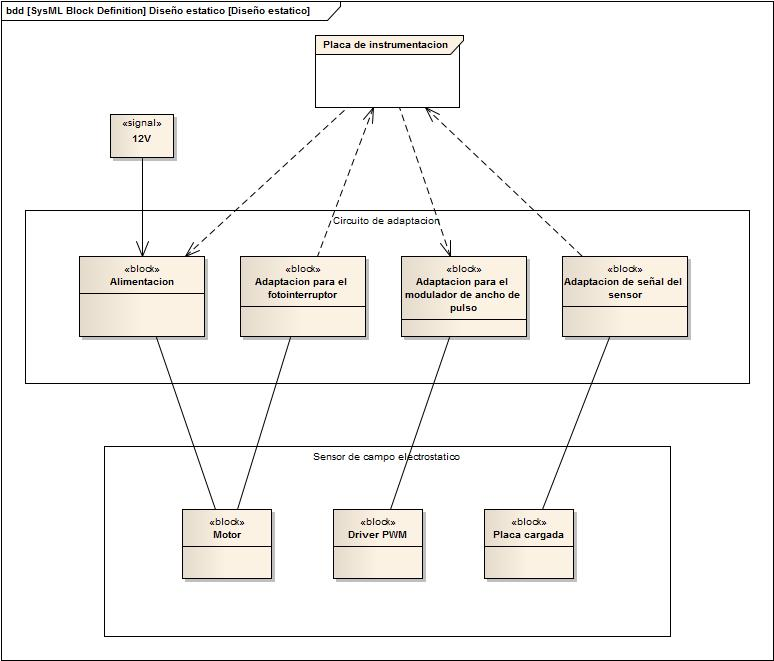
\includegraphics[width=0.80\textwidth, height = 7cm]{diagramabloquessensor}
  \caption{Diagrama de bloques fisicos del sistema de adaptacion del sensor}\label{fig:diagramabloquessensor}
\end{figure}

Y DE ACTIVIDAD PARA BER LA SUCESION DE COSAS QUE OCURREN CUANDO SE:
-PRENDE EL MOTOR
-SE CONTROLA VELOCIDAD

MAS QUE NADA.. ES LO MAS IMPORTANTE.

% section funcionalidades_desarrolladas_dentro_del_software_de_la_placa_de_instrumentacion_para_trabajar_junto_con_el_sensor (end)

\section{Pruebas} % (fold)
\label{sec:pruebas}

% section pruebas (end)

\section{Resultados} % (fold)
\label{sec:resultados}

% section resultados (end)

% chapter iteracion_7 (end)

\chapter{Conclusiones Finales} % (fold)
\label{cha:conclusiones}

\section{Sistema final} % (fold)
\label{sec:sistema_final}

El sistema obtenido es una \textbf{plataforma de instrumentación}, con dos microcontroladores C8051F352. Con 16 entradas analógicas, posibilitando 16 mediciones en canal único simultaneas, u 8 mediciones en modo diferencial simultaneas. Contiene, además 4 contadores de eventos de fuentes externas. Cada microcontrolador tiene un software embebido que permite configurar los distintos parámetros del sistema mediante una interfaz de linea de comando.

Como anexo a este sistema, obtuvimos un subsistema \textbf{controlador para un sensor de campo electrostático}. Tanto el software como el hardware fueron diseñados en este proyecto, y sirven para usar y controlar dicho sensor.

El \textbf{servidor web} implementado en la Raspberry Pi, es un caso de uso de un posible sistema embebido que trabaje junto con la plataforma. Este sistema esta especialmente diseñado para trabajar con la plataforma, específicamente con el uso del sensor de campo electrostático. Las funciones de la interfaz gráfica están orientadas al uso de este sensor. Sin embargo, permite cualquier tipo de configuración.

% section sistema_final (end)

\section{Trabajos Futuros} % (fold)
\label{sec:trabajos_futuros}

\begin{itemize}
	\item Utilizar otro microcontrolador para la plataforma, que permita el uso de una memoria flash para guardar configuraciones, y que permita utilizar $I^{2}$C.
	\item Acondicionar los aspectos electrónicos del sistema, mejorando su respuesta ante posibles inestabilidades de potencia
	\item Mejorar el circuito de adaptación para el sensor de campo electrostático en términos de reducción de consumo y ruido
	\item Extender el desarrollo del sistema que recibe los datos de la plataforma a un sistema de gestión de dispositivos IoT
	\item Refactorizar el diseño utilizando un patrón bien conocido
	\item Completar el desarrollo del detector inteligente de campo electrostático, utilizando la plataforma.
	\item Controlar ambos microcontroladores con un único software.
\end{itemize}

% section trabajos_futuros (end)


% chapter conclusiones (end)

\appendix
\appendix

\chapter{Instrucciones MML}\label{ap:instrucciones}
%%%%%%%%%%%%%%%%%%%%%%%%%%%%%%%%%%%%%%%%%%%%%%%%%%%%%%%%%%%%%%%%

\section{SSE: Set Single Ended} % (fold)
\label{sub:sse_set_single_ended}


\textbf{Formato:} SSE,[1],[1]

\textbf{Descripción:}
Establece el pin ingresado en modo canal único. El primer argumento es el numero de pin. El segundo argumento es un numero entre 0 y 65536 que establece la cantidad de unidades de tiempo entre envíos de mediciones en el pin. Cada unidad de tiempo dura aproximadamente 70ms.

\textbf{Limitaciones:}
\begin{itemize}
  \item Lleva 2 argumentos.
  \item El primer argumento es un numero par comprendido entre 0 y 7.
  \item El segundo argumento es un numero comprendido entre 0 y 65536.
\end{itemize}

\textbf{Ejemplo:}

SSE,4,10: Establece el pin 4 del ADC en modo single ended, con un intervalo de 10 unidades de tiempo entre cada medición.

% section sse_set_single_ended (end)
%%%%%%%%%%%%%%%%%%%%%%%%%%%%%%%%%%%%%%%%%%%%%%%%%%%%%%%%%%%%%%%%

\section{SDI: Set Diferencial} % (fold)
\label{sub:sdi_set_diferencial}


\textbf{Formato:} SDI,[1],[1]

\textbf{Descripción:}
Se establece, en el primer argumento, el pin ingresado y el pin siguiente a ese en numero en modo diferencial. El segundo argumento es un numero entre 0 y 65536 que establece la cantidad de unidades de tiempo entre envíos de mediciones en el pin. Cada unidad de tiempo dura aproximadamente 70ms.

\textbf{limitaciones:}
\begin{itemize}
  \item Lleva 2 argumentos.
  \item el primer argumento es un byte par comprendido entre 0 y 6.
  \item El segundo argumento es un numero comprendido entre 0 y 65536.
\end{itemize}

\textbf{ejemplo:}

SDI,2,20: setea los pines 2 y 3 en modo diferencial, con un intervalo de 20 unidades de tiempo entre cada medicion

% section sdi_set_diferencial (end)
%%%%%%%%%%%%%%%%%%%%%%%%%%%%%%%%%%%%%%%%%%%%%%%%%%%%%%%%%%%%%%%%

\section{SGA: Set Ganancia} % (fold)
\label{sub:sga_set_ganancia}


\textbf{Formato:} SGA,[1]

\textbf{Descripción:}
Establece la ganancia del ADC segun el argumento a la potencia de 2

\textbf{Limitaciones:}
\begin{itemize}
  \item Un solo argumento
  \item El argumento es un byte comprendido entre 0 y 7
\end{itemize}

\textbf{Ejemplo:}

SGA,3: Establece la ganancia en $2^{3} = 8$

% section sga_set_ganancia (end)
%%%%%%%%%%%%%%%%%%%%%%%%%%%%%%%%%%%%%%%%%%%%%%%%%%%%%%%%%%%%%%%%

\section{GT0: Get Timer 0} % (fold)
\label{sub:gt0_get_timer_0}


\textbf{Formato:} GT0

\textbf{Descripción:}
Obtiene el valor actual de la cuenta de los eventos digitales monitorizados por timer0

\textbf{Limitaciones:}
\begin{itemize}
  \item No lleva argumentos
\end{itemize}

% section gt0_get_timer_0 (end)
%%%%%%%%%%%%%%%%%%%%%%%%%%%%%%%%%%%%%%%%%%%%%%%%%%%%%%%%%%%%%%%%

\section{GT2: Get Timer 2} % (fold)
\label{sub:gt2_get_timer_2}

\textbf{Formato:} GT2[0]

\textbf{Descripción:}
Obtiene el valor actual de la cuenta de los eventos digitales monitorizados por timer2

\textbf{Limitaciones:}
\begin{itemize}
  \item No lleva argumentos
\end{itemize}

% section gt2_get_timer_2 (end)
%%%%%%%%%%%%%%%%%%%%%%%%%%%%%%%%%%%%%%%%%%%%%%%%%%%%%%%%%%%%%%%%

\section{GSE: Get Single-Ended} % (fold)
\label{sub:gse_get_single_ended}
\textbf{Formato:} GSE,[1]

\textbf{Descripción:}
Obtiene una conversión inmediata de un canal especifico en modo single-ended

\begin{itemize}
  \item Un solo argumento
  \item El argumento es un byte comprendido entre 0 y 7
\end{itemize}

\textbf{Ejemplo:}
GSE,3: Obtiene de manera inmediata un valor convertido en modo single-ended en el canal 3

% section gse_get_single_ended (end)
%%%%%%%%%%%%%%%%%%%%%%%%%%%%%%%%%%%%%%%%%%%%%%%%%%%%%%%%%%%%%%%%

\section{GDI: Get Differential} % (fold)
\label{sub:gdi_get_differential}
\textbf{Formato:} GDI,[1]

\textbf{Descripción:}
Obtiene una conversión inmediata del canal especificado y el siguiente en numero en modo diferencial

\begin{itemize}
  \item Un solo argumento
  \item El argumento es un byte par comprendido entre 0 y 7
\end{itemize}

GDI,2: Obtiene de manera inmediata un valor convertido en modo diferencial entre el canal 2 y el canal 3 

% section gdi_get_differential (end)
%%%%%%%%%%%%%%%%%%%%%%%%%%%%%%%%%%%%%%%%%%%%%%%%%%%%%%%%%%%%%%%%
\section{SHA: Show Actual Configuration} % (fold)
\label{sub:sha_show_actual_configuration}
\textbf{Formato:} SHA[0]

\textbf{Descripción:}
Muestra el buffer est\'atico de los canales del ADC, cada uno con su respectivo valor que da el periodo de muestreo de los datos. Mientras mas alto el numero, mayor el periodo. Los que tienen un 0 est\'an deshabilitados.

\begin{itemize}
  \item No lleva argumentos
\end{itemize}

% section sha_show_actual_configuration (end)
%%%%%%%%%%%%%%%%%%%%%%%%%%%%%%%%%%%%%%%%%%%%%%%%%%%%%%%%%%%%%%%%

\section{ST: Start} % (fold)
\label{sub:st_start}


\textbf{Formato:} ST[0]

\textbf{Descripción:}
Guarda los cambios, sale del modo de configuración y comienza a correr el programa

\textbf{Limitaciones:}
\begin{itemize}
  \item No lleva argumentos
\end{itemize}

% section st_start (end)
%%%%%%%%%%%%%%%%%%%%%%%%%%%%%%%%%%%%%%%%%%%%%%%%%%%%%%%%%%%%%%%%


\clearpage
\bibliography{bibliografia.bib}
\bibliographystyle{plain}
\end{document}